%%%%%%%%%%%%%%%%%%%%%%            -*- mode: latex; mode: reftex -*-
%%%   manual.tex   %%%
%%%%%%%%%%%%%%%%%%%%%%
%%
%%  Date:   06-Mar-2002
%%  Authors: wd (Wolfgang.Dobler@kis.uni-freiburg.de)
%%           ab (Axel.Brandenburg@nordita.dk)
%%  CVS: $Id: manual.tex,v 1.182 2003-07-15 07:05:32 nilshau Exp $
%%  Description:
%     User manual for the Pencil Code 
%   Process with:
%     latex manual; makeindex -s dotted.idxsty manual; makeindex -s dotted.idxsty manual.vidx -o manual.vind; makeindex -s dotted.idxsty manual.fidx -o manual.find; latex manual
%   Macros for files, variables, etc (list loosely adopted from texinfo):
%
%     \code:    A fragment of code:
%                   use the line \code{call remove\_file()}
%     \kbd:     Keyboard input:
%                   type \kbd{M-x comment-region}
%     \key:     A key  or key combination on your keyboard:
%                   press \key{F1} of \key{C-h}
%     \samp:    Sample input (?)
%                   \samp{a}, \samp{e}, \samp{i}, \samp{o}, \samp{u}
%     \url:     A url:
%                   \url{http://www.nowhere.net/second_page.html}
%     \email:   An email address:
%                   \email{nobody@nowhere.nil}
%
% The following will also be automatically indexed:
%     \name:    Name of a program, object, etc.
%                   \name{object}
%               will put `Object' (capitalized) into the index;
%                   \name[Subject]{object}
%               will put `Subject' into the index;
%     \var:     A variable:
%                   is determined by \var{ivisc}
%     \env:     An environment variable:
%                   this sets \env{CVSROOT}
%     \file:    A file or directory name:
%                   written to \file{~/tmp/var.dat}
%               Like \name, \file accepts an optional argument that will
%               override the index entry:
%                   \file[var.dat]{~/tmp/var.dat}
%     \command,
%     \cmd:     A command line:
%                   use \command{rm -f *} at your own risk
%     \option:  An option (command line or similar):
%                   use CVS with the option \option{-q}
%     \dfn:     A definition:
%                   a \dfn{definition} is a specification sufficiently
%                   obfuscated to be misunderstood 
%     \acronym: An acronym (hardly ever used here):
%                   should we call the code \acronym{PROMPT}?

\ifx\pdfoutput\undefined        % not running pdflatex
  \documentclass[12pt,twoside,notitlepage,a4paper]{article}
\else                           % running pdflatex
  \documentclass[pdftex,12pt,twoside,notitlepage,a4paper]{article}
\fi
\usepackage[bookmarks=false]{hyperref}

%\usepackage{url} %(do we not need this; but it's not working anyway)
%\usepackage{german,a4}
%\usepackage[german,british]{babel}
\usepackage[latin1]{inputenc}
%\usepackage[T1]{fontenc}
%\usepackage{ae}                 % To get good PDF with the T1 encoding
\usepackage{newcent,helvet}
\renewcommand{\ttdefault}{cmtt} % Courier is too broad
\usepackage{amsmath}

%\usepackage{makeidx}
\usepackage{index}              % Allow for multiple indexes

\usepackage[it,footnotesize]{caption2}
\setlength{\abovecaptionskip}{5pt} % Space before caption
\setlength{\belowcaptionskip}{5pt} % Space after caption

\usepackage[bf,sf,small,nonindentfirst]{titlesec}
\newcommand{\sectionbreak}{\clearpage} % starts new page for new section
\titleformat{\subsubsection}{\normalfont\itshape}{\thesubsubsection}{.5em}{}
%\titlespacing{\subsubsection}{0pt}{*1}{*-1}
\usepackage{fancyhdr}
\usepackage{fancybox}
\setcounter{tocdepth}{3} % Older versions of fancybox very annoyingly (and
                         % unnecessarily) resets this and make table of
                         % contents disappear

\usepackage{amssymb}
\usepackage{expdlist}
\usepackage{booktabs}
\usepackage{longtable}

\usepackage{fancyvrb}
%\DefineShortVerb{\|}
\usepackage{alltt}
\usepackage{underscore}

\usepackage{graphicx}
\graphicspath{{figs/}}

\usepackage{parskip,a4,vmargin}
\setmargrb{20mm}{25mm}{20mm}{15mm}
\usepackage{multicol}

\renewcommand{\textfraction}{0}
\renewcommand{\bottomfraction}{1}
\renewcommand{\floatpagefraction}{1}

\frenchspacing
\sloppy

%%% Multiple, three-column indexes
\makeindex
\newindex{var}{vidx}{vind}{Variable Index}
\newindex{file}{fidx}{find}{File Index}
%% The following is adapted from hyperref.sty and fixes hyperrefs in the
%% index after all of our nasty manipulations:
\makeatletter
  \@ifpackageloaded{hyperref}{%
    \let\HyInd@org@wrindex\@wrindex
    \def\@wrindex#1#2{\HyInd@@wrindex{#1}#2||\\}%
    \def\HyInd@@wrindex#1#2|#3|#4\\{%
      \ifx\\#3\\%
        \HyInd@org@wrindex{#1}{#2|hyperpage}%
      \else
        \def\Hy@temp@A{#3}%
        \ifx\Hy@temp@A\HyInd@ParenLeft
          HyInd@org@wrindex{#1}{#2|#3hyperpage}%
        \else
          \HyInd@org@wrindex{#1}{#2|#3}%
        \fi
      \fi
    }%
  }{}
\makeatother
%% Redefine index to be in three columns (adapted from `index.sty'):
\makeatletter
\renewenvironment{theindex}{%
  \edef\indexname{\the\@nameuse{idxtitle@\@indextype}}%
  \if@twocolumn\@restonecolfalse
  \else\@restonecoltrue
  \fi
  \columnseprule \z@
  \columnsep 35\p@
  \begin{multicols}{3}[\section*{\indexname}%
    \ifx\index@prologue\@empty%
    \else\index@prologue\bigskip
    \fi
  ]%
  \@mkboth{\MakeUppercase\indexname}%
          {\MakeUppercase\indexname}%
  \thispagestyle{plain}%
  \parindent\z@
  \parskip\z@ \@plus .3\p@\relax
  \let\item\@idxitem
}
{ \end{multicols}
  \if@restonecol\onecolumn\else\clearpage\fi
}
\makeatother


%%% Page headings
\pagestyle{fancy}
\renewcommand{\sectionmark}[1]{% Don't upcase the section title
  \markright{\thesection.\ #1}}
\fancyhead{}                    % clear header
\fancyhead[LE,RO]{\thepage}
\fancyhead[CE]{\textsc{The Pencil Code}}
\fancyhead[CO]{\rightmark}
%
\fancyfoot{}

% ---------------------------------------------------------------------- %

%%% Macros

%% Centered table cells for headings
\newcommand{\mcc}[1]{\multicolumn{1}{c}{#1}}

%% Bold face \tt prompts (only works within `alltt' or \tt environment)
\newcommand{\prompt}[1]{{\ttfamily\bfseries{}#1}}

%% Margin and inline notes and remarks
\newcommand\note[1]{\marginpar{\renewcommand{\baselinestretch}{0.8}
        \raggedright\scriptsize\usefont{OT1}{phv}{mc}{n} #1}}
\newcommand{\Note}[1]{\emph{[#1]}}


%% Symbols for dependency tables
%% required
\newcommand{\req}{$\bullet$}  
%% optional
\newcommand{\opt}{$\diamond$}  

%% keys, names, paths, files, etc.
%% Examples: \name{Greeks} \name[Trojans]{Greeks}
\newcommand{\code}[1]{\texttt{#1}}
\newcommand{\cmd}{\command}
\newcommand{\kbd}[1]{\texttt{\textsl{#1}\/}}
\newcommand{\key}[1]{{\setlength{\fboxsep}{1pt}\ovalbox{\sf #1}}}
\newcommand{\samp}[1]{`\code{#1}'}
%\newcommand{\dfn}[1]{\textsl{#1}\index{#1}\/}
%\newcommand{\cite}[1]{}
\newcommand{\acronym}[1]{\textsc{#1}\index{#1}}
%\newcommand{\url}[1]{}
\newcommand{\email}[1]{\code{#1}}

%\newcommand{\command}[1]{\code{#1}\index{#1}}
%\newcommand{\env}[1]{\code{#1}\index[var]{#1}}
%\newcommand{\file}[1]{`\texttt{#1}'\index{#1@\texttt{#1}}}
%\newcommand{\name}[1]{\textsl{#1}\index{#1}\/}
%\newcommand{\option}[1]{`\code{#1}'\index{Option #1@Option \emph{`#1'}}}
%\newcommand{\var}[1]{\textsl{#1}\index[var]{#1@\emph{#1}}\/}
\makeatletter
\newcommand{\command}[2][]{%
  \def\index@{#1}%
  \code{#2}%
  \ifx\index@\@empty\index{#2@\emph{#2}}%
  \else\index{#1@\emph{#1}}%
  \fi%
}
\newcommand{\env}[2][]{%
  \def\index@{#1}%
  \code{#2}%
  \ifx\index@\@empty\index[var]{#2}%
  \else\index[var]{#1}%
  \fi%
}
\newcommand{\file}[2][]{%
  \def\index@{#1}%
  `\texttt{#2}'%
  \ifx\index@\@empty\index[file]{#2@\texttt{#2}}%
  \else\index[file]{#1@\texttt{#1}}%
  \fi%
}
\newcommand{\name}[2][]{%
  \def\index@{#1}%
  \textsl{#2\/}%
  \ifx\index@\@empty\index{#2@\MakeUppercase #2}%
  \else\index{#1}%
  \fi%
}
\newcommand{\option}[2][]{%
  \def\index@{#1}%
  `\code{#2}'%
  \ifx\index@\@empty\index{Option #2@Option \emph{`#2'}}%
  \else\index{Option #1@Option \emph{`#1'}}%
  \fi%
}
\newcommand{\var}[2][]{%
  \def\index@{#1}%
  \textsl{#2\/}%
  \ifx\index@\@empty\index[var]{#2@\emph{#2}}%
  \else\index[var]{#1@\emph{#1}}%
  \fi%
}
\makeatother
\newcommand{\dfn}{\name}
\newcommand{\Path}[1]{\file{#1}}

%
\newcommand{\bsT}{{\fontencoding{T1}\selectfont{\symbol{92}}}}
\newcommand{\bcks}{\texttt{\symbol{92}}}
\newcommand{\bs}{\bcks}       % Save us creation of a couple of fonts

% ---------------------------------------------------------------------- %
%% Maths operators

% \newcommand{\arcosh} {\mathop{\rm arcosh}\nolimits}
% \newcommand{\arcoth} {\mathop{\rm arcoth}\nolimits}
\newcommand{\atanh} {\mathop{\rm atanh}\nolimits}
% \newcommand{\sgn}    {\mathop{\rm sgn}\nolimits}
% \newcommand{\grad}    {\mathop{\rm grad}\nolimits}
% \newcommand{\Div}     {\mathop{\rm div}\nolimits}
% \newcommand{\curl}    {\mathop{\rm curl}\nolimits}
% \newcommand{\Laplace} {\mathop{\Delta}\nolimits}
\newcommand{\grad}    {\nabla}
\newcommand{\Div}     {\nabla\cdot}
\newcommand{\curl}    {\nabla\times}
\newcommand{\Laplace} {\nabla^2}
\newcommand{\rot}     {\curl}
\newcommand{\erfc}    {\mathop{\rm erfc}\nolimits}
\newcommand{\erf}     {\mathop{\rm erf}\nolimits}

\newcommand{\vekt}[1] {\mathbf{#1}}
\newcommand{\const}   {\mbox{\rm const}}

%% Maths variables

%% Vectors
\newcommand{\Av}            {\vekt{A}}
% \newcommand{\av}            {\vekt{a}}
\newcommand{\Bv}            {\vekt{B}}
% \newcommand{\bv}            {\vekt{b}}
\newcommand{\ev}            {\vekt{e}}
% \newcommand{\Ev}            {\vekt{E}}
% \newcommand{\ex}            {\ev_{x}}
% \newcommand{\ey}            {\ev_{y}}
% \newcommand{\ez}            {\ev_{z}}
\newcommand{\Fv}            {\vekt{F}}
\newcommand{\fv}            {\vekt{f}}
\newcommand{\gv}            {\vekt{g}}
\newcommand{\jv}            {\vekt{j}}
\newcommand{\kv}            {\vekt{k}}
\newcommand{\uv}            {\vekt{u}}
\newcommand{\xv}            {\vekt{x}}
\newcommand{\zerovect}      {\vekt{0}}
\newcommand{\omv}           {\boldsymbol{\omega}}

% Reynolds numbers
\newcommand{\Ra}            {\mathrm{Ra}}
\newcommand{\Reynolds}      {\mathrm{Re}}
\newcommand{\Rm}            {\mathrm{Rm}}

% Heating and Cooling
\newcommand{\Heat}          {{\cal H}}
\newcommand{\Heavi}         {\theta}
\newcommand{\Cool}          {{\cal C}}

% Sound Speed
\newcommand{\cs}            {c_{\rm s}}
\newcommand{\csnull}        {c_{{\rm s},0}}

% Strain Tensor
\newcommand{\Strain}        {\boldsymbol{\mathsf{S}}}


% \newcommand{\Vol}           {{\cal V}}
% Alfven Speed
\newcommand{\vA}            {v_{\rm A}}

\newcommand{\bra}[1]{\langle #1\rangle}
\newcommand{\Eq}[1]{Eq.~(\ref{#1})}
\newcommand{\nab}{\mbox{\boldmath $\nabla$} {}}
\newcommand{\dd}{{\rm d} {}}

% ---------------------------------------------------------------------- %

%\title{{\sffamily\bfseries Installing and Using the High-Order Pencil MPI code}}
%\subtitle{A very preliminary manual}
\author{Wolfgang Dobler \& Axel Brandenburg}
\date{$ $Date: 2003-07-15 07:05:32 $ $,~ $ $Revision: 1.182 $ $}

% ====================================================================== %

\begin{document}
\pagestyle{empty}

%\maketitle

\begin{titlepage}
  \begin{center}

  \large

  \vspace*{2cm}

  {\Large\sffamily\bfseries The Pencil-Code:\\[2\parskip]
    A High-Order MPI code for MHD Turbulence}

  \vspace{3ex}

  {\sffamily User's and Reference Manual}

  \vspace{\stretch{2}}

  \centerline{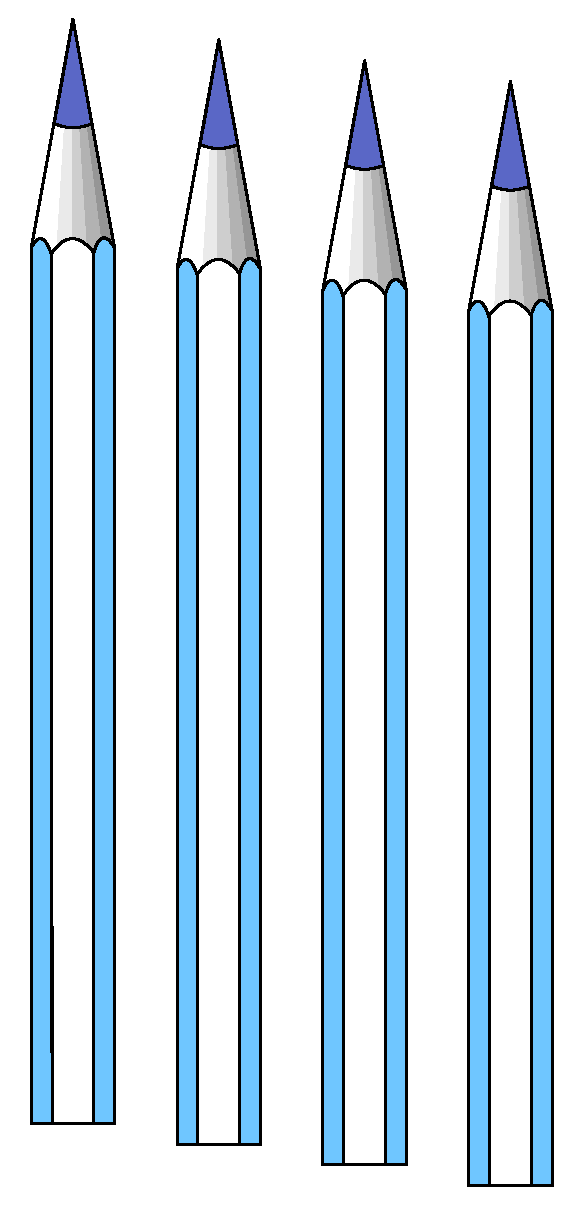
\includegraphics[angle=-90,width=0.9\textwidth]{pencils}}

  \vspace{\stretch{2}}

  {Wolfgang Dobler \& Axel Brandenburg}

  \vspace{\stretch{1}}

  \emph{$ $Date: 2003-07-15 07:05:32 $ $,~ $ $Revision: 1.182 $ $}

  \vspace{\stretch{3}}


\end{center}

\end{titlepage}


\newpage
\mbox{}
\vfill

Copyright \copyright{} 2001,2002 Wolfgang Dobler \& Axel Brandenburg
\bigskip

Permission is granted to make and distribute verbatim copies of
this manual provided the copyright notice and this permission notice
are preserved on all copies.

Permission is granted to copy and distribute modified versions
of this manual under the conditions for verbatim copying,
provided that the entire resulting derived work is distributed under the
terms of a permission notice identical to this one.


\clearpage
\pagestyle{plain}
\pagenumbering{roman}


% ====================================================================== %

\section*{Foreword}

This code was originally developed at the Turbulence Summer School of the
Helmholtz Institute in Potsdam (2001).
While some SPH and PPM codes for hydrodynamics and magnetohydrodynamics
are publicly available, this does not generally seem to be
the case for higher order finite-difference or spectral codes.
Having been approached by people interested in using our code, we
decided to make it as flexible as possible and as user-friendly as seems
reasonable, and to put it onto a public \name{CVS} repository.
The code can certainly not be treated as a black box (no code can), and in
order to solve a new problem in an optimal way, users will need to find their
own optimal set of parameters.
In particular, you need to be careful in choosing
the right values of viscosity, magnetic diffusivity, and radiative
conductivity.

The Pencil Code is primarily designed to deal with weakly compressible
turbulent flows, which is why we use high-order first and second derivatives.
To achieve good parallelization, we use explicit
(as opposed to compact) finite differences.
Typical scientific targets include driven MHD turbulence in a periodic box,
convection in a slab with non-periodic upper and lower boundaries,
a convective star embedded in a fully nonperiodic box, accretion disc
turbulence in the shearing sheet approximation, etc.

Magnetic fields are implemented in terms of the magnetic vector potential
to ensure that the field remains solenoidal (divergence-free).
At the same time, having the magnetic
vector potential readily available is a big advantage if
one wants to monitor the magnetic helicity, for example.
The code is therefore particularly well suited for all kinds of
dynamo problems.

The code is non-conservative; thus, conserved quantities should only be
conserved up to the discretization error of the scheme (not to machine
accuracy).
There is no guarantee that a conservative code is more accurate with
respect to quantities that are not explicitly conserved, such as entropy.
Another important quantity that is (to our knowledge) not strictly
conserved by ordinary flux conserving schemes is \name{magnetic helicity}.

There are currently no plans to implement adaptive mesh refinement
into the code, which would cause major technical complications.
Given that turbulence is generically space-filling, local refinement
to smaller scales would often not be very useful anyway.
On the other hand, in some geometries
turbulence may well be confined to certain regions in space, so one
could indeed gain by solving the outer regions with fewer points.

In order to be cache-efficient, we solve the equations along
\name{pencils} in the $x$ direction.
One very convenient side-effect is that auxiliary and derived variables
use very little memory, as they are only ever defined on one pencil.
The domain can be tiled in the $y$ and $z$ directions.
On multiprocessor computers, the code can use \name{MPI}
(Message Passing Interface) calls to communicate between processors.
An easy switching mechanism allows the user to run the code on a machine
without MPI libraries (e.g.~a notebook computer).
Ghost zones are used to implement boundary conditions on physical and
processor boundaries.

A high level of flexibility is achieved by encapsulating individual
physical processes and variables in individual \name{modules}, which can
be switched on or off in the file \file{Makefile.local} in the local
\file[src/]{src} directory.
This approach avoids the use of difficult-to-read preprocessor directives,
at the price of requiring one dummy module for each physics module.
For nonmagnetic hydrodynamics, for example, one will use the module
\file{nomagnetic.f90} and specifies
\begin{Verbatim}
  MAGNETIC=nomagnetic
\end{Verbatim}
in \file{Makefile.local},
while for MHD simulations, \file{magnetic.f90} will be used:
\begin{Verbatim}
  MAGNETIC=magnetic
\end{Verbatim}
Note that the term \name{module} as used here is only loosely related to
Fortran modules:
both \file{magnetic.f90} and \file{nomagnetic.f90} define an F90
module named \emph{Magnetic} --- this is the basis of the switching
mechanism we are using.

Input parameters (which are set in the files \file{start.in},
\file{run.in}) can be changed without recompilation.
Furthermore, one can change the list of variables for monitoring
(diagnostic) output on the fly, and there are mechanisms for making the
code reload new parameters or exit gracefully at runtime.

The requirements for using the Pencil-MPI code are modest: you can use it
on any Unix system with a F90/F95 compiler. If you have \name{IDL} as
well, you will be able to visualize the results (a number of sample
procedures are provided), but other tools such as
\name{DX} (OpenDX, data explorer) can also be used.

\bigskip

If you want to make creative use of the code, this manual will contain far
too little information.
Its major aim is to give you an idea of the way the code is organized, so
you can more efficiently \emph{read the source code}, which contains a
reasonable amount of comments.
You might want to read through the various run directories that are checked in.
Choose one that is closest to your application and start modifying.
For further enhancements that you may want to add to the code, you can
take as an example the lines in the code that deal with related variables,
functions, diagnostics, equations etc., which have already been implemented.
Just remember: \cmd{grep} is one of your best friends when you want to
understand how certain variables or functions are used in the code.

\bigskip

We will be happy to include user-supplied changes and updates to the code
in future releases and welcome any feedback.

\vspace{5mm}
%\noindent
\email{Wolfgang.Dobler@kis.uni-freiburg.de}\hfill Freiburg\\
\email{Axel.Brandenburg@nordita.dk}\hfill Copenhagen


% ====================================================================== %

\section*{Acknowledgments}

Many people have contributed in different ways to the development of this
code. We thank first of all {\AA}ke Nordlund (Copenhagen Observatory)
and Bob Stein (University of Michigan) who introduced us to the idea of
using high-order schemes in compressible flows and who taught us a lot
about simulations in general.

The calculation of the power spectra, structure functions, the remeshing procedures,
routines for changing the number of processors, as well as
the shearing sheet approximation and the flux-limited diffusion
approximation for radiative transfer
were implemented by Nils Erland L.\ Haugen (University of Trondheim).
Tobi Heinemann added the Feautrier method for radiative transfer as well as
hydrogen ionization.
Anders Johansen and Anja Andersen contributed to the implementation of
the dust equations.
Anthony (Tony) Mee (University of Newcastle) implemented shock viscosity
and Graeme R.\ Sarson (also University of Newcastle) added the
interstellar module.
Vladimir Pariev (University of Rochester) contributed to the development
and testing of the potential field boundary condition.

Use of the PPARC supported supercomputers in St Andrews (Mhd) and
Leicester (Ukaff) is acknowledged. We also acknowledge use of the
512 processor Beowulf cluster in Odense (Horseshoe).

\clearpage
\tableofcontents
\cleardoublepage
\pagestyle{fancy}
\pagenumbering{arabic}


% ====================================================================== %

\section{System Requirements}

To use the code, you will need the following:

\begin{enumerate}

  \item Absolutely needed:
    \begin{itemize}
    \item F90 or F95 compiler
    \end{itemize}

\item Used heavily (if you don't have one of these, you will need to
  adjust many things manually):
  \begin{itemize}
  \item a \name{Unix}-type system with \name{make} and \name{csh}
  \item \name{Perl} (remember: if it doesn't run Perl, it's not a
    computer)
  \end{itemize}

\item The following are dispensable, but enhance functionality in one
  way or the other:
  \begin{itemize}
  \item an \name{MPI} implementation (for parallelization on
    multiprocessor systems)
  \item a \name{C} compiler (for some debugging functionality)
  \item \name{DX} alias \name{OpenDX} or \name{data explorer} (for
    3-D visualization of results)
  \item \name{IDL} (for visualization of results; the 7-minute demo
    license will do for many applications)
  \end{itemize}

\end{enumerate}

%If you like the exotic and get the code running in a \name{Cygwin}
%environment, please let us know.


% ====================================================================== %

\section{Obtaining the Code}

There are two ways to obtain the code:
you can access the latest version via anonymous \name{CVS},
or you can download the tarball of a stable release.
Older tarballs are kept, and the correspondingly old version
of the manual is also checked in, but the manual on the web
refers of course to a recent version.

Since we are still actively developing the code (and probably always
will), it is important to be able to update your version to the current
one.
You can do so via \name{CVS}, regardless of whether you have initially
installed the tarball or have used \name{CVS} from the very start.

To ensure at least some level of stability of the \name{CVS}
versions, a set of test problems (listed in
\file[auto-test]{\$PENCIL_HOME/bin/auto-test})
are routinely tested.
This includes all problems in
\file[samples/]{\$PENCIL_HOME/samples}.

% ---------------------------------------------------------------------- %

\subsection{Obtaining the code via anonymous CVS}

\begin{enumerate}

\item Many machines have \name{CVS} installed
  (try \code{cvs -v} or \code{which cvs}).
  If yours have not, get a \name{CVS} client from
  \url{http://www.cvshome.org/} and
  install it on any machine where you want to run the code.
  Alternatively, just copy the executable from a binary compatible
  machine.

\item Get the password for anonymous \name{CVS} access to the Pencil Code
  from the download section in
  \path{http://www.nordita.dk/data/brandenb/pencil-code}.
  Alternatively, just email \email{Wolfgang.Dobler@kis.uni-freiburg.de}
  or \email{Axel.Brandenburg@nordita.dk}.
  Privileged users with write access to the original repository should
  continue to use it.\footnote{%
    In that case you'd say
    \code{setenv CVSROOT :pserver:\$USER@norserv.nordita.dk:/home/brandenb/CVS},
    assuming that \env[USER]{\$USER} is the userid registered in the original
    repository. The content of this repository is copied automatically every
    hour to the anonymous cvs repository.
    Be sure to run \code{auto-test} before you check anything back in again.
    It can be very annoying for someone else to figure out what's wrong,
    especially if you are just up to something else.}

\item Set your environment variable \env{CVSROOT}:
  \begin{small}
  \begin{alltt}
  \prompt{csh> } setenv CVSROOT :pserver:anonymous@norserv.nordita.dk:/home/cvs/public \
  \end{alltt}
  \end{small}
  or (if you are running \name{bash} or \name{Bourne shell})
  \begin{small}
  \begin{alltt}
  \prompt{sh> } CVSROOT=:pserver:anonymous@norserv.nordita.dk:/home/cvs/public
  \prompt{sh> } export CVSROOT \
  \end{alltt}
  \end{small}

\item Log in:
  \begin{alltt}
  \prompt{unix> } cvs login
  cvs password: ........ \
\end{alltt}
(you only need to do this once; your CVS password is saved in the file
\file{.cvspass} in your home directory)

\item Go to wherever you want the code:
  \begin{alltt}
  \prompt{unix> } cd somewhere/ \
  \end{alltt}
  and check out the code:
  \begin{alltt}
  \prompt{unix> } cvs checkout pencil-code \
  \end{alltt} 
  This creates a subdirectory \file[pencil-code/]{somewhere/pencil-code}
  and populates it with the Pencil Code's subdirectories.
  If you change your mind about the location of the code, you can just
  move the whole directory,
  \begin{alltt}
  \prompt{unix> } mv somewhere/pencil-code elsewhere/ \
  \end{alltt}
  since \name{CVS} keeps all information in the local \file{CVS/}
  subdirectories below \file{pencil-code/}.
\end{enumerate}


% ---------------------------------------------------------------------- %

\subsection{Obtaining and unpacking the tarball}

\begin{enumerate}
\item Download the tarball \texttt{pencil-code_\emph{X}.tar.gz}
  (where \emph{X} is the release number) from the download section in
  \url{http://www.nordita.dk/data/brandenb/pencil-code}

\item Put it into a convenient directory and unpack it:
  \begin{alltt}
  \prompt{unix> } mv pencil-code_\emph{X}.tar.gz somewhere/
  \prompt{unix> } cd somewhere
  \prompt{unix> } gunzip pencil-code_\emph{X}.tar.gz
  \prompt{unix> } tar xf pencil-code_\emph{X}.tar \
  \end{alltt}
\end{enumerate}

% ---------------------------------------------------------------------- %

\subsection{Updating via CVS}

Independent of how you installed the code in the first place (from tarball
or via \name{CVS}), you can update your version using \name{CVS}.
If you have done nontrivial alterations to your version of the code, you
ought to be careful about upgrading: although \name{CVS} is an excellent
tool for distributed programming,
conflicts are quite likely, since we are going to
touch many parts of the code while we develop it further.
Thus, despite the fact that the code is under \name{CVS}, you should probably
back up your changes before upgrading.

Here is the upgrading procedure:
\begin{enumerate}
\item Go to the top directory of the code:
  \begin{alltt}
  \prompt{unix> } cd somewhere/pencil-code \
  \end{alltt}
\item Run \cmd{cvs update}:
  \begin{alltt}
  \prompt{unix> } cvs -q update -dP \
  \end{alltt}
  (the option \option{-q} means ``somewhat quiet'', \option{-d} checks out
  new directories, and \option{-P} removes empty directories)
\item Fix any conflicts you encounter and make sure the examples in the
  directory \file{samples/} are still working.
\end{enumerate}

% ---------------------------------------------------------------------- %

\subsection{Getting older versions}

You may find that the latest \name{CVS} version of the code produces errors.
If you have reasons to believe that this is due to changes introduced on
27 November 2002 (to give an example), you can check out the version prior to
this by:
\begin{enumerate}
\item Go to the top directory of the code:
  \begin{alltt}
  \prompt{unix> } cd somewhere/pencil-code \
  \end{alltt}
\item Run \cmd{cvs update}:
  \begin{alltt}
  \prompt{unix> } cvs up -D "26 Nov 2002"\
  \end{alltt}
\end{enumerate}

% ---------------------------------------------------------------------- %

\subsection{Obtaining and unpacking the tarball}

\begin{enumerate}
\item Download the tarball file, pencil-code_X.tar.gz,
  where X is the release number, after registering on
  \path{http://www.nordita.dk/data/brandenb/pencil-code/}
\item Put it into a convenient directory and unpack it:
  \begin{alltt}
  \prompt{unix> } mv pencil-code_X.tar.gz somewhere/; cd somewhere
  \prompt{unix> } gunzip pencil-code_X.tar.gz
  \prompt{unix> } tar xf pencil-code_X.tar \
  \end{alltt}
\end{enumerate}


% ====================================================================== %

\section{Getting Started}
\label{S-getting-started}

To get yourself started, you should run one or several examples which are
provided in one of the \file{samples/} subdirectories.
Note that you will only be able to fully assess the numerical solutions if you
visualize them with \name{IDL}, \name{DX} or other tools (see
Sect.~\ref{S-Visualization}).

% ---------------------------------------------------------------------- %

\subsection{Setup}

\subsubsection{Environment settings}

The functionality of helper scripts and IDL routines relies on a few
environment variables being set correctly.
The simplest way to achieve this is to go to the top directory of the code
and source one of
the two scripts \file{sourceme.csh} or \file{sourceme.sh} (depending on
the type of shell you are using):
\begin{alltt}
  \prompt{csh> } cd pencil-code
  \prompt{csh> } source ./sourceme.csh
\end{alltt}
for \name{tcsh} or \name{csh} users; or
\begin{alltt}
  \prompt{sh> } cd pencil-code
  \prompt{sh> } . ./sourceme.sh
\end{alltt}
for users of \name{bash}, \name{Bourne shell}, or similar shells.
You should get output similar to
\begin{alltt}
  PENCIL_HOME = </home/dobler/f90/pencil-code>
  Adding /home/dobler/f90/pencil-code/bin to PATH
\end{alltt}
Apart from the \env{PATH} variable, the environment variable
\env{IDL_PATH} is set to something like
\texttt{./idl:../idl:+\$PENCIL_HOME/bin:./data:<IDL_DEFAULT>} .

\paragraph{Note 1}
The \code{<IDL_DEFAULT>} mechanism does not work for IDL versions 5.2 or
older. In this case, you will have to edit the path manually, or adapt
the \file{sourceme} scripts.

\paragraph{Note 2}
If you  don't want to rely on the \file{sourceme} scripts' (quite
heuristic) ability to correctly identify the code's main directory, you
can set the environment variable
\env{PENCIL_HOME} explicitly before you run the source command.

\paragraph{Note 3}
The second time you source \file{sourceme}, it will not add
anything to your \env{PATH} variable.
This is on purpose to avoid cluttering of your environment: you can
source the file as often as you like (in your shell startup script, then
manually and in addition in some script you have written), without
thinking twice.
If, however, at the first sourcing, the setting of \env{PENCIL_HOME} was
wrong, this mechanism would keep you from ever adding the right directory
to your \env{PATH}.
In this case, you need to first undefine the environment variable
\env{PENCIL_HOME}:
\begin{alltt}
  \prompt{csh> } unsetenv PENCIL_HOME
  \prompt{csh> } source ./sourceme.csh
  {\sl{}or}
  \prompt{sh> } unset PENCIL_HOME
  \prompt{sh> } . ./sourceme.sh
\end{alltt}



\subsubsection{Linking scripts and source files}

With your environment set up correctly, you can now go to the directory
you want to work in and set up subdirectories and links.
This is accomplished by the script \file{setup-src}, which is located in
\file[bin/]{\$PENCIL_HOME/bin} and is thus now in your executable path.

For concreteness, let us assume you want to use
\file[conv-slab/]{samples/conv-slab}
as your \dfn{run directory}, i.e.\ you want to run a three-layer slab model
of solar convection.
You then do the following:
\begin{alltt}
  \prompt{unix> } cd samples/conv-slab
  \prompt{unix> } setup-src
  src already exists
  2 files already exist in src
\end{alltt}
The script has linked a number of scripts from \file[bin/]{\$PENCIL_HOME/bin},
generated a directory \file[src/]{src} for the source code and linked the
Fortran source files (plus a few more files) from \file[src/]{\$PENCIL_HOME/src}
to that directory:
\begin{alltt}
  \prompt{unix> } ls -F
  CVS/           src/
  start.csh@     run.csh@  getconf.csh@ 
  start.in       run.in    print.in            
  reference.out     
\end{alltt}


\subsubsection{Adapting the Makefile}

This step requires some input from you, but you only have to do this once
for each machine you want to run the code on.
See Sect.~\ref{adapt-mkfile} for a description of the steps you need to
take here.
(If you are lucky and use compilers similar to the ones we have, you may
be able to skip this step; but blame yourself if things don't compile, then.)


\subsubsection{Running \cmd{make}}

Next, you run \cmd{make} in the \file[src/]{src} subdirectory of your run
directory.
Since you are using one of the predefined test problems, the settings in
\file[Makefile.local]{src/Makefile.local} and
\file[cparam.local]{src/cparam.local} are all reasonable, and you just do
\begin{alltt}
  \prompt{unix> } cd src
  \prompt{unix> } make \
\end{alltt}
If you have set up the compiler flags correctly, compilation should
complete successfully, and you can return to the run directory,
\begin{alltt}
  \prompt{unix> } cd .. \
\end{alltt}


\subsubsection{Choosing a data directory}

The code will by default write data like snapshot files to the subdirectory
\file[data/]{data} of the run directory.
Since this will involve a large volume of IO-operations (at least for
large grid sizes), one will normally try to avoid writing the data via
NFS.
The recommended way to set up a \file[data/]{data} data directory is to generate
a corresponding directory on the local disc of the computer you are
running on and (soft-)link it to \file[data/]{./data}.
Even if the link is part of an NFS directory, all the IO operations will
be local.
For example, if you have a local disc \file[/scratch/]{/scratch}, you can
do the following
\begin{alltt}
  \prompt{unix> } mkdir -p /scratch/\$USER/pencil-data/samples/conv-slab
  \prompt{unix> } ln -s /scratch/\$USER/pencil-data/samples/conv-slab ./data \
\end{alltt}

Even if you don't have an NFS-mounted directory (say, on your notebook
computer), it is probably still a good idea to have code and data well
separated by a scheme like the one described above.

An alternative to symbolic links, is to provide a file called 
\file{datadir.in} in the root of the run directory.  This file
should contain one line of text specifying the absolute or relative data 
directory path to use.  This facility is useful if one wishes to switch
one run directory between different data directories.  It is suggested
that in such cases symbolic links are again made in the run directory
to the various locations, then the \file{datadir.in} need
contain only a short relative path.


\subsubsection{Running the code}

You are now ready to start the code:
\begin{alltt}
  \prompt{unix> } start.csh\small
  Linux cincinnatus 2.4.10-4GB #1 Tue Sep 25 12:33:54 GMT 2001 i686 unknown
  Non-MPI version
  Thu Jul 18 16:25:20 CEST 2002
     src/start.x
  CVS: hydro.f90          v. 1.48         (dobler    ) 2002/07/19 10:26:01
  {\sl{}[\ldots]}
  CVS: start.in           v. 1.2          (dobler    ) 2002/07/19 10:23:57
   mx,my,mz=          38          38          38
   
   uu: up-down
   piecewise polytropic vertical stratification (lnrho)
   init_lnrho: cs2bot,cs2top=   1.450000      0.3333330    
   piecewise polytropic vertical stratification (ss)
   Note: mpoly{1,2} override hcond{1,2} to    2.000000      0.5000000    
   
  0.060u 0.000s 0:00.24 25.0\%     0+0k 0+0io 126pf+0w
  
  Fri Jul 19 13:04:38 CEST 2002
\end{alltt}
This runs \file[start.x]{src/start.x} to construct an initial condition based on
the parameters set in \file{start.in}.
This initial condition is stored in \file[var.dat]{data/proc0/var.dat} (and
in \file[var.dat]{data/proc1/var.dat}, etc.\ if you run the multiprocessor
version).

% ---------------------------------------------------------------------- %
\begin{figure}[hbtp]
  \centering
  \includegraphics%
    [width=1\textwidth,keepaspectratio]%
    {pvert0}
  \caption{Initial state of the three-layer convection model in
    \file[conv-slab/]{samples/conv-slab}.
    Shown are (from left to right) density $\varrho$, vertical velocity
    $u_z$, entropy $s/c_p$ and temperature $T$ as functions of the
    vertical coordinate $z$ for about ten different vertical lines in the
    computational box.
    The dashed lines denote domain boundaries:
    $z<-0.68$ is the lower ghost zone (points have no physical significance);
    $-0.68<z<0$ is a stably stratified layer ($ds/dz>0$);
    $0<z<1$ is the unstable layer ($ds/dz<0$);
    $1<z<1.32$ is the isothermal top layer;
    $z>1.32$ is the upper ghost zone (points have no physical significance).
  }
  \label{Fig-pvert0}
\end{figure}
% ---------------------------------------------------------------------- %

If you have IDL, you can visualize the initial state with (see
Sect.~\ref{S-IDL-routines} for details)
\begin{alltt}
  \prompt{unix > } idl
  \prompt{IDL >  } .r start
  \prompt{IDL >  } .r r
  \prompt{IDL >  } .r thermo
  \prompt{IDL >  } .r pvert \
\end{alltt}
The result should look like in Fig.~\ref{Fig-pvert0}.

\bigskip

Now we run the code:
\begin{alltt}
  \prompt{unix> } run.csh
\end{alltt}
This runs \file[run.x]{src/run.x} and carries out \var{nt} time steps, where
\var{nt} and other run time parameters are specified in \file{run.in}.
On a decent PC (1.7\,GHz), 1000 time steps take about 3 minutes.

The relevant part of the code's output looks like\\
\begin{minipage}{1\textwidth}
\bigskip
\begin{small}
\begin{alltt}
---it------t--------dt--------urms------umax------rhom------ssm-------dtc----
      0     0.00  8.561E-03   0.00633   0.09560   14.4708  -0.44601  4.74E-01
     50     0.43  8.555E-03   0.00498   0.04376   14.4706  -0.44563  4.74E-01
    100     0.86  8.548E-03   0.00428   0.03027   14.4706  -0.44523  4.74E-01
    150     1.28  8.551E-03   0.00380   0.02265   14.4707  -0.44491  4.74E-01
    200     1.71  8.554E-03   0.00352   0.01872   14.4710  -0.44528  4.74E-01
    250     2.14  8.551E-03   0.00310   0.01352   14.4716  -0.44515  4.74E-01
    300     2.57  8.555E-03   0.00284   0.01506   14.4715  -0.44489  4.74E-01
    350     2.99  8.555E-03   0.00257   0.01426   14.4713  -0.44461  4.74E-01
    400     3.42  8.557E-03   0.00253   0.01304   14.4712  -0.44484  4.74E-01
    450     3.85  8.557E-03   0.00261   0.01305   14.4713  -0.44504  4.74E-01
    500     4.28  8.557E-03   0.00269   0.01375   14.4716  -0.44567  4.74E-01
    550     4.71  8.559E-03   0.00266   0.01490   14.4716  -0.44604  4.74E-01
    600     5.13  8.559E-03   0.00308   0.01481   14.4713  -0.44584  4.74E-01
    650     5.56  8.560E-03   0.00333   0.01543   14.4712  -0.44555  4.74E-01
    700     5.99  8.559E-03   0.00361   0.01604   14.4713  -0.44541  4.74E-01
    750     6.42  8.559E-03   0.00402   0.01723   14.4715  -0.44562  4.74E-01
    800     6.85  8.558E-03   0.00449   0.02000   14.4718  -0.44565  4.74E-01
    850     7.27  8.558E-03   0.00507   0.02277   14.4716  -0.44542  4.74E-01
    900     7.70  8.559E-03   0.00575   0.02599   14.4713  -0.44527  4.74E-01
    950     8.13  8.560E-03   0.00658   0.02860   14.4712  -0.44543  4.74E-01
\end{alltt}
\end{small}
\bigskip
\end{minipage}
and lists
\begin{enumerate}
\item the number \var{it} of the current time step; 
\item the time, \var{t};
\item the time step, \var{dt};
\item the rms velocity, \var{urms}$=\sqrt{\left<\uv^2\right>}$;
\item the maximum velocity, \var{umax}$=\max |\uv|$;
\item the mean density, \var{rhom}$=\left<\varrho\right>$;
\item the mean entropy, \var{ssm}$=\left<s\right>/c_p$;
\item the time step in units of the acoustic Courant step,
  \var{dtc}$=\delta t/({\cs}_0\,\delta x_{\rm min})$.
\end{enumerate}
The entries in this list can be added, removed or reformatted in the file
\file{print.in}, see Sects~\ref{diagnostic-IO} and \ref{S-print.in-run-params}.

To visualize the resulting state, run
\begin{alltt}
  \prompt{IDL >  } .r r
  \prompt{IDL >  } .r pvert \
\end{alltt}
and you should obtain something similar to Fig.~\ref{Fig-pvert1}, which
corresponds to the state after 1000 time steps.

% ---------------------------------------------------------------------- %
\begin{figure}[hbtp]
  \centering
  \includegraphics%
    [width=1\textwidth,keepaspectratio]%
    {pvert1}
  \caption{Like in Fig.~\ref{Fig-pvert0}, but after 1000 time steps at
    time $t=7.0$.
    The dashed lines represents the initial condition.
  }
  \label{Fig-pvert1}
\end{figure}
% ---------------------------------------------------------------------- %

For the evolution of velocity and the state at later times, see
Sect.~\ref{S-ref-data} in the Appendix.


\paragraph{Note:}
If you want to run the code with \name{MPI}, you will probably need to
adapt \file{getconf.csh}, which defines the commands and flags used to
run MPI jobs (and which is sourced by the scripts \file{start.csh} and
\file{run.csh}).
Try
\begin{alltt}
  csh -v getconf.csh
  {\sl or}
  csh -x getconf.csh
\end{alltt}
to see how \file{getconf.csh} makes its decisions. You would add a
section for the host name of your machine with the particular settings.
Since \file{getconf.csh} is linked from the central directory
\file[bin/]{pencil-code/bin}, your changes will be
useful for all your other runs too.

% ---------------------------------------------------------------------- %

\subsection{A second test}

We will add other simple examples (periodic, isothermal, non-forced MHD)
where the physics is already nontrivial.
The following is not available yet.

\subsubsection{Interlocked flux rings}

\begin{alltt}
  \prompt{unix> } cd somewhere/pencil-code
  \prompt{unix> } source sourceme.csh \quad\#(to put pencil-code/bin into your path)
  \prompt{unix> } cd runs/sample/rings
  \prompt{unix> } setup-src \quad\#(from \file[bin/]{../../../bin}, which by now should be in your path)
  \prompt{unix> } cd src
  \prompt{unix> } make
  \prompt{unix> } cd ..
  \prompt{unix> } mkdir data \quad{\sl\# (or [better] link directory on local disc to \file[data/]{data})}
  \prompt{unix> } ./start.csh
  \prompt{unix> } ./run.csh
\end{alltt}

The output should look like \ldots

% ---------------------------------------------------------------------- %

\subsection{Other test problems}

\begin{alltt}
   conv-slab  conv-slab-flat  helical-MHDturb  interlocked-fluxrings
\end{alltt}


% ====================================================================== %

\section{Code structure}

\subsection{Directory tree}

 % ---------------------------------------------------------------------- %
\begin{figure}[hbtp]
  \centering
  \includegraphics%
    [width=0.9\textwidth,height=0.65\textheight,keepaspectratio]%
    {struct}
  \caption{The basic structure of the code}
  \label{Fig-Structure}
\end{figure}
% ---------------------------------------------------------------------- %

The overall directory structure of the code is shown in
Fig.~\ref{Fig-Structure}.
Under \file[pencil-code/]{pencil-code}, there are currently the following
files and directories:
\begin{verbatim}
  CVS/      bin/    bugs/           doc/
  dx/       idl/    samples/        src/
  README    TODO    sourceme.csh    sourceme.sh
\end{verbatim}

Almost all of the source code is contained in the directory \file{src/},
but in order to encapsulate individual applications, the code is compiled
separately for each run in a local directory \file[src/]{src} below the
individual run directory, like
e.\,g.~\file[conv-slab/src/]{samples/conv-slab/src}.

It may be a good idea to keep your own runs also under \name{CVS}, but
this would normally be a different repository. On the machine where you
are running the code, you may want to check them out into a subdirectory
of \file{pencil-code/}.
For example, we have our own runs in a repository called
\file[pencil-runs/]{pencil-runs}, so we do
\begin{alltt}
  \prompt{unix> } cd \$PENCIL_HOME
  \prompt{unix> } cvs co -d runs pencil-runs
\end{alltt}
In this case, \file[runs/]{runs} contains individual run directories,
grouped in
classes (like \file[spher/]{spher} for spherical calculations, or
\file[kinematic/]{kinematic} for kinematic dynamo simulations).
The current list of classes in our own \file{pencil-runs} repository is
\begin{verbatim}
  1d-tests/   disc/          kinematic/  rings/
  2d-tests/   discont/       Misc/       slab_conv/ 
  3d-tests/   discussion/    OLD/        test/
  buoy_tube/  forced/        pass_only/
  convstar/   interstellar/  radiation/
\end{verbatim}
The directory \file{forced/} contains some forced turbulence runs (both
magnetic and nonmagnetic);
\file{gravz/} contains runs with vertical gravity;
\file{rings/} contains decaying MHD problems (interlocked flux rings as
initial condition, for example);
and \file{kinematic/} contains kinematic dynamo problems where the
hydrodynamics is turned off entirely.
The file \file{samples/README} should contain an up-to-date list and
short description of the individual classes.\footnote{Our
\file[pencil-runs/]{pencil-runs} directory also contains runs that were
done some time ago. Occasionally, we try to update these, especially if we
have changed names or other input convections.}

The subdirectory \file[src/]{src} of each run directory contains a few local
configuration files (currently these are \file{Makefile.local} and
\file{cparam.local}). To compile the sample links to
all the \file[*.f90]{.f90} and \file[*.c]{.c} files and the \file{Makefile} in the top
\file[src/]{src} directory must be created.  These links are set up by the script
\cmd{setup-src}) when used in a the root of run directory.

General-purpose visualization routines for \name{IDL} or \name{DX} are in the
directories \file[idl/]{idl} and \file[dx/]{dx}, respectively.
There are additional and more specialized \name{IDL} directories in the
different branches under \file[pencil-runs/]{pencil-runs}.

The directory \file[doc/]{doc} contains this manual;
\file[bin/]{bin} contains a number of utility scripts (mostly written in
\name{csh} and \name{Perl}), and in particular the \file{start.csh},
\file{run.csh}, and \file{getconf.csh} scripts.
The \file[CVS/]{CVS} directory is used (you guessed it) by \name{CVS}, and is
not normally directly accessed by the user;
\file[bugs/]{bugs}, finally is used by us for internal purposes.

\bigskip

The files \file{sourceme.csh} and \file{sourceme.sh} will set up some
environment variables --- in particular \env{PATH} --- and aliases/shell
functions for your convenience.
If you do not want to source one of these files, you need to make sure
your \name{IDL} path is set appropriately (provided you want to use
\name{IDL}) and you will need to address the scripts from
\file[bin/]{bin} with their explicit path name, or adjust your \env{PATH}
manually.



% ---------------------------------------------------------------------- %

\subsection{Basic concepts}

\subsubsection{Data access in pencils}
\index{Pencil design}

Unlike the CRAY computers that dominated supercomputing in the 80s and
early 90s, all modern computers have a cache that constitutes a significant
bottleneck for many codes.
This is the case if large three-dimensional arrays are constantly used
within each time step, which has the obvious advantage of working on
long arrays and allows vectorization of elementary machine operations.
This approach also implies
conceptual simplicity of the code and allows extensive use of the
intuitive F90 array syntax.
However, a more  cache-efficient way of coding is to calculate an entire
time step
(or substep of a multi-stage time-stepping scheme) only
along a one-dimensional pencil of data within the numerical grid.
This technique is more efficient for modern RISC processors:
on Linux PCs and SGI workstations, for example, we have found a speed-up
by about 60\%{} in some cases.
An additional advantage is a drastic reduction in temporary storage for
auxiliary variables within each time step.

\subsubsection{Modularity}
\label{S-modularity}
\index{Modules}

Each run directory has a file \file[Makefile.local]{src/Makefile.local} in
which you
choose certain \name{modules}\footnote{%
  We stress once more that we are not talking about F90 modules here,
  although there is some connection, as most of our modules define F90
  modules:
  For example each of the three modules \name{grav_z}, \name{grav_r} and
  \name{nograv} defines a Fortran module \name{Gravity}.
}, which tell the code whether or not entropy, magnetic fields,
hydrodynamics, forcing, etc.\ should be invoked.
For example, the settings for forced turbulent MHD simulations are
\begin{verbatim}
  HYDRO     =   hydro
  DENSITY   =   density
  ENTROPY   = noentropy
  MAGNETIC  =   magnetic
  GRAVITY   = nograv
  FORCING   =   forcing
    
  MPICOMM   = nompicomm
  GLOBAL    = noglobal
  IO        =   io_dist
  FFT       = nofft
\end{verbatim}
This file will be processed by \name{make} and the settings are thus
assignments of \name{make} variables.
Apart from the physics modules (equation of motion: yes, density
[pressure]: yes, entropy equation: no, magnetic fields: yes, gravity: no,
forcing: yes), a few technical modules can also be used or deactivated; in
the example above, these are \name{MPI} (switched off), additional global
variables (none), input/output (distributed), and \name{FFT} (not used).
Table~\ref{Tab-modules} in the Appendix lists all currently available modules.

Note that most of these \name{make} variables \emph{must} be set, but they
will normally obtain reasonable default values in \file{Makefile} (so you
only need to set the non-standard ones in \file{Makefile.local}).
It is by using this switching mechanism through \cmd{make} that we achieve
high flexibility without resorting to excessive amounts of cryptic
preprocessor directives or other switches within the code.
 
Many possible combinations of modules have already been tested
and examples are part of the distribution, but you may be interested in a
combination which was never tried before and which may not work yet, since the
modules are not fully orthogonal.
In such cases, we depend on user feedback for fixing problems
and documenting the changes for others.


% ---------------------------------------------------------------------- %

\subsection{Files in the run directories}

\subsubsection{\file{start.in}, \file{run.in}, \file{print.in}}
These files specify the startup and runtime parameters (see
Sects.~\ref{S-start-params} and \ref{S-all-run-params}), and the list of
diagnostic variables to print (see \ref{diagnostic-IO}).
They specify the setup of a given simulation and are kept under CVS in
the individual \file[samples/]{samples} directories.

\subsubsection{\file{datadir.in}}
\label{Ss-datadir-in}
If this file exists, it must contain the name of an existing directory,
which will be used as \dfn{data directory},
i.\,e.~the directory where all results are written.
If \file{datadir.in} does not exist, the data directory is \file{data/}.

\subsubsection{\file{reference.out}}
If present, \file{reference.out} contains the output you should obtain in
the given run directory, provided you have not changed any parameters.
To see whether the results of your run are OK, compare \file{time_series.dat} to
\file{reference.out}:
\begin{alltt}
  \prompt{unix> } diff data/time_series.dat reference.out
\end{alltt}

\subsubsection{\file{start.csh}, \file{run.csh}, \file{getconf.csh}}
\label{start-run-getconf}
These are links to \file[bin/]{\$PENCIL_HOME/bin}.
You will be constantly using the scripts \file{start.csh} and
\file{run.csh} to initialize the code.
Things that are needed by both (like the name of the \cmd{mpirun}
executable, \name{MPI} options, or the number of processors) are located in
\file{getconf.csh}, which is never directly invoked.

\subsubsection{\file{src/}}
The \file[src/]{src} directory contains two local files,
\file[Makefile.local]{src/Makefile.local} and
\file[cparam.local]{src/cparam.local}, which allow the user to choose
individual modules (see \ref{S-modularity}) and to set parameters like the
grid size and the number of processors for each direction.
These two files are part of the setup of a given simulation and are kept
under CVS in the individual \file[samples/]{samples} directories.

The file \file[cparam.inc]{src/cparam.inc} is automatically generated by
the script \file{mkcparam} and contains the number of fundamental
variables for a given setup.

All other files in \file{src/} are either links to source files (and the
Makefile) in the \file[src/]{\$PENCIL_HOME/src} directory, or object and
module files generated by the compiler.

\subsubsection{\file{data/}}
This directory (the name of which will actually be overwritten by the first
line of \file{datadir.in}, if that file is present; see
\S\ref{Ss-datadir-in})
contains the output from the code:

\paragraph{\file[dim.dat]{data/dim.dat}}
The global array dimensions.

\paragraph{\file[legend.dat]{data/legend.dat}}
The header line specifying the names of the diagnostic variables in
\file{time_series.dat}.

\paragraph{\file[time_series.dat]{data/time_series.dat}}
Time series of diagnostic variables (also printed to stdout).
You can use this file directly for plotting with \name{Gnuplot},
\name{IDL}, \name{Xmgrace} or similar tools (see also
\S\ref{S-Visualization}).

\paragraph{\file[tsnap.dat]{data/tsnap.dat}, \file[tvid.dat]{data/tvid.dat}}
Time when the next snapshot \file{VAR$N$} or animation slice should be
taken.

\paragraph{\file[params.log]{data/params.log}}
Keeps a log of all your parameters: \file{start.x} writes the startup
parameters to this file, \file{run.x} appends the runtime parameters and
appends them anew, each time you use the \file{RELOAD} mechanism (see
\S\ref{S-RELOAD}).

\paragraph{\file[param.nml]{data/param.nml}}
Complete set of startup parameters, printed as Fortran namelist.
This file is read in by \file{run.x} (this is how values of startup
parameters are propagated to \file{run.x}) and by \name{IDL} (if you use
it).

\paragraph{\file[param2.nml]{data/param2.nml}}
Complete set of runtime parameters, printed as Fortran namelist.
This file is read by \name{IDL} (if you use it).

\paragraph{\file[index.pro]{data/index.pro}}
Can be used as include file in \name{IDL} and contains the column in which
certain variables appear in the diagnostics file (\file{time_series.dat}).
It also contains the positions of variables in the \file{VAR$N$} files.
These positions depend on whether \name{entropy} or \name{noentropy}, etc,
are invoked.
This is a temporary solution and the file may disappear in future
releases.

\paragraph{\file[interstellar.dat]{data/interstellar.dat}} 
Unformatted file containing the time at which the next supernova event will 
occur, under certain supernova schemes.  
(Only needed by the \name{interstellar} module.)

\paragraph{\file[proc$N$]{data/proc0}, \file[proc1]{data/proc1}, \ldots}
These are the directories containing data from the individual processors.
So after running an \name{MPI} job on two processors, you will have the
two directories \file[proc0]{data/proc0} and \file[proc1]{data/proc1}.
Each of the directories can contain the following files:
\begin{description}
\item[\file{var.dat}] binary file containing the latest snapshot;
\item[\file{VAR$N$}] binary file containing individual snapshot number $N$;
\item[\file{dim.dat}] ASCII file containing the array dimensions as seen
  by the given processor;
\item[\file{time.dat}] ASCII file containing the time corresponding to
  \file{var.dat};
\item[\file{grid.dat}] binary file containing the part of the grid seen by
  the given processor;
\item[\file{seed.dat}] the random seed for the next time step (saved for
  reasons of reproducibility).
  For multi-processor runs with velocity forcing, the files
  \file[seed.dat]{proc$N$/seed.dat} must all contain the same numbers,
  because globally coherent waves of given wavenumber are used;
\item[{\file[X.xy]{$X$.xy}, \file[X.xz]{$X$.xz}, \file[X.yz]{$X$.yz}}]
  two-dimensional sections of variable $X$, where $X$ stands for the
  corresponding variable. The current list includes
\begin{verbatim}
  bx.xy  bx.xz  by.xy  by.xz  bz.xy  bz.xz  divu.xy  lnrho.xz
  ss.xz  ux.xy  ux.xz  uz.xy  uz.xz
\end{verbatim}
  Each processor writes its own slice, so these need to
  be reassembled if one wants to plot a full slice.
\end{description}


% ====================================================================== %

\section{Using the Code}
\label{Input-params}

\subsection{Adapting the Makefile}
\label{adapt-mkfile}

By default, one \file{makefile} will only work on a given class of
computers with identical (or at least similar) compilers.
One aim when building the Pencil Code was however to allow running the
code on different machines without needing to modify any file.
This, together with \name{CVS} allows you for example to very quickly
compare results for identical runs on different machines.

Our mechanism for picking the right set of compiler flags is based on the
\name{Perl} script \file{adapt-mkfile} in \file[bin/]{\$PENCIL_HOME/bin}, which
processes the file \file{Makefile} to a (localized) \file{makefile}
(if both \file{Makefile} and \file{makefile} are present, \cmd{make} will
use the latter).
You can view the full documentation for \file{adapt-mkfile} with the
command
\begin{alltt}
  \prompt{unix > } perldoc adapt-mkfile
\end{alltt}
provided \file[bin/]{\$PENCIL_HOME/bin} is in your path.

To give you an idea of how to add your own machines, let us assume you have
several Linux boxes running a compiler \cmd{f95} that needs the options
\option{-O4 -u}, while one of them, \name{Janus}, runs a compiler \cmd{f90}
which needs the flags \option{-O3} and requires the additional
options \option[-lmpi]{-lmpi -llam} for \name{MPI}.

The \file{Makefile} you need will have the following section:
\begin{alltt}
  ### Begin machine dependent
  
  ## IRIX64:
  {\sl{}[\ldots]   (leave as it is in the original Makefile)}
  ## OSF1:
  {\sl{}[\ldots]   (leave as it is in the original Makefile)}
  
  ## Linux:
  {\sl{}[\ldots]   (leave everything from original Makefile and add:)}
  #FC=f95
  #FFLAGS=-O4 -u
  #FC=f90             #(Janus)
  #FFLAGS=-O3         #(Janus)
  #LDMPI=-lmpi -llam  #(Janus)
  
  ## SunOS:
  {\sl{}[\ldots]   (leave as it is in the original Makefile)}
  ## UNICOS/mk:
  {\sl{}[\ldots]   (leave as it is in the original Makefile)}
  ## HI-UX/MPP:
  {\sl{}[\ldots]   (leave as it is in the original Makefile)}
  ## AIX:
  {\sl{}[\ldots]   (leave as it is in the original Makefile)}
  
  ### End machine dependent
\end{alltt}


\paragraph{Note 1}
If you have troubles with \cmd{make} or \file{adapt-mkfile}, look at the
\file{makefile} written by \file{adapt-mkfile} and check that it has the
entries for your machine activated.

\paragraph{Note 2}
If you want to experiment with compiler flags, --- or even if you just
want to get things running without setting up the machine-dependent
section of the makefile --- you can set \name{make} variables at the
command line.
E.\,g.
\begin{alltt}
  \prompt{src> } make FC=f90 FFLAGS='-fast -u'
\end{alltt}
will use the compiler \cmd{f90} and the flags
\option[-fast]{-fast -u} for both compilation and linking.


% ---------------------------------------------------------------------- %
\subsection{Changing the resolution}

It is advisable to produce a new run directory each time you run a new case.
(This does not include restarts from an old run, of course.)
If you have a $32^3$ run in some directory \file{runA_32a}, then go to
its parent directory, i.e.\
\begin{alltt}
  \prompt{runA_32a> } cd ..
  \prompt{forced> } new runA_32a runA_64a
  \prompt{forced> } cd runA_64a/src
  \prompt{forced> } vi cparam.local
\end{alltt}
and edit the \file{cparam.local} for the new resolution.

% ---------------------------------------------------------------------- %

\subsection{Diagnostic output}
\label{diagnostic-IO}

Every \var{it1} time steps (\var{it1} is a runtime parameter, see
Sect.~\ref{S-all-run-params}), the code writes monitoring output to
\name{stdout}
and, parallel to this, to the file \file[time_series.dat]{data/time_series.dat}.
The variables that appear in this listing and the output format are
defined in the file \file{print.in} and can be changed without touching
the code (even while the code is running).
A simple example of \file{print.in} may look like this:
\begin{verbatim}
  t(f10.3)
  urms(1pe13.4)
  rhom(0pf10.5)
  oum
\end{verbatim}
which means that the output table will contain time \var{t} in the first
column formatted as \verb|(f10.3)|, followed by the mean squared velocity,
\var{urms} (i.e.~$\left<\uv^2\right>^{1/2}$) in the second column with format
\verb|(1pe13.4)|, the average density \var{rhom} ($\left<\varrho\right>$,
which allows to monitor mass conservation) formatted \verb|(f10.5)| and
the kinetic helicity \var{oum}
(that is $\left<\vekt{\omega}\cdot\uv\right>$) in the last column with the
default format \verb|(1pe10.2)|.\footnote{
  Note that immediately after a format that uses the modifier \code{1p},
  one should switch back to \code{0p}, since otherwise the following numbers
  printed with \code{f} formats will be one order of magnitude off.
  This is the sad heritage of some more obscure Fortran I/O features.
}
The corresponding diagnostic output will look like
\begin{verbatim}
 ----t---------urms--------rhom------oum----
     0.000   4.9643E-03  14.42457 -8.62E-06
     0.032   3.9423E-03  14.42446 -5.25E-06
     0.063   6.8399E-03  14.42449 -3.50E-06
     0.095   1.1437E-02  14.42455 -2.58E-06
     0.126   1.6980E-02  14.42457 -1.93E-06
\end{verbatim}

In the file \file{zaver.in}, $z$-dependent (horizontal) averages are listed.
They are written to the file \file[zaverages.dat]{data/zaverages.dat}.
At the moment we
can also output in \file{print.in} the associated mean square value
of the horizontal field, but this requires that in \file{zaver.in} the
quantities \code{bxmz} and \code{bymz} are set.

% ---------------------------------------------------------------------- %

\subsection{Data files}
\index{datafiles}

\subsubsection{Snapshot files}
\label{snapshots}

Snapshot files contain the values of all evolving variables and are
sufficient to restart a run.
In the case of an MHD simulation with entropy equation, for example, the
snapshot files will contain the values of velocity, logarithmic density,
entropy and the magnetic vector potential.

There are two kinds of snapshot files: the current snapshot and permanent
snapshots, both of which reside in the directory
\file[data/proc$N$/]{data/proc$N$/}.
The parameter \var{isav} determines the frequency at which the
\emph{current snapshot} \file[var.dat]{data/proc$N$/var.dat} is written.
If you keep this frequency too high, the code will spend a lot of time on
I/O, in particular for large jobs; too low a frequency makes it
difficult to follow the evolution interactively during test runs.

The \emph{permanent snapshots} \file[VAR$N$]{data/proc*/VAR$N$} are
written every \var{dsnap} time units.
These files are numbered consecutively from $N=1$ upward and for long
runs they can occupy quite some disk space.
On the other hand, if after a run you realize that some additional
quantity $q$ would have been important to print out, these files are the
only way to reconstruct the time evolution of $q$ without re-running the
code.

Together with the raw data, the snapshot files contain the current
time $t$ and some other header information.
The script \cmd{tsnap} allows you to determine the time $t$ of a snapshot
file:
\begin{alltt}
  \prompt{unix> } tsnap data/proc0/var.dat
  data/proc0/var.dat:        t = 8.32456
  \prompt{unix> } tsnap data/proc0/VAR2
  data/proc0/VAR2:           t = 2.00603     
\end{alltt}


% \subsubsection{Averages}
% 
% [To be written]


% ---------------------------------------------------------------------- %

\subsection{Helper scripts}
\index{Scripts}

The \file[bin/]{bin} directory contains a collection of utility scripts,
some of which are discussed elsewhere,
Here is a list of the more important ones.

\begin{description}
\item[adapt-mkfile] Activate the settings in a \file{Makefile} that apply
  to the given computer, see \S\ref{adapt-mkfile}.
\item[auto-test] Verify that the code compiles and runs in a set of run
  directories and compare the results to the reference output.
  These tests are carried out routinely to ensure that the \name{CVS}
  version of the code is in a usable state.
\item[cleanf95] Can be use to clean up the output from the Intel x86 Fortran
  95 compiler (ifc).
\item[copy-proc-to-proc] Used for restarting in a different directory.
  Example \cmd{copy-proc-to-proc seed.dat ../hydro256e}.
\item[copy-snapshots] Copy snapshots from a processor-local directory to
  the global directory.
  To be started in the background before \file{run.x} is invoked.
  Used by \file{start.csh} and \file{run.csh} on network connected processors.
\item[copy-var-to-var] Copies all \file{var.dat} files from current directory
  to file{var.dat} in another run directory.
  Used for restarting in a different directory.
\item[copy-VAR-to-var] Used to restart a run from a particular snapshot 
  \file{VAR$N$}. Copies a specified snapshot \file{VAR$N$} to \file{var.dat}
  where $N$ and the target run directory are given on the command line.
\item[cvs-add-rundir] Add the current run directory to the CVS repository.
\item[cvsci_run] Similar to \cmd{cvs-add-rundir}, but it also checks in
  the \file{*.in} and \file{src/*.local} files. It also checks in the files
  \file[time_series.dat]{data/time_series.dat}, \file[dim.dat]{data/dim.dat} and
  \file[index.pro]{data/index.pro} for subsequent processing in
  \name{IDL} on another machine.
  This is particularly useful if collaborators want to check each others' runs.
\item[dx_*] These script perform several data collection or reformatting 
  exercises required to read particular files into \name{DX}.  They are
  called internally by some of the \name{DX} macros in the 
  \file[dx/macros/]{dx/macros/} directory.
\item[getconf.csh] See \S~\ref{start-run-getconf}
\item[gpgrowth] Plot simple time evolution with Gnuplot's ASCII graphics
  for fast orientation via a slow modem line.
\item[local] Materialize a symbolic link
\item[mkcparam] Based on \file{Makefile} and \file{Makefile.local},
  generate \file[cparam.inc]{src/cparam.inc}, which specifies the number
  \var{mvar} of fundamental variables, and \var{maux} of auxiliary 
  variables. Called by the \file{Makefile}.
\item[mkdatadir] Creates a link to a data directory in a suitable workspace.
  By default this is on \samp{/var/tmp/}, but different locations
  are specified for different machines.
\item[mkdotin] Generate minimal \file{start.in}, \file{run.in} files
  based on \file{Makefile} and \file{Makefile.local}.
\item[mkinpars] Wrapper around \samp{mkdotin} --- needs proper
  documentation.
\item[mkproc-tree] Generates a multi-processor(\file{proc$N$}/), directory 
  structure. Useful when copying data files in a processor tree, 
  such as slice files.
\item[mkwww] Generates a template HTML file for describing a run of the code,
  showing input parameters and results.
\item[move-slice] Moves all the slice files from a processor tree structure,
  \file[proc$N$]{proc$N$/}, to a new target tree creating directories where
  necessary.
\item[new] Generates a new run directory from an old one. The new one contains
  a copy of the old \file{*.local} files, runs \cmd{setup-src}, and
  makes also a copy of the old \file{*.in} and \file{k.dat} files.
\item[nl2idl] Transform a Fortran \name{namelist} (normally the files
  \file{param.nml}, \file{param2.nml} written by the code) into an
  \name{IDL} structure.
  Generates an \name{IDL} file that can be sourced from \file{start.pro}
  or \file{run.pro}.
\item[pacx-adapt-makefile] Version of adapt-makefile for highly 
  distributed runs using PACX MPI.
\item[read_videofiles.csh] The script for running read_videofiles.x.
\item[remote-top] Create a file \file{top.log} in the relevant 
  \file[proc$N$]{proc$N$/} directory containing the output of \code{top}
  for the appropriate processor. Used in batch scripts for 
  multi-processor runs.
\item[run.csh] The script for producing restart files with the initial
  condition; see \S~\ref{start-run-getconf}
\item[scpdatadir] Make a tarball of data directory, \file[data/]{data/} and 
  use \code{scp} to secure copy to copy it to the specified destination.
\item[setup-src] Link \file{start.csh}, \file{run.csh} and
  \file{getconf.csh} from \file[bin/]{\$PENCIL_HOME/bin}.
  Generate \file{src/} if necessary and link the source code files from
  \file[src/]{\$PENCIL_HOME/src} to that directory.
\item[start.csh] The script for initializing the code; see
  \S~\ref{start-run-getconf}
\item[summarize-history] Evaluate \file{params.log} and print a history 
  of changes.
\item[tst.csh] Execute \code{start.csh} and \code{run.csh} placing any output
  into a file called \code{.TEST.{`\it timestr}`}.
\item[timestr] Generate a unique time string that can be appended to file
  names from shell scripts through the backtick mechanism.
\item[tsnap] Extract time information from a snapshot file, \file{VAR$N$}.
\item[x] Check the execution of the current run: prints legend and the last
 few lines of the \file{time_series.dat} file. It also appends this result to a file
 called \file{SPEED}, which contains also the current wall clock time, so
 you can work out the speed of the code (without being affected by i/o time).
\end{description}

\vspace{5cm}

% ---------------------------------------------------------------------- %

\subsection{RELOAD and STOP files}
\label{S-RELOAD}

The code periodically (every \var{it} time steps) checks 
for the existence of two files, \file{RELOAD}
and \file{STOP}, which can be used to trigger certain behavior.


\paragraph{Reloading run parameters}
In the directory where you started the code, create the file
\file{RELOAD} with
\begin{alltt}
  \prompt{unix> } touch RELOAD \
\end{alltt}
to force the code to re-read the runtime parameters from \file{run.in}.
This will happen the next time the code is writing monitoring output (the
frequency of this happening is controlled by the input parameter \var{it},
see Sect.~\ref{S-start-params}).

[Occasionally, however, and only on some
machines, one of the processors may not survive the MPI barrier and
stops; we will need to look further into this.]

Each time the parameters are reloaded, the new set of parameters is
appended (in the form of \name{namelists}) to the file
\file[params.log]{data/params.log} together with the time $t$, so you have
a full record of your changes.
If \file{RELOAD} contains any text, its first line will be written to
\file[params.log]{data/params.log} as well, which allows you to annotate
changes:
\begin{alltt}
  \prompt{unix> } echo "Reduced eta to get fields growing" > RELOAD \
\end{alltt}


\paragraph{Stopping the code}
In the directory where you started the code, create the file
\file{STOP} with
\begin{alltt}
  \prompt{unix> } touch STOP \
\end{alltt}
to stop the code in a controlled manner (it will write the latest
snapshot).
Again, the action will happen the next time the code is writing monitoring
output.
% The \file{run.csh} removes any \file{STOP} files before starting
% \file{src/run.x}. If you run without the \file{run.csh} script you need
% to remember doing this by hand.

% ---------------------------------------------------------------------- %


\subsection{Start and run parameters}
\label{S-start-params}

All input parameters in \file{start.in} and \file{run.in}are grouped in
Fortran \name{namelists}.
This allows arbitrary order of the parameters (\emph{within} the given
namelist; the namelists need to appear in the correct order), as well as
enhanced readability through 
inserted Fortran comments and whitespace.
One namelist (\name{init_pars} / \name{run_pars}) contains general
parameters for initialization/running and is always read in.
All other namelists are specific to individual modules and will only
be read if the corresponding module is used.

The syntax of a namelist (in an input file like \file{start.in}) is
\begin{verbatim}
  &init_pars
    ip=5, Lxyz=2,4,2
  /
\end{verbatim}
--- in this example, the name of the namelist is \name{init_pars}, and we
read just two variables (all other variables in
the namelist retain their previous value): \var{ip}, which is set to $5$,
and \var{Lxyz}, which is a vector of length three and is set to $(2,4,5)$.

While all parameters from the namelists can be set, in most cases
reasonable default values are preset.
Thus, the typical file \file{start.in} will only contain a minimum set of
variables or (if you are \emph{very} minimalistic) none at all.
If you want to run a particular problem, it is best to start by
modifying an existing example that is close to your application.

As an example, we give here the start parameters for
\file{samples/helical-MHDturb}
\begin{alltt}
  &init_pars
    cvsid='\${}Id:\$',                 \textsl{! identify version of start.in}
    xyz0  = -3.1416, -3.1416, -3.1416, \textsl{! first corner of box}
    Lxyz  =  6.2832,  6.2832,  6.2832, \textsl{! box size}
    lperi =  T     ,  T     ,  T     , \textsl{! periodic in x, y, z}
    random_gen='nr_f90'
  /
  &hydro_init_pars
  /
  &density_init_pars
    gamma=1.
  /
  &magnetic_init_pars
    initaa='gaussian-noise', amplaa=1e-4
  /
\end{alltt}
The three entries specifying the location, size and periodicity of the box
are just given for demonstration purposes here --- in fact a periodic box
from $-\pi$ to $-\pi$ in all three directions is the default.
In this run, for reproducibility, we use a random number generator from
the Numerical Recipes \cite{NR}, rather than the compiler's built-in
generator.
The adiabatic index $\gamma$ is set explicitly to $1$ (the default would have
been 5/3) to achieve an isothermal equation of state.
The magnetic vector potential is initialized with uncorrelated, normally
distributed random noise of amplitude $10^{-4}$.


The run parameters for \file{samples/helical-MHDturb} are
\begin{alltt}
  &run_pars
    cvsid='\${}Id:\$',                 \textsl{! identify version of start.in}
    nt=10, it1=2, cdt=0.4, cdtv=0.80, isave=10, itorder=3,
    dsnap=50, dvid=0.5,
    random_gen='nr_f90'
  /
  &hydro_run_pars
  /
  &density_run_pars
  /
  &forcing_run_pars
    iforce='helical', force=0.07, relhel=1.,
  /
  &magnetic_run_pars
    eta=5e-3,
  /
  &viscosity_run_pars
    nu=5e-3
  /
\end{alltt}
Here we run for \var{nt}$=10$ timesteps, every second step, we write a
line of diagnostic output; we require the time step to keep the advective
\name{Courant number} $\le 0.4$ and the diffusive \name{Courant number}
$\le 0.8$, save \file{var.dat} every 20 time steps, and
use the 3-step time-stepping scheme described in Appendix~\ref{S-2N-scheme}
(the Euler scheme \var{itorder}$=1$ is only useful for tests).
We write permanent snapshot file \file{VAR$N$} every \var{dsnap}$=50$ time
units and 2d slices for animation every \var{dvid}$=0.5$ time units.
Again, we use a deterministic random number generator.
Viscosity $\nu$ and magnetic diffusivity $\eta$
are set to $5\times10^{-3}$ (so the mesh Reynolds number is about
$u_{\rm rms}\delta x/\nu=0.3\times(2\pi/32)/5\times10^{-3}\approx12$,
which is in fact rather a bit to high).
The parameters in \name{forcing_run_pars} specify fully helical forcing of
a certain amplitude.

\bigskip

A full list of input parameters is given in Appendix~\ref{S-all-parameters}.

% ---------------------------------------------------------------------- %

\subsection{Minimum amount of viscosity}
\label{viscosity}

We emphasize that the code works with constant diffusion coefficients
(viscosity $\nu$, thermal diffusivity $\chi$, magnetic diffusivity $\eta$,
or passive scalar diffusivity ${\cal D}$).
If any of these numbers is too small, you would need to have more
meshpoints to get consistent numerical solutions; otherwise the code
develops wiggles (`ringing') and will eventually crash.
A useful criterion is given by the
mesh Reynolds number based on the maximum velocity,
\begin{equation}
  \mbox{Re}_{\rm mesh}=\max(|\uv|)\max(\delta x,\delta y,\delta z)/\nu,
\end{equation}
which should not exceed a certain value which can be problem-dependent.
Often the largest possible value of $\mbox{Re}_{\rm mesh}$ is around 5.
Similarly there exist mesh Peclet and mesh magnetic Reynolds numbers that
should not be too small.
%ajwm - not sure what to write here about the shock viscosity

% ---------------------------------------------------------------------- %

\subsection{The time step}
\label{time-step}

The time step is normally specified as Courant time step through the
coefficients \var{cdt} ($c_{\delta t}$), \var{cdtv} ($c_{\delta t,{\rm v}}$)
and \var{cdts} ($c_{\delta t,{\rm s}}$).
The resulting Courant step is given by
\begin{equation}
  \delta t
  = \min\left( c_{\delta t}\frac{\delta x_{\rm min}}
                    {U_{\rm max}} ,
               c_{\delta t,{\rm v}}
               \frac{\delta x_{\rm min}^2}
                    {D_{\rm max}},
               c_{\delta t,{\rm s}}
               \frac{1}
                    {H_{\rm max}}
         \right) \; ,
\end{equation}
where
\begin{equation}
  \delta x_{\rm min} \equiv \min(\delta x, \delta y, \delta z) \; ;
\end{equation}
\begin{equation}
  U_{\rm max} \equiv \max\left(|\uv|
                      + \sqrt{\cs^2{+}\vA^2}\right) \; ,
\end{equation}
$\cs$ and $\vA$ denoting sound speed and Alfv\'en speed, respectively;
\begin{equation} \label{Dmax}
  D_{\rm max} = \max(\nu,\gamma\chi,\eta,D) ,
\end{equation}
where
$\nu$ denotes kinematic viscosity,
$\chi = K/(c_p\varrho)$ thermal
diffusivity and $\eta$ the magnetic diffusivity;
and
\begin{equation} \label{Hmax}
  H_{\rm max} = \max\left(\frac{2\nu\Strain^2+\nu_{\rm shock}\zeta(\Div\uv)^2}{c_vT}\right),
\end{equation}

To fix the time step $\delta t$ to a value independent of velocities and
diffusivities, explicitly set the run parameter \var{dt}, rather than
\var{cdt} or \var{cdtv} (see p.~\pageref{dt-run}).

% ---------------------------------------------------------------------- %

\subsection{Boundary conditions}
\label{boundconds}

Boundary conditions are implemented through three layers of
\name{ghost points} on either boundary, which is quite a natural choice
for an MPI code that uses ghost zones for representing values located on
the neighboring processors anyway.
The desired type of boundary condition is set through the parameters
\var{bc\{x,y,z\}}
\index[var]{bcx@\emph{bcx}}%
\index[var]{bcy@\emph{bcy}}%
\index[var]{bcz@\emph{bcz}}%
in \file{run.in}; the nomenclature used is as follows.
Set \var{bc\{x,y,z\}} to a sequence of letters like
\begin{alltt}
  bcx = 'p','p','p', 'p',  'p'
\end{alltt}
for periodic boundaries, or
\begin{alltt}
  bcz = 's','s','a','a2','c1:c2'
\end{alltt}
for non-periodic ones.
Each element corresponds to one of the
variables, which are those of the variables
$u_x$, $u_y$, $u_z$, $\ln\varrho$, $s/c_p$, $A_x$, $A_x$, $A_x$, $\ln c$
that are actually used \emph{in this order}.
The following conditions are available:
\begin{description}
\item[\option{p}] periodic boundary condition
\item[\option{a}] antisymmetric condition w.\,r.\,t.~the
  boundary, i.\,e.~vanishing value
\item[\option{s}] symmetric condition w.\,r.\,t.~the
  boundary, i.\,e.~vanishing first derivative
\item[\option{a2}] antisymmetry w.\,r.\,t.~the
  arbitrary value on the boundary, i.\,e.~vanishing
  second derivative
\item[\option{c1}] special boundary condition for
  $\ln\varrho$ and $s$: constant heat flux through the
  boundary
\item[\option{c2}] special boundary condition for
  $s$: constant temperature at the boundary --- requires boundary
  condition \code{a2} for $\ln\varrho$
\item[\option{cT}] special boundary condition for
  $s$: constant temperature at the boundary (for arbitrarily set
  $\ln\varrho$)
\item[\option{ce}] special boundary condition for
  $s$: set temperature in ghost points to value on boundary (for
  arbitrarily set $\ln\varrho$)
\item[\option{db}] low-order one-sided derivatives (``no
    boundary condition'') for density
\item[\option{she}] shearing-sheet boundary condition (default when the
  module \name{Shear} is used)
\end{description}
The extended syntax $a$:$b$ (e.\,g.~`\code{c1:c2}') means: use
boundary condition $a$ at the left/lower boundary, but
$b$ at the right/upper one.

If you build a new \file{run.in} file from another one with a different number
of variables (\name{noentropy} vs.~\name{entropy}, for example), you need
to remember to adjust the {\it length} of the arrays \var{bcx} to \var{bcz}.
The advantage of the present approach is that it is very easy to exchange
all boundary conditions by a new set of conditions in a particular
direction (for example, make everything periodic, or switch off shearing 
sheet boundary conditions and have stress-free instead).

% ---------------------------------------------------------------------- %

\subsection{Restarting a simulation}

When a run stops at the end of a simulation, you can just resubmit
the job again, and it will start from the latest snapshot saved in
\file{data/proc*/var.dat}. The value of the latest time is saved in a
separate file, \file{data/proc*/time.dat}.
On parallel machines it is possible that some (or just one) of the
\file{var.dat} are corrupt; for example after a system crash.
Check for file size and date, and restart from a good \file{VAR}$N$
file instead.

If you want to run on a different machine, you just need to copy the
\file{data/proc*/var.dat} and \file{data/proc*/time.dat} files into a
new directory tree. You may also need the \file{data/proc*/seed.dat}
files for the random number generator. The easiest way to get all these
other files is to run \cmd{start.csh} again on the new machine (or in
a new directory) and then to overwrite the \file{data/proc*/var.dat}
files with the correct ones.

% ---------------------------------------------------------------------- %

\subsection{One- and two-dimensional runs}

If you want to run two-dimensional problems, set the number
of mesh points in one direction to unity, e.g.\ \var{nygrid}=1
or \var{nzgrid}=1 in \file{cparam.local}.
Remember that the number of mesh points is still divisible by
the number of processors.

Similarly, for one-dimensional problems, set, for example,
\var{nygrid}=1 and \var{nzgrid}=1 in \file{cparam.local}.
You can even do a zero-dimensional run, but then you better
set \var{dt} (rather than \var{cdt}), because there is no
Courant condition for the time step.

See \emph{0d, 1d, 2d, and 3d tests} with examples.

% ---------------------------------------------------------------------- %

\subsection{Visualization}
\label{S-Visualization}

\subsubsection{Gnuplot}
\label{S-gnuplot}
Simple visualization can easily be done using \name{Gnuplot}
(\url{http://www.gnuplot.info}), an open-source plotting program suitable
for two-dimensional plots.

For example, suppose you have the variables
\begin{verbatim}
  ---it-----t-------dt-------urms-----umax-----rhom-----ssm------dtc---
\end{verbatim}
in \file{time_series.dat} and want to plot $u_{\rm rms}(t)$.
Just start gnuplot and type
\begin{alltt}
  \prompt{gnuplot> } plot "data/time_series.dat" using 2:4 with lines
\end{alltt}
If you work over a slow line and want to see both  $u_{\rm rms}(t)$ and
$u_{\rm max}(t)$, use ASCII graphics:
\begin{alltt}
  \prompt{gnuplot> } set term dump
  \prompt{gnuplot> } set logscale y
  \prompt{gnuplot> } plot "data/time_series.dat" using 2:4 title "urms", \bs
  \prompt{gnuplot> }      "data/time_series.dat" using 2:5 title "umax"
\end{alltt}


\subsubsection{Data explorer}
\label{S-openDX}

\name{DX} (\name{data explorer}; \url{http://www.opendx.org}) is an
open-source tool for visualization of three-dimensional data.

The Pencil Code provides a few networks for \name{DX}.
It is quite easy to read in a snapshot file from \name{DX} (the only
tricky thing is the four extra bytes at the beginning of the file,
representing a Fortran record marker), and whenever you run \file{start.x},
the code writes a file \file{var.general} that tells \name{DX} all it
needs to know about the data structure.

As a starting point for developing your own \name{DX} programs or
\name{networks}, you can use a few generic \name{DX} scripts provided in
the directory \file[dx/basic]{dx/basic/}.
From the run directory, start \name{DX} with
\begin{alltt}
  \prompt{unix> } dx -edit \$PENCIL_HOME/dx/basic/lnrho
\end{alltt}
to load the file \file[lnrho.net]{dx/basic/lnrho.net}, and
execute it with \key{Ctl-o} or \textsf{Execute $\rightarrow$ Execute Once}.
You will see a set of iso-surfaces of logarithmic density.
If the viewport does not fit to your data, you can reset it with
\key{Ctl-f}.
To rotate the object, drag the mouse over the Image window with the left or
right mouse button pressed.
Similar networks are provided for entropy (\file{ss.net}), velocity
(\file{uu.net}) and magnetic field (\file{bb.net}).

When you expand these simple networks to much more elaborate ones, it is
probably a good idea to separate the different tasks (like Importing and
Selecting, visualizing velocity, visualizing entropy, and Rendering) onto
separate pages through \textsf{Edit $\rightarrow$ Page}.


\paragraph{Note}
Currently, \name{DX} can only read in data files written by one single
processor, so from a multi-processor run, you can only visualize one
subregion at a time.


\subsubsection{IDL}
\label{S-IDL-routines}

\name{IDL} is a commercial visualization program for two-dimensional and
simple three-dimensional graphics.
It allows to access and manipulate numerical data in a fashion quite
similar to how Fortran handles them.

In \file[idl/]{\$PENCIL_HOME/idl}, we provide a number of general-purpose
\name{IDL} scripts that we are using all the time in connection with the
Pencil Code.
While \name{IDL} is quite an expensive software package, it is quite
useful for visualizing results from numerical simulations.
In fact, for many applications, the 7-minute demo version of \name{IDL} is
sufficient.

\bigskip

To see the time evolution of velocity and magnetic field (if they are
present in you run), start \name{IDL} and run \file{ts.pro}:
\begin{alltt}
  \prompt{unix> } idl
  \prompt{IDL> }  .run ts
\end{alltt}
The \name{IDL} script \file{ts.pro} reads the time series data from
\file[time_series.dat]{data/time_series.dat} and sorts the column into
the structure \var{ts}, with the slot names corresponding to the
name of the variables (taken from the header line of
\file[time_series.dat]{data/time_series.dat}). 
Thus, you can refer to time as \code{ts.t}, to the rms velocity as
\code{ts.urms}, and in order to plot the mean density as a function of
time, you would simply type
\begin{alltt}
  \prompt{IDL> } plot, ts.t, ts.rhom
\end{alltt}

\bigskip

The basic command sequence for working with a snapshot is:
\begin{alltt}
  \prompt{unix> } idl
  \prompt{IDL> }  .run start
  \prompt{IDL> }  .run r
  \prompt{IDL> }  {\sl[specific commands]} \
\end{alltt}
You run \file{start.pro} once to initialize (or reinitialize,
if the mesh size has changed, for example) the fields and read in the
startup parameters from the code.
To read in a new snapshot, run \file{r.pro} (or \file{rall.pro}, see below).

If you are running in parallel on several processors,
the data are scattered over different directories.
To reassemble everything in \name{IDL}, use
\begin{alltt}
  \prompt{IDL> } .r rall
\end{alltt}
instead of \cmd[.run]{.r r}
(here, \cmd[.run]{.r} is a shorthand for \cmd{.run}).
The procedure \file{rall.pro} reads (and assembles) the data from all
processors and correspondingly requires large amounts of memory
for very large runs.
If you want to look at just the data from one processor, use \file{r.pro}
instead.

If you need the magnetic field or the current density, you can calculate
them in IDL by \footnote{
  Keep in mind that \code{jj=curl(bb)} would use iterated first derivatives
  instead of the second derivatives and thus be numerically less accurate
  than \code{jj=curl2(aa)}, particularly at small scales.
}
\begin{alltt}
  \prompt{IDL> } bb=curl(aa)
  \prompt{IDL> } jj=curl2(aa)
\end{alltt}

By default one is reading always the current snapshot
\file[var.dat]{data/proc$N$/var.dat}; if you want to read one of the
permanent snapshots, use (for example)
\begin{alltt}
  \prompt{IDL> } varfile='VAR2'
  \prompt{IDL> } .r r {\sl(or \texttt{.r rall})}
\end{alltt}
See Sect.~\ref{snapshots} for details on permanent snapshots.

With \file{r.pro}, you can switch the part of the domain by changing the
variable \var{datadir}:
\begin{alltt}
  \prompt{IDL> } datadir='data/proc3'
  \prompt{IDL> } .r r
\end{alltt}
will read the data written by processor 3.



% ---------------------------------------------------------------------- %

\subsection{Running on multi-processor computers}
\label{MPI}

The code is parallelized using \name{MPI} (\dfn{message passing
interface}) for a simple domain decomposition (data-parallelism), which is
a straight-forward and very efficient way of parallelizing
finite-difference codes.
The current version has a few restrictions, which need to be kept in mind
when using the MPI features.

First, only the $y$ and $z$ directions can be distributed over different
processors.
Second, the global number of grid points (but excluding the ghost zones)
in a given direction must be an exact multiple of the number of processors
you use in that direction.
For example if you have \code{nprocy=8} processors for the $y$ direction, you
can run a job with \code{nygrid=64} points in that direction, but if you
try to run a problem with \code{nygrid=65} or \code{nygrid=94}, the code
will complain about an inconsistency and stop.
(So far, this has not been a serious restriction for us.)

\subsubsection{How to run a sample problem in parallel}

To run the sample problem in the directory
\file[conv-slab/]{samples/conv-slab} on 16
CPUs, you need to do the following (in that directory):

\begin{enumerate}

\item Edit \file[Makefile.local]{src/Makefile.local} and replace
  \begin{alltt}
  MPICOMM   = nompicomm \
  \end{alltt}
  by
  \begin{alltt}
  MPICOMM   =   mpicomm \
  \end{alltt}

\item Edit \file[cparam.local]{src/cparam.local} and replace
  \begin{alltt}
  integer, parameter :: ncpus=1,nprocy=1,nprocz=ncpus/nprocy,nprocx=1
  integer, parameter :: nxgrid=32,nygrid=nxgrid,nzgrid=nxgrid \
  \end{alltt}
  by
  \begin{alltt}
  integer, parameter :: ncpus=16,nprocy=4,nprocz=ncpus/nprocy,nprocx=1
  integer, parameter :: nxgrid=128,nygrid=nxgrid,nzgrid=nxgrid \
  \end{alltt}
  The first line specifies a $4{\times}4$ layout of the data in the $y$
  and $z$ direction.
  The second line increases the resolution of the run because
%on most architectures you won't gain much by 
%AB: one almost always gains something
  running a problem as small as $32^3$ on 16 CPUs would be wasteful.
  Even $128^3$ may still be quite small in that respect.
  For performance timings, one should try and keep the size of the
  problem per CPU the same, so for example $256^3$ on 16 CPUs should
  be compared with $128^3$ on 2 CPUs.

\item Recompile the code
  \begin{alltt}
  \prompt{unix> } (cd src; make)
  \end{alltt}

\item Run it
  \begin{alltt}
  \prompt{unix> } start.csh
  \prompt{unix> } run.csh
  \end{alltt}

\end{enumerate}

Make sure that all CPUs see the same \file{data/} directory; otherwise
things will go wrong.

Remember that in order to visualize the full domain with IDL (rather than
just the domain processed and written by one processor), you need to use
\file{rall.pro} instead of \file{r.pro}.


\subsubsection{Hierarchical networks (e.g.~on Beowulf clusters)}
\label{Bandwidth}

On big Beowulf clusters, a group of nodes is often connected with a switch
of modest speed, and all these groups are connected via a $n$ times
faster uplink switch.
When bandwidth-limited, it is important to make sure that
consecutive processors are mapped onto the mesh such that the load on
the uplink is $\lesssim n$ times larger than the load on the
slower switch within each group.
On a 512 node cluster, where groups of 24 processors are linked via fast
ethernet switches, which in turn are connected via a Gigabit uplink
($\sim10$ times faster), we found that \var{nprocy}=4 is optimal.
For 128 processors, for example we find that
$\var{nprocy}\times\var{nprocz}=4\times32$ is the optimal layout, while.
For comparison, $8\times16$ is 3 times slower, and $16\times8$
is 17 (!) times slower.
These results can be understood from the structure of the network, but the
basic message is to watch out for such effects and to try varying
\var{nprocy} and \var{nprocz}.

% ---------------------------------------------------------------------- %

\subsection{Running in double-precision}
\label{double-precision}

Edit \file[Makefile.local]{src/Makefile.local} and add the line
  \begin{alltt}
  FFLAGS_GENERAL=-r8
  \end{alltt}
In addition, if you are running MPI, replace 
  \begin{alltt}
  MPICOMM=mpicomm
  \end{alltt}
by
  \begin{alltt}
  MPICOMM=mpicomm_double
  \end{alltt}
Running double precision seems to be important in turbulence runs where
the resolution is $256^3$ meshpoints and above.
The procedure \file[realtodouble.x]{postproc/src/realtodouble.x} can be
used to produce
\file{var.dat} and \file{grid.dat} files in double precision.
Note: the \code{kind} value on many compiles is 8 for double precision,
but with the NAG compiler it is 2.

% ---------------------------------------------------------------------- %

\subsection{Power spectrum}
\label{power-spectrum}
Given a real variable $u$, its Fourier transform $\tilde{u}$
is given by
\begin{eqnarray}
\tilde{u}(k_x,k_y,k_z)
&=&\mathcal{F}(u(x,y,z))
   = \frac{1}{N_x N_y N_z} \sum_{x=0}^{N_x-1} \sum_{y=0}^{N_y-1} 
     \sum_{z=0}^{N_z-1} u(x,y,z)  \nonumber \\
&\times& \exp(-i2 \pi x k_x/N_x) \exp(-i2 \pi y k_y/N_y) 
         \exp(-i2 \pi z k_z/N_z).
\end{eqnarray}
The three-dimensional power spectrum $P(k)$ is defined as
\begin{equation}
P(k)=\frac{1}{2}\tilde{u}\tilde{u}^*,
\end{equation}
when
\begin{equation}
k=\sqrt{k_x^2+k_y^2+k_z^2}, \mbox{ and } 1 \le k \le N_x/2.
\end{equation}

Edit \file{run.in} and add for example the following lines 
  \begin{alltt}
  dspec=2.3, 
  vel_spec=T,mag_spec=T,
  fft_switch='fftpack',
  oned=T
  \end{alltt}
under \code{run_pars}.
The kinetic (\code{vel_spec}) and magnetic  (\code{mag_spec}) power spectra
will now be calculated every 2.3 (\code{dspec}) time unit. 
The Fourier spectra is calculated using \name{fftpack} 
(\code{fft_switch}). In addition to calculating the three-dimensional
power spectra also the one-dimensional power spectra will be calculated 
(\code{oned}).

In addition one must edit 
\file[Makefile.local]{src/Makefile.local} and add the lines
  \begin{alltt}
  FFT=fft
  POWER=power_spectrum
  FFTPACK=fftpack
  \end{alltt}

Running the code will now create the files \name{powerb.dat} and 
\name{poweru.dat} containing the three-dimensional 
magnetic and kinetic power spectra respectively. In addition to these 
three-dimensional files we will also find the one-dimensional files
\name{powerbx_x.dat}, \name{powerby_x.dat}, \name{powerbz_x.dat},
\name{powerux_x.dat}, \name{poweruy_x.dat} and \name{poweruz_x.dat}.

To visualize with \name{IDL} just type
\cmd{power} and you get the last snapshot of the three-dimensional 
power spectrum. See head of \file{\env{CVSROOT}/idl/power.pro} 
for options to \cmd{power}.

% ---------------------------------------------------------------------- %

\subsection{Structure functions}
\label{structure-functions}
We define the p-th order longitudinal structure function of $\vec{u}$ as
\begin{equation}
S^p_{long.}(l)=< | u_x(x+l,y,z)-u_x(x,y,z)|^p >,
\end{equation}
while the transversal is 
\begin{equation}
S^p_{trans.}(l)= < | u_y(x+l,y,z)-u_y(x,y,z)|^p > 
               + < | u_z(x+l,y,z)-u_z(x,y,z)|^p >.
\end{equation}

Edit \file{run.in} and add for example the following lines 
  \begin{alltt}
  dspec=2.3,
  lsfu=T,lsfb=T,lsfz1=T,lsfz2=T
  \end{alltt}
under \code{run_pars}.
The velocity (\code{lsfu}), magnetic (\code{lsfb}) and Elsasser 
(\code{lsfz1} and \code{lsfz2}) structure functions will
now be calculated every 2.3 (\code{dspec}) time unit. 

In addition one must edit 
\file[Makefile.local]{src/Makefile.local} and add the line
  \begin{alltt}
  STRUCT_FUNC  = struct_func
  \end{alltt}

To visualize with \name{IDL} just type
\cmd{structure} and you get the time-average of the first order longitudinal 
structure function. (Be sure that \env{CVSROOT}/runs/forced/idl/ is in
\env{IDLPATH}.) See head of \file{\env{CVSROOT}/runs/forced/idl/structure.pro} 
for options to \cmd{structure}.

% ====================================================================== %

\section{The Equations}

The equations solved by the Pencil Code are basically the standard
compressible MHD equations. However, the modular structure allows
some variations of the MHD equations, as well as switching off
some of the equations or individual terms of the equation (nomagnetic, 
noentropy, etc.).

In this section the equations are presented in their most complete form.
It may be expected that the code can evolve most subsets or 
simplifications of these equations.

% ---------------------------------------------------------------------- %

\subsection{Continuity equation}

In the code the continuity equation,
$\partial\varrho/\partial t+\Div\varrho\uv=0$,
is written in terms of $\ln\varrho$,
\begin{equation}
  \frac{D\ln\varrho}{Dt}
  = - \Div\uv \; .
\end{equation}
Here $\varrho$ denotes density, $\uv$ the fluid velocity, $t$ is time and
$D/Dt \equiv \partial/\partial t + \uv\cdot\grad$ is the convective
derivative.

% ---------------------------------------------------------------------- %

\subsection{Equation of motion}
\label{S-Eqn-of-motion}

In the equation of motion, using a perfect gas, the pressure term,
can be expressed as
$-\varrho^{-1}\grad p = -\cs^2(\grad s/c_p+\grad\ln\varrho)$, 
where the squared sound speed is given by
\begin{equation}
  \cs^2 = \gamma \frac{p}{\varrho}
        = c_{\rm s0}^2\exp\left[\gamma s/c_p
                                + (\gamma{-}1)\ln\frac{\varrho}{\varrho_0}
                               \right],
\end{equation}
and $\gamma=c_p/c_v$ is the ratio of specific heats, or \emph{adiabatic index}.

The equation of motion is accordingly
\begin{eqnarray}
  \frac{D\uv}{Dt}
   =& &-\cs^2\grad\biggl(\frac{s}{c_p} + \ln\varrho\biggr)
      - \grad\Phi_{\rm grav}
      + \frac{\jv\times\Bv}{\varrho}  \nonumber \\
    & &+ \nu \left( \Laplace\uv + \frac{1}{3}\grad\Div\uv
      + 2\Strain\cdot\grad\ln\varrho\right) + \zeta\left(\grad\Div\uv\right); 
\end{eqnarray}
Here $\Phi_{\rm grav}$ is the gravity potential,
$\jv$ the electric current density, $\Bv$
the magnetic flux density, $\nu$ is kinematic viscosity,
\begin{equation} \label{Eq-S-traceless}
  {\mathsf S}_{ij} = \frac{1}{2}\left({\partial u_i\over\partial x_j}
                 + {\partial u_j\over\partial x_i}
                 -\frac{2}{3} \delta_{ij}\Div\uv\right)
\end{equation}
is the traceless rate-of-strain tensor and $\zeta$ describes some bulk
viscosity.

The interpretation of the two viscosity terms varies greatly depending upon 
the Viscosity module used, and indeed on the parameters given to the module.
See \S\ref{Bulkviscosity}.
%AB: Is this ref reasonably ok?

%ajwm - move this elsewhere? See section...
%ajwm - and add description of shock viscosity
%If \code{ivisc='nu-const'}, it is assumed that 
%$\nu = \const$ everywhere.
%
%If \code{ivisc='rho_nu-const'}, it is assumed that 
%$\mu \equiv \varrho\nu = \const$ everywhere; in that
%case the input parameter \var{nu} is used to give the value of
%$\mu/\varrho_0$ (\var{rho0} is another input parameter).
%The term involving the
%rate-of-strain tensor does not appear in the equation,
%and $\nu$ is then replaced by $\mu/\varrho$, which is no longer constant.
%
%If \code{ivisc='simplified'}, a simplified version, $\nu\Laplace\uv$, of the
%viscous term is used.
%This viscous operator is not physically consistent (linear and angular
%momentum conservation is violated for compressible media), but for weakly
%compressible flows (Mach numbers less than 10\%), there is little
%difference to the full one.
%In practice, one may decide to use the simplified viscous operator
%during the initial relaxation phase of a long run, provided this
%is not already part of a production run.



For isothermal hydrodynamics, see \S\ref{entropy} below.

% ---------------------------------------------------------------------- %

\subsection{Induction equation}

\begin{equation}
  \frac{\partial\Av}{\partial t}
  = \uv\times\Bv - \eta\mu_0\jv \; .
\end{equation}

Here $\Av$ is the magnetic vector potential\index{Vector potential},
$\Bv = \curl\Av$ the magnetic
flux density, $\eta = 1/(\mu_0\sigma)$ is the magnetic diffusivity
($\sigma$ denoting the electrical conductivity), and $\mu_0$ the
magnetic vacuum permeability.
This form of the induction equation corresponds to the \name{Weyl gauge}
$\Phi=0$, where $\Phi$ denotes the scalar potential.


% ---------------------------------------------------------------------- %

\subsection{Entropy equation}
\index{Entropy}%
\label{entropy}%

The current thermodynamics module \name{entropy} formulates the thermal
part of the physics in terms of \emph{entropy} $s$, rather than thermal
energy $e$, which you may be more familiar with.
Thus the two fundamental thermodynamical variables are $\ln\varrho$
and $s$.
The reason for this choice of variables is that entropy is the natural
physical variable for (at least) convection processes: the sign of the
entropy gradient determines convective (in)stability, the
\emph{Rayleigh number} is proportional to the entropy gradient
of the associated hydrostatic reference solution, etc.
The equation solved is
\begin{equation}
  \varrho T\frac{Ds}{Dt}
   =  \Heat - \Cool
      + \Div(K\grad T)
      + \eta\mu_0 \jv^2
      + 2\varrho\nu\Strain^2 + \zeta\varrho\left(\Div\uv\right)^2\; .
\end{equation}

Here, $T$ is temperature, $c_p$ the specific heat at constant pressure,
$\Heat$ and $\Cool$ are explicit heating and cooling terms,
$K$ is the radiative (thermal) conductivity, 
$\Strain$ is the traceless rate-of-strain tensor and $\zeta$ describes
some bulk viscosity.

The heat conduction term can be written in the form
\begin{eqnarray}
\lefteqn{\frac{\Div(K\grad T)}
              {\varrho c_p T}} \\
%
  &=&
  \chi\Bigl[
        \Laplace\ln T
        + \grad\ln T \cdot \grad(\ln T{+}\ln\chi{+}\ln\varrho)
      \Bigr] \\
%
  &=&
  \chi \left[ \gamma\Laplace s/c_p + (\gamma{-}1)\Laplace\ln\varrho \right] \nonumber\\
  & &   + \chi \left[ \gamma\grad s/c_p
                      + (\gamma{-}1)\grad\ln\varrho \right]
          \cdot\left[ \gamma\left(\grad s/c_p + \grad\ln\varrho\right)
                      + \grad\ln\chi \right] \; ,
\end{eqnarray}
where $\chi = K/(\varrho c_p)$ is the thermal diffusivity.
The latter equation shows that the diffusivity for $s$ is $\gamma\chi$,
which is what we have used in Eq.~(\ref{Dmax}).

\bigskip

Note that by setting $\gamma=1$ and initially $s=0$, one obtains an
isothermal equation of state (albeit at some unnecessary expense of
memory).
Similarly, by switching off the evolution terms of entropy, one immediately
gets polytropic behavior (if $s$ was initially constant) or generalized
polytropic behavior
(where $s$ is not uniform, but $\partial s/\partial t = 0$).

A better way to achieve isothermality is to use the \name{noentropy}
module.

% ---------------------------------------------------------------------- %

\subsection{Transport equation for a passive scalar}

In conservative form, the equation for a passive scalar is
\begin{equation}
{\partial\over\partial t}(\varrho c)+
\Div\left[\varrho c\uv-\varrho{\cal D}\nabla c\right]=0.
\end{equation}
Here $c$ denotes the concentration (per unit mass) of the passive scalar and
${\cal D}$ its diffusion constant (assumed constant).
In the code this equation is solved in terms of $\ln c$,
\begin{equation}
  \frac{D\ln c}{Dt}
  = {\cal D} \left[ \Laplace\ln c + (\grad\ln\varrho+\grad\ln c)\cdot\grad\ln c
               \right] \; .
\end{equation}
Using $\ln c$ instead of $c$ has the advantage that it enforces $c>0$ for all
times.

% ---------------------------------------------------------------------- %

\subsection{Bulk viscosity}
\label{Bulkviscosity}

For a monatomic gas it can be shown that the bulk viscosity vanishes.
We therefore don't use it in most of our runs.
However, for supersonic flows, or even otherwise, one might want to add a
shock viscosity which, in its simplest formulation, take the form of a
bulk viscosity.

\subsubsection{Shock Viscosity}
Shock viscosity, as it is used here and also in the Stagger Code of {\AA}ke Nordlund,
is proportional to positive flow convergence, maximum over
five zones, and smoothed to second order,
\begin{equation}
\zeta_{\rm shock}=\left<\max_5[(-\Div\uv)_+]\right>.
\end{equation}
Assume that the shock viscosity only enters as a bulk viscosity,
so the whole stress tensor is then
\begin{equation}
\vekt{\tau}_{ij}=2\varrho\nu{\sf S}_{ij}+\varrho\nu_{\rm shock}\zeta_{\rm shock}\delta_{ij}\nab\cdot\uv.
\end{equation}
Assume $\nu=\mbox{const}$, but $\zeta\neq\mbox{const}$, so
\begin{equation}
\varrho^{-1}\vekt{F}_{\rm visc}=
\nu\left(\Laplace\uv+\frac{1}{3}\grad\Div\uv+2\Strain\cdot\grad\ln\varrho\right)
+\nu_{\rm shock}\zeta\left[\grad\Div\uv+\left(\grad\ln\varrho+\grad\ln\zeta_{\rm shock}\right)\Div\uv\right].
\end{equation}
and
\begin{equation}
\varrho^{-1}\Gamma_{\rm visc}=2\nu\Strain^2+\nu_{\rm shock}\zeta(\Div\uv)^2
\end{equation}
where $\nu_{\rm shock}$ is simply a constant defining the strength of the 
shock viscosity.

% ---------------------------------------------------------------------- %

\subsection{Ionization}

We treat the gas as being composed of partially ionized hydrogen and neutral
helium. These are four different particle species, each of which regarded as
a perfect gas.

The ionization fraction $y$, which gives the ratio of ionized hydrogen to the
total amount of hydrogen $n_{\rm H}$, is obtained from the Saha equation
which, in this case, may be written as
\begin{equation}
\frac{y^2}{1-y}=\frac{1}{n_{\rm H}}
\left(\frac{m_{\rm e}k_{\rm B}T}{2\pi\hbar^2}\right)^{3/2}
\exp\left(-\frac{\chi_{\rm H}}{k_{\rm B}T}\right)\ .
\end{equation}

The temperature $T$ cannot be obtained directly from the Pencil Code's
independent variables $\ln\rho$ and $s$, but is itself dependent on $y$.
Hence, the calculation of $y$ essentially becomes a root finding problem.

The entropy of a perfect gas consisting of particles of type $i$ is known from
the Sackur-Tetrode equation
\begin{equation}
S_i=k_{\rm B}N_i\left(\ln\left[\frac{1}{n_{\rm tot}}
                               \left(\frac{m_ik_{\rm B}T}
                                     {2\pi\hbar^2}\right)^{3/2}\right]
                      +\frac{5}{2}\right)\ .
\end{equation}

Here $N_i$ is the number of particles of a single species and $n_{\rm tot}$
is the total number density of all particle species.

In addition to the individual entropies we also have to take the entropy of
mixing, \mbox{$S_{\rm mix}=-N_{\rm tot}k_{\rm B}\sum_ip_i\ln p_i$}, into
account. Summing up everything, we can get a closed expression for the
specific entropy $s$ in terms of $y$, $\ln\rho$ and $T$, which may be solved
for $T$.

For given $\ln\rho$ and $s$ we are then able to calculate the ionization
fraction $y$ by finding the root of

\begin{equation}
f(y)=\ln\left[\frac{1-y}{y^2}\frac{1}{n_{\rm H}}
              \left(\frac{m_{\rm e}k_{\rm B}T(y)}
                    {2\pi\hbar^2}\right)^{3/2}\right]
     -\frac{\chi_{\rm H}}{k_{\rm B}T(y)}\ .
\end{equation}

In the ionized case, several thermodynamic quantities of the gas become
dependent on the ionization fraction $y$ such as its pressure,
$P\!=(1\!+y+x_{\rm He})n_{\rm H}k_{\rm B}T$, and its internal energy,
$E=\frac{3}{2}(1+y+x_{\rm He})n_{\rm H}k_{\rm B}T+y\chi_{\rm H}$, where
$x_{\rm He}$ gives the ratio of neutral helium to the total amount of hydrogen.

% ---------------------------------------------------------------------- %

\subsection{Radiative transfer}

This module (\file{radiation-exp.f90} or \file{radiation-ray.f90}) is
still quite experimental (as of June 2003).

The basic equation for radiative transfer is
\begin{equation} \label{radiative-transfer}
  \frac{dI}{d\tau} = -I +S \; ,
\end{equation}
where
\begin{equation}
  \tau \equiv \int\limits_0^s \chi(s') \, ds'
\end{equation}
is the optical depth ($s$ is the geometrical coordinate along the ray).


% ---------------------------------------------------------------------- %

\subsection{Dust equations}

We treat gas and dust as two separate fluids.
The governing equations can be written in the form
\begin{equation}
\rho\left[{\partial\uv\over\partial t}+\uv\cdot\nab\uv-\fv(\uv)\right]
=-\nab p+\Fv-\beta(\uv-\uv_{\rm d}),
\end{equation}
\begin{equation}
\rho_{\rm d}\left[{\partial\uv_{\rm d}\over\partial t}+\uv_{\rm d}\cdot\nab\uv_{\rm d}
-\fv(\uv_{\rm d})\right]
=\Fv_{\rm d}-\beta(\uv_{\rm d}-\uv),
\end{equation}
\begin{equation}
{\partial\rho\over\partial t}+\nab\cdot(\rho\uv)=0,
\end{equation}
\begin{equation}
{\partial\rho_{\rm d}\over\partial t}+\nab\cdot(\rho_{\rm d}\uv_{\rm d})=0,
\end{equation} 
where $\fv(\uv)$ denotes the Coriolis force and $\Fv$ and $\Fv_{\rm d}$
other forces.

% ====================================================================== %

\section{Adapting the code}

\subsection{Adding new output diagnostics}

With the implementation of new physics and the development of new procedures
it will become necessary to monitor new diagnostic quantities that
have not yet been implemented in the code.
In the following, we describe the steps necessary to set up a new
diagnostic variable.

This is nontrivial as, in order to keep latency effects low on
multi-processor machines, the code minimizes the number of global
reduction operations by assembling all quantities that need the maximum
taken in \var{fmax}, and those that need to be summed up over all
processors (mostly for calculating mean quantities) in \var{fsum} (see
subroutine \code{diagnostic} in file \file[equ.f90]{src/equ.f90}).

As a sample variable, let us consider \var{jbm} (the volume average
$\bigl<\jv\cdot\Bv\bigr>$).
Only the module \name{magnetic} will be affected, as you can see (the
diagnostic quantity \var{jbm} is already implemented) with
\begin{alltt}
  \prompt{unix> } grep -i jbm src/*.f90
\end{alltt}

If we pretend for the sake of the exercise that no trace of \var{jbm} was
in the code, and we were only now adding it, we would need to do the following
\begin{enumerate}
\item add the variable \var{i_jbm} to the \emph{module variables} of
  \name{Magnetic} in both \file{magnetic.f90} and \file{nomagnetic.f90}:
  \begin{alltt}
  integer :: i_jbm=0
  \end{alltt}
  The variable \var{i_jbm} is needed for matching the position of \var{jbm}
  with the list of diagnostic variables specified in \file{print.in}.
\item in the subroutine \code{daa_dt} in \file{magnetic.f90}, declare and
  calculate the quantity \var{jb} (the average of which will be
  \var{jbm}), and call \code{sum_mn_name}
  \begin{alltt}
  real, dimension (nx) :: jb  {\sl! jj\(\,\cdot\,\)BB}
  {\sl[\ldots]}
  if (ldiagnos) then          {\sl! only calculate if diagnostics is required}
    if (i_jbm/=0) then        {\sl! anybody asked for jbm?}
      call dot_mn(jj,bb,jb)   {\sl! assuming jj and bb are known}
      call sum_mn_name(jb,i_jbm)
    endif
  endif
  \end{alltt}
\item in the subroutine \code{rprint_magnetic} in both
  \file{magnetic.f90}, add the following:
  \begin{alltt}
  !
  !  reset everything in case of RELOAD
  !  (this needs to be consistent with what is defined above!)
  !
  if (lreset) then  {\sl! need to reset list of diagnostic variables?}
    {\sl[\ldots]}
    i_jbm=0
    {\sl[\ldots]}
  endif
  !
  !  check for those quantities that we want to evaluate online
  !
  do iname=1,nname
    {\sl[\ldots]}
    call parse_name(iname,cname(iname),cform(iname),'jbm',i_jbm)
    {\sl[\ldots]}
  enddo
  {\sl[\ldots]}
  !
  !  write column, i_XYZ, where our variable XYZ is stored
  !
  {\sl[\ldots]}
  write(3,*) 'i_jbm=',i_jbm
  {\sl[\ldots]}
  \end{alltt}
\item in the subroutine \code{rprint_magnetic} in \file{nomagnetic.f90}, add
  the following (newer versions of the code may not require this any more):
  \begin{alltt}
  !
  !  write column, i_jbm, where our variable jbm is stored
  !  idl needs this even if everything is zero
  !
  {\sl[\ldots]}
  write(3,*) 'i_jbm=',i_jbm
  {\sl[\ldots]}
  \end{alltt}
\item and don't forget to add your new variable to \file{print.in}:
  \begin{alltt}
  jbm(f10.5)
  \end{alltt}
\end{enumerate}

If, instead of a mean value, you want a new maximum quantity, you need to
replace \code{sum\_mn\_name()} by \code{max\_mn\_name()}.


% ---------------------------------------------------------------------- %

\subsection{Outputting new horizontal averages}

Currently, only the horizontally $xy$-averaged $x$ and $y$ components
of the magnetic and velocity fields can be written.
This is determined by the existence
and content of the file \file{xyaver.in}; a new line of averages is
written every time \file{var.dat} is updated (i.e.\ every \var{it1}th time
steps).
New such variables can be added by using the existing averaging
procedures as examples.

% ---------------------------------------------------------------------- %

\subsection{Other averages}

There is the possibility to output also $xz$ and $yz$
averages. This is done by averaging first in the $z$-direction only, so
the result (which is available on the root processor) depends on $x$
and $y$. From these planes we calculate then (on the root processor)
the $xz$ and $yz$ averages.
The energies of the so defined mean magnetic fields
are referred to as \var{bmy} and \var{bmx}, respectively,
and the energies of the so defined mean velocity fields
are referred to as \var{umy}, \var{umx}, and \var{umz}, respectively,
(The last letter indicates the direction on which the averaged
quantity still depends.)

{\it Disadvantage}: one needs to set the file \file{zaver.in} with
the entries \var{bxmxy}, \var{bymxy}, \var{bzmxy}, which produces a
rather big file \file[zaverages.dat]{data/zaverages.dat}.


% ---------------------------------------------------------------------- %

\subsection{Adding new physics modules}

If you want to add new physics to the code, you will in many cases want to
add a new module \name{newphysics} together with the corresponding
\name{nonewphysics} module.
For a module involving a new variable, the \name{pscalar} module is a good
prototype.
The grep command
\begin{alltt}
  \prompt{unix> } grep -i pscalar src/*
\end{alltt}
gives you a good overview of which files you need to edit or add.

If you just want to add a few new terms to the equation of motion or
other evolution equations, \name{grav_z} or \name{forcing} may be a good
starting point.


% ====================================================================== %

\section{Frequently Asked Questions}

\subsection{Compilation}

\subsubsection{When compiling with MPI on a Linux system, the linker
  complains:}
\begin{Verbatim}
  mpicomm.o: In function `mpicomm_mpicomm_init_':
  mpicomm.o(.text+0x36): undefined reference to `mpi_init_'
  mpicomm.o(.text+0x55): undefined reference to `mpi_comm_size_'
  mpicomm.o(.text+0x6f): undefined reference to `mpi_comm_rank_'
  [...]
\end{Verbatim}

\medskip

{\em
  This is the infamous \name{underscore problem}.
  Your \name{MPI} libraries have been compiled with \name{G77} without the
  option \option{-fno-second-underscore}, which makes the \name{MPI}
  symbol names incompatible with other Fortran compilers.

  As a workaround, use
  \begin{Verbatim}
  MPICOMM = mpicomm_
  \end{Verbatim}
  in \file{Makefile.local}.
  Or, even better, you can set this globally (for the given computer) by
  inserting  that line into the file
  \file[.adapt-mkfile.inc]{\~{}/.adapt-mkfile.inc}
  (see \code{perldoc adapt-mkfile} for more details).
  \index{adapt-mkfile}
}


\subsubsection{Compilation stops with the cryptic error message:}
\begin{Verbatim}
  f95  -O3 -u -c .f90.f90
  Error : Could not open sourcefile .f90.f90
  compilation aborted for .f90.f90 (code 1)
  make[1]: *** [.f90.o] Error 1
\end{Verbatim}
What is the problem?

\medskip

{\em
  One of the variables for \name{make} has not been set, so
  \name{make} expands it to the empty string.
  Most probably you forgot to specify a module in
  \file[Makefile.local]{src/Makefile.local}.
  One possibility is that you have upgraded
  from an older version of the code that did not have some of the modules
  the new version has.
  
  Compare your \file[Makefile.local]{src/Makefile.local} to one of the
  examples that work.
}


\subsubsection{The code doesn't compile,}
\ldots there is a problem with \var{mvar}:
\begin{Verbatim}
  make start.x run.x
  f95 -O4 -u   -c cdata.f90
  Error: cdata.f90, line 71: Implicit type for MVAR
         detected at MVAR@)
  [f95 terminated - errors found by pass 1]
  make[1]: *** [cdata.o] Error 2
\end{Verbatim}

\medskip

{\em
  Check and make sure that \file{mkcparam} (directory
  \file[bin/]{\$PENCIL_HOME/bin}) is in your path.
  If this doesn't help, there may be an {\it empty} \file{cparam.inc}
  file in your \file[src/]{src} directory.
  Remove \file{cparam.inc} and try again
  (Note that \file{cparam.inc} is automatically generated from the
  \file{Makefile}).
}

\subsubsection{Some samples don't even compile,}
as you can see on the web,
\url{http://www.nordita.dk/data/brandenb/pencil-code/tests.html}.
\begin{Verbatim}
samples/helical-MHDturb:
    Compiling..           not ok:
  make start.x run.x read_videofiles.x
make[1]: Entering directory `/home/dobler/f90/pencil-code/samples/helical-MHDturb/src'
/usr/lib/lam/bin/mpif95  -O3   -c initcond.f90
/usr/lib/lam/bin/mpif95  -O3   -c density.f90
      use Gravity, only: gravz, nu_epicycle
                                ^
Error 208 at (467:density.f90) : No such entity in the module
Error 355 : In procedure INIT_LNRHO variable NU_EPICYCLE has not been given a type
Error 355 : In procedure POLYTROPIC_LNRHO_DISC variable NU_EPICYCLE has not been given a type
3 Errors
compilation aborted for density.f90 (code 1)
make[1]: *** [density.o] Error 1
make[1]: Leaving directory `/home/dobler/f90/pencil-code/samples/helical-MHDturb/src'
make: *** [code] Error 2
\end{Verbatim}
What's the problem? Somebody may have checked in something without having
run auto-test beforehand. The problem here is that something has been added in
one module, but not in the corresponding no-module. You can of course check
with \code{CVS} who it was\ldots

\medskip

{\em
  Somebody ought to fix this, and fast! This can be most annoying\footnote{
Once at a meeting I had the ethernet cable for only 5 min, checked in my own
things (which worked fine) and somebody else has checked in his new things
(which had already an error). This meant that I couldn't even go back to the
old version so easily, so I missed the chance to submit my job before catching
my train\ldots}. For the time being you can just say in the \file{src} directory
\code{cvs up -D yesterday} or something.
}

\subsubsection{Internal compiler error with Compaq/Dec F90}
The Dec Fortran optimizer has occasional problems with \file{nompicomm.f90}:
\begin{Verbatim}
  make start.x run.x read_videofiles.x
  f90  -fast -O5 -tune ev6 -arch ev6  -c cparam.f90
  [...]
  f90  -fast -O5 -tune ev6 -arch ev6  -c nompicomm.f90
  otal vm  2755568      otal vm  2765296        otal vm  2775024        
  otal vm  2784752      otal...
  Assertion failure:  Compiler internal error - please submit problem r...
    GEM ASSERTION, Compiler internal error - please submit problem report
  Fatal error in: /usr/lib/cmplrs/fort90_540/decfort90 Terminated 
  *** Exit 3
  Stop.
  *** Exit 1
  Stop.
\end{Verbatim}

\medskip

{\em
  The occurrence of this problem depends upon the grid size;
  and the problem never seems to occur with \file{mpicomm.f90},
  except when \code{ncpus=1}.
  The problem can be avoided by switching off the loop transformation 
  optimization (part of the \option{-O5} optimization), via:
  \begin{Verbatim}
    #OPTFLAGS=-fast -O5 -notransform_loops
  \end{Verbatim}
%   This has not been made standard in \file{Makefile}, 
%   as it can cause some slowdown: e.g.
%   an increase from 2.67 to 2.89 ${\mu\rm s}\,/\,{\rm pt}\,/\,{\rm step}$,
%   for \file{runs/forced/hel128f} 
%   with \code{nxgrid=nygrid=nzgrid=128}, \code{ncpus=16}, \code{nt=100},
%   on the Mhd machine.
  This is currently the default compiler setting in \file{Makefile},
  although it has a measurable performance impact (some 8\% slowdown).
}


\subsubsection{Assertion failure under SunOS}
Under SunOS, I get an error message like
\begin{Verbatim}
  user@sun> f90 -c param_io.f90
  Assertion failed: at_handle_table[at_idx].tag == VAR_TAG,
                    file ../srcfw/FWcvrt.c, line 4018
  f90: Fatal error in f90comp: Abort
\end{Verbatim}

This is a compiler bug that we find at least with Sun's
WorkShop Compiler version `5.0 00/05/17 FORTRAN 90 2.0 Patch 107356-05'.
Upgrade the compiler version (and possibly also the operating system):
we find that the code compiles and works with version
`Sun WorkShop 6 update 2 Fortran 95 6.2 Patch 111690-05 2002/01/17' under
SunOS version `5.8 Generic_108528-11'.


% ---------------------------------------------------------------------- %

\subsection{Running}

\subsubsection{\file{run.csh} doesn't work:}
\begin{Verbatim}
  Invalid character ''' in NAMELIST input
  Program terminated by fatal I/O error
  Abort
\end{Verbatim}

{\em
  The string array for the boundary condition, e.g.\ \var{bcx} or
  \var{bcz} is too long. Make sure it has exactly as many elements
  as \var{nvar} is big.
}

\subsubsection{Namelist problem under IRIX}
Under IRIX, I get
\begin{Verbatim}
  lib-4001 : UNRECOVERABLE library error 
  
  Encountered during a namelist READ from unit 1
  Fortran unit 1 is connected to a sequential formatted text file: "run.in"
  IOT Trap
  Abort
\end{Verbatim}

This is a compiler bug that has been found at least with the MIPSpro F90
compiler version 7.3.1.3m.
It has been reported to SGI in mid-2002; you should complain to SGI if a
patch is still not available.

The error comes and goes, depending on the configuration (and possibly
even the input parameters) you are using.
Until SGI fix their compiler, you can experiment with adding new variables
to the module \name{Param_IO}; this has solved the problem once for us.
If this trick does not help,
you will need to turn your namelist input (at least
\file{run.in} into Fortran statements, include them into a replacement
version of \file{param_io.f90}, and recompile each time you make changes.


% ---------------------------------------------------------------------- %

\subsection{Visualization}

\subsubsection{\file{start.pro} doesn't work:}
\begin{Verbatim}
  Reading grid.dat..
  Reading param.nml..
  \% Expression must be a structure in this context: PAR.
  \% Execution halted at:  \$MAIN\$            104
  /home/brandenb/pencil-code/runs/forced/hel1/../../../idl/start.pro
\end{Verbatim}

\medskip

{\em
  You don't have the subdirectory \file[data/]{data} in your IDL variable
  \var{!path}.
  Make sure you source \file{sourceme.csh}/\file{sourceme.sh}
  or set a sufficient IDL path otherwise.
}



% ====================================================================== %
\typeout{=======LAST_BODY_PAGE=======}
\appendix
% ====================================================================== %

\section*{A P P E N D I X
\hfill{\normalsize\rm {$ $Date: 2003-07-15 07:05:32 $ $,~ $ $Revision: 1.182 $ $}}}

\section{Timings}

In the following table we list the results of timings of the code on
different machines.
Shown is (among other quantities) the wall clock time per mesh point
(excluding the ghost zones) and per full 3-stage time step, a quantity
that is printed by the code at the end of a run.\footnote{
  Note that when using \file{nompicomm.f90}, the timer currently used will
  overflow on some machines, so you should not blindly trust the timings
  given by the code.
}

As these results were assembled during the development phase of the code
(that hasn't really finished yet,\ldots), you may not get the same numbers,
but they should give some orientation of what to expect for your specific
application on your specific hardware.


% ---------------------------------------------------------------------- %
%\begin{table}[htb]
\begin{center}
%    \caption{
%      Wall clock time per mesh point (excluding the ghost zones)
%      and per full 3-stage time step.
%    }
%    \label{Ttimescale}
    \begin{small}
%    \begin{tabular}{rllrlrll}
    \begin{longtable}{rllrlrll}
    \toprule
   \mcc{proc(s)}
     & \mcc{machine}
             & \mcc{$\displaystyle\frac{{\mu\rm s}}{\rm pt\;\;step}$}
                    & \mcc{resol.} 
                              & \mcc{what}
                                             & \mcc{mem./proc}
                                                      & \mcc{when}&\mcc{who}\\
    \midrule
   1 & Nl3   &  19  &  $64^3$ & kinematic    &  10 Mb & 20-may-02 & AB \\
   1 & Nl3   &  30  &  $64^3$ & magn/noentro &  20 Mb & 20-may-02 & AB \\
   1 & Nq1   &  10  &  $64^3$ & magn/noentro &        & 30-may-02 & AB \\
   1 & Ukaff & 9.2  &  $64^3$ & magn/noentro &        & 20-may-02 & AB \\
   1 & Mattias&8.7  &  $64^3$ & magn/noentro &        & 30-sep-02 & AB \\
   1 & Mattias&8.5  & $128^3$ & magn/noentro &        & 30-sep-02 & AB \\
   1 & Nl6   & 6.8  &  $64^3$ & magn/noentro &        & 10-mar-03 & AB \\
   1 & Mhd   & 7.8  &  $64^3$ & magn/noentro &        & 20-may-02 & AB \\
   1 & Nq4   &14.4  & $128^3$ & magn/noentro &        &  8-oct-02 & AB \\
   1 & Nq5   & 6.7  & $128^3$ & magn/noentro &        &  8-oct-02 & AB \\
   1 & fe1   & 5.1  & $128^3$ & magn/noentro &        &  9-oct-02 & AB \\
   1 & Kabul & 4.4  & $128^3$ & magn/noentro & 130 Mb & 20-jun-02 & WD \\
   1 & Hwwsx5& 3.4  & $256^3$ & convstar     & 7.8 Gb & 29-jan-03 & WD \\
   2 & Kabul & 2.5  & $128^3$ & magn/noentro &  80 Mb & 20-jun-02 & WD \\
   2 & Nq3+4 & 7.4  & $128^3$ & magn/noentro &        &  8-oct-02 & AB \\
   2 & Nq4+4 & 8.9  & $128^3$ & magn/noentro &        &  8-oct-02 & AB \\
   2 & Nq4+5 & 7.3  & $128^3$ & magn/noentro &        &  8-oct-02 & AB \\
   2 & Nq5+5 & 3.7  & $128^3$ & magn/noentro &        &  8-oct-02 & AB \\
   2 & fe1   & 3.45 & $128^3$ & magn/noentro &        &  9-oct-02 & AB \\
   2 & Nq2   & 9.3  &  $64^3$ & magn/noentro &        & 11-sep-02 & AB \\
   2 & Nq1+2 & 8.3  &  $64^3$ & magn/noentro &        & 11-sep-02 & AB \\
   2 & Hwwsx5& 1.8  & $256^3$ & convstar     & 7.9 Gb & 29-jan-03 & WD \\
   4 & Nq1+2 & 5.4  &  $64^3$ & magn/noentro &        & 11-sep-02 & AB \\
   4 & Nq1235& 4.1  & $128^3$ & magn/noentro &        & 11-sep-02 & AB \\
   4 & Nq0-3 & 6.8  & $256^3$ & magn/noentro & 294 Mb & 10-jun-02 & AB \\
   4 & Mhd   & 2.76 &  $64^3$ & magn/noentro &        & 30-may-02 & AB \\
   4 & fe1   & 3.39 &  $32^3$ & magn/noentro &        & 16-aug-02 & AB \\
   4 & Rasm. & 2.02 &  $64^3$ & magn/noentro &  2x2   &  8-sep-02 & AB \\
   4 & Mhd   & 8.2  &  $64^2\times16$
                              & nomagn/entro &        & 23-jul-02 & AB \\
   4 & fe1   & 2.09 & $128^3$ & magn/noentro &        &  9-oct-02 & AB \\
   4 & Kabul & 1.5  & $128^3$ & magn/noentro &  47 Mb & 20-jun-02 & WD \\
   4 & Hwwsx5& 1.8  & $256^3$ & convstar     & 8.2 Gb & 29-jan-03 & WD \\
   8 & Nqall & 3.0  & $128^3$ & magn/noentro &        &  8-oct-02 & AB \\
   8 & fe1   & 3.15 &  $64^3$ & magn/noentro &  1x8   &  8-sep-02 & AB \\
   8 & fe1   & 2.36 &  $64^3$ & magn/noentro &  2x4   &  8-sep-02 & AB \\
   8 & Ukaff & 1.24 &  $64^3$ & magn/noentro &        & 20-may-02 & AB \\
   8 & Kabul & 1.25 & $64^2{\times}128$                                  
                              & nomagn/entro &        & 11-jul-02 & WD \\
   8 & fe1   & 1.68 & $128^3$ & magn/noentro &  1x8   &  8-sep-02 & AB \\
   8 & fe1   & 1.50 & $128^3$ & magn/noentro &  2x4   &  8-sep-02 & AB \\
   8 & fe1   & 1.44 & $128^3$ & magn/noentro &  4x2   &  8-sep-02 & AB \\
   8 & Kabul & 0.83 & $128^3$ & magn/noentro &  28 Mb & 20-jun-02 & WD \\
   8 & Gridur& 1.46 & $128^3$ & magn/noentro &        & 19-aug-02 & NE \\
   8 & Kabul & 0.87 & $256^3$ & magn/noentro & 160 Mb & 20-jun-02 & WD \\
   8 & fe1   & 0.99 & $256^3$ & magn/noentro &  2x4   &  8-sep-02 & AB \\
   8 & fe1   & 0.98 & $256^3$ & magn/noentro &  4x2   &  8-sep-02 & AB \\
   8 & Mhd   & 1.46 & $160^2\times40$
                              & nomagn/entro &  46 Mb &  7-oct-02 & AB \\
   8 & Hwwsx5& 0.50 & $256^3$ & convstar     & 8.6 Gb & 29-jan-03 & WD \\
  16 & fe1   & 1.77 &  $64^3$ & convstar     &        &  9-feb-03 & AB \\
  16 & fe1   & 0.94 & $128^3$ & magn/noentro &  4x4   &  8-sep-02 & AB \\
  16 & fe1   & 0.75 & $128^3$ & magn/noentro & 4x4/ifc&  9-may-03 & AB \\
  16 & mega  & 0.43 & $128^3$ & nomag/noentro& 4x4/ifc& 28-apr-03 & AB \\
  16 & Mhd   & 2.67 & $128^3$ & magn/noentro &        & 26-nov-02 & AB \\
  16 & Mhd   & 0.64 & $256^3$ & magn/noentro &  60 Mb & 22-may-02 & AB \\
  16 & fe1   & 0.56 & $256^3$ & magn/noentro &  4x4   & 16-aug-02 & AB \\
  16 & Ukaff & 0.61 & $128^3$ & magn/noentro &        & 22-may-02 & AB \\
  16 & Ukaff & 0.64 & $256^3$ & magn/noentro &        & 20-may-02 & AB \\
  16 & Kabul & 0.80 & $128^3$ & magn/noentro &  16 Mb & 20-jun-02 & WD \\
  16 & Kabul & 0.51 & $256^3$ & magn/noentro &   9 Mb & 20-jun-02 & WD \\
  16 & Gridur& 0.81 & $128^3$ & magn/noentro &        & 19-aug-02 & NE \\
  16 & Gridur& 0.66 & $256^3$ & magn/noentro &        & 19-aug-02 & NE \\
  16 & Sander& 0.53 & $256^3$ & magn/noentro &        &  8-sep-02 & AB \\
  32 & Ukaff & 0.34 & $256^3$ & magn/noentro &        & 20-may-02 & AB \\
  32 & Ukaff & 0.32 & $512^3$ & magn/noentro &        & 20-may-02 & AB \\
  32 & fe1   & 0.168& $512^3$ &nomagn/noentro&        &  9-oct-02 & AB \\
  64 & fe1   & 0.24 & $256^3$ & magn/noentro &  8x8   &  2-sep-02 & AB \\
  64 & giga  & 0.11 & $256^3$ &nomagn/noentro&  4x16  & 29-apr-03 & AB \\
  64 & giga  & 0.150& $256^3$ & magn/noentro &  4x16  &  1-jul-03 & AB \\
  64 & giga  & 0.166& $512^3$ & magn/noentro &  4x16  & 10-jul-03 & AB \\
  64 & Gridur& 0.25 & $256^3$ & magn/noentro &        & 19-aug-02 & NE \\
  64 & Ukaff & 0.17 & $512^3$ & magn/noentro &        & 21-may-02 & AB \\
 128 & fe1   & 2.8  & $512^3$ & magn/noentro & 16x8   &  5-sep-02 & AB \\
 128 & fe1   & 0.51 & $512^3$ & magn/noentro & 8x16   &  5-sep-02 & AB \\
 128 & fe1   & 0.27 & $512^3$ & magn/noentro & 4x32   &  5-sep-02 & AB \\
 128 & fe1   & 0.108& $512^3$ & magn/noentro &4x32/ifc&  5-jan-02 & AB \\
 128 & fe1   & 0.35 & $512^3$ & magn/noentro & 2x64   &  9-sep-02 & AB \\
    \bottomrule
  \end{longtable}
  %\end{tabular}
    \end{small}
  \end{center}
%\end{table}
% ---------------------------------------------------------------------- %

The machines we have used can be characterized as follows:
\begin{description}
\item[Nl3:] 500\,MHz Pentium III single CPU;
  RedHat Linux 6.2;
  256\,MB memory
\item[Nq0:] 931\,MHz Pentium III single CPU;
  RedHat Linux 7.3;
  0.5\,GB memory
\item[Nq{[1-4]}:] 869\,MHz Pentium III dual-CPU cluster;
  RedHat Linux 7.3;
  0.77\,GB memory per (dual) node
\item[Nq{[5-6]}:] 1.2\,GHz Athlon dual-CPU cluster;
  RedHat Linux 7.3;
  1\,GB memory per (dual) node
\item[Kabul:] 1.9\,GHz Athlon dual-CPU cluster;
  1\,GB memory per (dual) node;
  256\,kB cache per CPU;
  Gigabit ethernet;
  SuSE Linux 8.0;
  LAM-MPI
\item[Cincinnatus:] 1.7\,GHz Pentium 4 single CPU;
  1\,GB memory;
  256\,kB cache per CPU;
  SuSE Linux 7.3
\item[Horseshoe (fe1):] 2.0\,GHz Pentium 512 single CPU;
  25x 24-port fast ethernet switches with gigabit ethernet uplink;
  1 30-port gigabit ethernet switch;
  1\,GB memory;
\item[Ukaff:] SGI Origin 3000;
  400\,MHz IP35 CPUs;
  IRIX 6.5;
  native MPI
\item[Mhd:] EV6 Compaq cluster with 4 CPUs per node;
  4\,GB memory per node (i.\,e.~1\,GB per CPU)
  OSF1 4.0;
  native MPI
\item[Sander and Rasmussen:] Origin 3000
\item[Gridur:] Origin 3000
\end{description}

Table~\ref{Ttimescale-convsample} shows a similar list, but for a few
well-defined sample problems.


% ---------------------------------------------------------------------- %
\begin{figure}[htb]
  \centering
  \includegraphics%
    [width=.6\textwidth,keepaspectratio]%
    {ptimings}
  \caption{Scaling results on three different machines.}
  \label{ptimings}
\end{figure}
% ---------------------------------------------------------------------- %

% ---------------------------------------------------------------------- %
\begin{table}[htb]
  \begin{center}
    \caption{
      Like previous table, but for the versions from the
      \file[samples/]{samples} directory.
    }
    \label{Ttimescale-convsample}
    \begin{small}
    \begin{tabular}{rllrlrll}
    \toprule
    \mcc{proc(s)}
       & \mcc{machine}
             & \mcc{$\displaystyle\frac{{\mu\rm s}}{\rm pt\;\;step}$}
                    & \mcc{resol.} 
                                    & \mcc{mem./proc}
                                                    & \mcc{when}&\mcc{who}\\
    \midrule
      \multicolumn{7}{c}{\emph{conv-slab}}\\
    \midrule
        1 & Mhd         & 6.45 &  $32^3$ &    4 Mb & 23-jul-02 & wd \\
        1 & Cincinnatus & 4.82 &  $32^3$ &    3 Mb & 23-jul-02 & wd \\
        1 & Cincinnatus & 11.6 &  $64^3$ &   14 Mb & 23-jul-02 & wd \\
        1 & Cincinnatus & 20.8 & $128^3$ &   93 Mb & 23-jul-02 & wd \\
        1 & Kabul       & 3.91 &  $32^3$ &         & 23-jul-02 & wd \\
        1 & Kabul       & 3.88 &  $64^3$ &         & 23-jul-02 & wd \\
        1 & Kabul       & 4.16 & $128^3$ &   93 Mb & 23-jul-02 & wd \\
    \midrule
      \multicolumn{7}{c}{\emph{conv-slab-flat}}\\
    \midrule
        1 & Kabul       & 3.02 &  $128^2{\times}32$
                                         &   29 Mb & 23-jul-02 & wd \\
        2 & Kabul       & 1.81 &  $128^2{\times}32$
                                         &   18 Mb & 23-jul-02 & wd \\
        4 & Kabul       & 1.03 &  $128^2{\times}32$
                                         &   11 Mb & 23-jul-02 & wd \\
        8 & Kabul       & 0.87 &  $128^2{\times}32$
                                         &    9 Mb & 23-jul-02 & wd \\
    \bottomrule
    \end{tabular}
    \end{small}
  \end{center}
\end{table}
% ---------------------------------------------------------------------- %


% ====================================================================== %

\section{Some specific initial conditions}

\subsection{Random velocity or magnetic fields}

Obtained with \code{inituu='gaussian-noise'}
(or \code{initaa='gaussian-noise'}).
The vector $\uv$ (or $\Av$) is set to normally distributed, uncorrelated random
numbers in all meshpoints for all three components.
The power spectrum of
$\uv$ ($\Av$) increases then quadratically with wavenumber $k$ (without cutoff)
and the power spectrum of $\omv$ (or $\Bv$) increases like $k^4$.

% ---------------------------------------------------------------------- %

\subsection{Beltrami fields}
Obtained with \code{inituu='Beltrami-z'} or \code{initaa='Beltrami-z'}.

\begin{equation}
  \Av=(\cos z,\;\sin z,\;0),\quad\mbox{or}\quad
  \uv=(\cos z,\;\sin z,\;0)
  \label{Beltrami}
\end{equation}


% ---------------------------------------------------------------------- %

\subsection{Magnetic flux rings: \code{initaa='fluxrings'}}
\label{fluxrings}

This initial condition sets up two interlocked thin magnetic tori
(i.\,e.~thin, torus-shaped magnetic flux tubes).
One torus of radius $R$ lying in the plane $z=0$ can be described in
cylindrical coordinates by the
vector potential
\begin{equation} \label{Av-flux-ring-cyl}
  \Av = 
  \Phi_{\rm m}
  \begin{pmatrix}
    0\\ 0\\ -\Heavi(r{-}R) \delta(z)
  \end{pmatrix} \; ,
\end{equation}
resulting in a magnetic field
\begin{equation}
  \Bv = 
  \Phi_{\rm m}
  \begin{pmatrix}
    0\\ \delta(r{-}R) \delta(z)\\ 0
  \end{pmatrix} \; .
\end{equation}
Here $\Phi_{\rm m}$ is the magnetic flux through the tube,
$\Heavi(x)$ denotes the Heaviside function, and
\begin{equation} \label{Heavi-Dirac}
 \delta(x) = \Heavi'(x)
\end{equation}
is Dirac's delta function.

Any smoothed versions of $\Heavi(x)$ and $\delta(x)$ will do, as long as
the consistency condition (\ref{Heavi-Dirac}) is satisfied.
E.\,g.~the pairs
\begin{equation} \label{delta-Gaussian}
  \delta_\varepsilon(x)
  = \frac{1}{\sqrt{2\pi\varepsilon^2}} e^{-\frac{x^2}{2\varepsilon^2}} \; ,
  \quad
  \Heavi_\varepsilon(x)
  = \frac{1}{2} \left( 1 + \erf\frac{x}{\sqrt{2}\varepsilon} \right)
\end{equation}
or
\begin{equation}
  \delta_\varepsilon(x)
  = \frac{1}{2\varepsilon}\frac{1}{\cosh^2\frac{x}{\varepsilon}} \; ,
  \quad
  \Heavi_\varepsilon(x)
  = \frac{1}{2} \left( 1 + \tanh\frac{x}{\varepsilon} \right)
\end{equation}
are quite popular.
Note, however, that the Gaussian profile (\ref{delta-Gaussian}) is the
only one that yields a radially symmetric (with respect to the distance
from the central line of the torus) magnetic field profile
$B_varphi = B_\varphi(\sqrt{(r{-}R)^2{+}z^2})$
if $\varepsilon$ is sufficiently small.

In Cartesian coordinates, the vector potential (\ref{Av-flux-ring-cyl})
takes the form
\begin{equation} \label{Av-flux-ring-cart}
  \Av =
  \Phi_{\rm m}
  \begin{pmatrix}
    0\\ 0\\ -\Heavi \left( \sqrt{x^2{+}y^2}{-}R \right) \delta(z)
  \end{pmatrix} \; .
\end{equation}


% ---------------------------------------------------------------------- %

\subsection{Vertical stratification}

Gravity, $\bf{g}=-\nab\Phi$, is specified in terms of a potential
$\Phi$. In slab geometry, $\Phi=\Phi(z)$, we have ${\bf g}=(0,0,g_z)$ and
$g_z=-\dd\Phi/\dd z$.

Use \var{grav_profile}='const' (which is already the default)
together with \var{gravz}$=-1$ to get
\begin{equation} \label{constgrav-gravz-init}
  \Phi=(z-z_\infty)(-g_z),\quad (-g_z)>0.
\end{equation}
Use \var{grav_profile}='linear' to get
\begin{equation} \label{disc-gravz-init}
  \Phi={\textstyle\frac{1}{2}}(z^2-z_\infty^2)\nu_{\rm g}^2,
\quad g_z=-\nu_{\rm g}^2z
\end{equation}
where $\nu_{\rm g}$ is the vertical epicyclic frequency. For a Keplerian
accretion disc, $\nu_{\rm g}=\varOmega$. For galactic discs,
$\nu_{\rm g}=0.5\varOmega$ is representative of the solar neighborhood.

The value of $z_\infty$ is determined such that $\varrho=\varrho_0$ and
$c_{\rm s}^2=c_{\rm s0}^2$ at $z=z_{\rm ref}$. This depends on the
values of $\gamma$ and the polytropic index $m$ (see below).

\subsubsection{Isothermal atmosphere}

Here we want $c_{\rm s}=c_{\rm s0}=\mbox{const}$.
Using \code{initlnrho='isothermal'} means
\begin{equation} \label{constgrav-lnrho-init}
  \ln\frac{\varrho}{\varrho_0}
  = -\gamma \frac{\Phi}{c_{\rm s0}^2} \; .
\end{equation}
The entropy is then initialized to
\begin{equation} \label{constgrav-ss-init}
  \frac{s}{c_p}
  = (\gamma{-}1) \frac{\Phi}{c_{\rm s0}^2} \; .
\end{equation}
In order that $\varrho=\varrho_0$ and $c_{\rm s}^2=c_{\rm s0}^2$ at
$z=z_{\rm ref}$, we have to choose $z_\infty=z_{\rm ref}$.

\subsubsection{Polytropic atmosphere}

For a polytropic equation of state, $p=K\varrho^\Gamma$, where generally
$\Gamma\neq\gamma$, we can write
\begin{equation}
  -\grad h+T\grad s
  = -\frac{1}{\varrho}\grad p
  = -\grad\left(\frac{\Gamma K}{\Gamma{-}1}\varrho^{\Gamma{-}1}\right)
\equiv-\grad\tilde{h},
\end{equation}
where we have introduced a pseudo enthalpy $\tilde{h}$ as
\begin{equation}
  \tilde{h} = \frac{\Gamma K}{\Gamma{-}1}\varrho^{\Gamma{-}1}
  =\left[\left(1-\frac{1}{\gamma}\right)
    \left/\left(1-\frac{1}{\Gamma}\right)\right.\right]\,h\; .
\end{equation}
Obviously, for $\Gamma=\gamma$, the pseudo enthalpy $\tilde{h}$ is
identical to $h$ itself.
Instead of specifying $\Gamma$, one usually defines the polytropic
index $m=1/(\Gamma{-}1)$. Thus, $\Gamma=1+1/m$, and
\begin{equation}\label{hhtilde}
  \tilde{h}=(m{+}1)\left(1-\frac{1}{\gamma}\right)\,h
\end{equation}

This is consistent with a fixed entropy dependence,
where $s$ only depends on $\varrho$ like
\begin{equation}
  \frac{s}{c_p} = \left( \frac{\Gamma}{\gamma} - 1 \right)
                        \ln\frac{\varrho}{\varrho_0} \; ,
\end{equation}
and implies that
\begin{equation}
  \ln \frac{c_{\rm s}^2}{c_{\rm s0}^2}
  = (\Gamma{-}1) \ln\frac{\varrho}{\varrho_0} \; .
\end{equation}

For hydrostatic equilibrium we require
$\tilde{h}+\Phi=\tilde{h}_0=\const$.
For gravity potentials that vanish at infinity, we can have
$\tilde{h}_0\neq0$, i.e.\ a finite pseudo enthalpy at infinity.
For $g_z=-1$ or $g_z=-z$, this is not the case, so we put
$\tilde{h}_0=0$, and therefore $\tilde{h}=-\Phi$.
Using $c_{\rm s}^2=(\gamma{-}1)h$ together with (\ref{hhtilde}) we find
\begin{equation}
  c_{\rm s}^2 = -\frac{\gamma}{m{+}1}\,\Phi.
\end{equation}
In order that $\varrho=\varrho_0$ and $c_{\rm s}^2=c_{\rm s0}^2$ at
$z=z_{\rm ref}$, we have to choose (remember that $g_z$ is normally negative!)
\begin{equation}\label{zinfty}
  z_\infty = z_{\rm ref} + (m{+}1) \frac{c_{\rm s0}^2}{\gamma(-g_z)}
  \quad\mbox{for \var{grav_profile}='const'},
\end{equation}
and
\begin{equation}\label{zinfty2}
  z_\infty^2
  = z_{\rm ref}^2
    + (m{+}1) \frac{c_{\rm s0}^2}{{\textstyle\frac{1}{2}}\gamma\nu_{\rm g}^2}
  \quad\mbox{for \var{grav_profile}='linear'}.
\end{equation}
Thus, when using \code{initlnrho='polytropic\_simple'} we calculate
\begin{equation}
  \ln \frac{c_{\rm s}^2}{c_{\rm s0}^2}
  =\ln\left[-\frac{\gamma\Phi}{(m{+}1)c_{\rm s0}^2}\right]
\end{equation}
and so the stratification is given by
\begin{equation}
  \ln\frac{\varrho}{\varrho_0}
  = m\,\ln \frac{c_{\rm s}^2}{c_{\rm s0}^2} \; ,\quad
  %
  \frac{s}{c_p}
  = \left(\frac{\Gamma}{\gamma}-1\right)
    m\,\ln \frac{c_{\rm s}^2}{c_{\rm s0}^2} \; .
\end{equation}

\subsubsection{Changing the stratification}

Natural: measure length in units of $c_{\rm s0}^2/g_z$.
Can increase stratification by moving $z_{\rm top}$ close to $z_\infty$
or, better still, keeping $z_{\rm top}=0$ and moving $z_{\rm bot}\to-\infty$.
Disadvantage: in the limit of weak stratification, the box size will
be very small (in nondimensional units).

Box units: measure length in units of $d$.
Can increase stratification by increasing $g_z$ to
$g_{\max}$, which can be obtained by putting $z_{\rm top}=z_\infty$
in (\ref{zinfty}), so
\begin{equation}\label{gmax}
  g_{\max}=\frac{m{+}1}{\gamma}\,\frac{c_{\rm s0}^2}{z_{\rm top}-z_{\rm ref}}.
\end{equation}
For $m=1$, $\gamma=5/3$, $z_{\rm top}=1$, and $z_{\rm ref}=0$, for
example, we have $g_{\max}=6/5=1.2$.

Gravitational box units: measure speed in units of $\sqrt{g_z d}$.
The limit of vanishing stratification corresponds to
$c_{\rm s0}\rightarrow\infty$. This seems optimal if we want
to approach the Boussinesq case.

In Hurlburt et al.\ (1984), $z$ increased downward and the atmosphere
always terminated at $z=0$. In order to reproduce their case most
directly, we put $z_\infty=0$ and consider only negative values of $z$.
To reproduce their chase with a density stratification of 1:1.5, we place
the top of the model at $z=-2$ and the bottom at $z=-3$. In addition,
the reference height, $z_{\rm ref}$, is chosen to be at the top of the
box, i.e.\ $z_{\rm ref}=-2$. From Eq.~(\ref{zinfty}) we have
$c_{\rm s0}^2=\gamma(-g_z)(-z_{\rm ref})/(m+1)$. Using $(-g_z)=1$
and $m=1$ we find $c_{\rm s0}^2=\gamma$, so $c_{\rm s0}=1.291$
(for $\gamma=5/3$). Values for other combinations are listed in
Table~\ref{Tdensitycontrast}.

\begin{table}[htb]
  \begin{center}
    \caption{
      Correspondence between density contrast, top and bottom values
      of $z$, and $c_{\rm s0}$ for $(-g_z)=1$, $m=1$, and $\gamma=5/3$.
    }
    \label{Tdensitycontrast}
    \begin{tabular}{cccc}
    \toprule
$\varrho_{\rm bot}/\varrho_{\rm top}$ &
$z_{\rm bot}$ & $z_{\rm top}$ & $c_{\rm s0}$ \\
    \midrule
 1.5  & 3    & 2    & 1.291 \\
 3    & 1.5  & 0.5  & 0.645 \\
 6    & 1.2  & 0.2  & 0.408 \\
 11   & 1.1  & 0.1  & 0.289 \\
 21   & 1.05 & 0.05 & 0.204 \\
    \bottomrule
    \end{tabular}
  \end{center}
\end{table}

\subsubsection{The Rayleigh number}

Brandenburg et al.\ (1996) defined the Rayleigh number as
\begin{equation}\label{Radef}
  \Ra = {gd^4\over\overline{\nu}\;\overline{\chi}}
\left(-{\mbox{d}s/c_p\over\mbox{d}z}\right)_{\rm hydrostat},
\end{equation}
where the (negative) entropy gradient was evaluated in the middle
of the box for the associated hydrostatic reference solution, and
$\overline\chi=K/(\overline\rho c_p)$ and either $\overline\nu=\nu$
(if $\nu$ was assumed constant) or $\overline\nu=\mu/\overline\rho$
(if $\mu$ was assumed constant). Note that $\overline\rho$ is the average
mass in the box per volume, which is conserved. For a polytrope we have
\begin{equation}\label{sgradient}
\left(-{\mbox{d}s/c_p\over\mbox{d}z}\right)_{\rm hydrostat}
=\left[1-(m+1)\left(1-{1\over\gamma}\right)\right]
{1\over z_{\infty}-z_{\rm m}},
\end{equation}
where $z_{\rm m}=(z_1+z_2)/2$. This factor was also present in
the definition of Hurlburt et al.\ \cite{HTM84}, but their definition
differs slightly from Eq.~(\ref{Radef}), because they normalized the
density not with respect to the average value (which is constant for
all times), but with respect to the value at the top of the initial
hydrostatic solution. Since the Rayleigh number is
proportional to $\rho^2$, their definition included the extra factor
$[(z_{\infty}-z_{\rm m})/d]^2$. Therefore
\begin{equation}\label{Rdef}
  \Ra_{\rm HTM}=\left({z_{\infty}-z_{\rm m}\over d}\right)^{2m}
  \left({\rho_{\rm top}\over\overline\rho}\right)^2\Ra
\end{equation}
In the first model of Hurlburt et al.\ (1984), the Rayleigh
number, $\Ra_{\rm HTM}$, was chosen to be 310 times supercritical,
and the critical Rayleigh number was around 400, so
$\Ra_{\rm HTM}=1.25\times10^5$. In their model the density contrast
was 1:1.5 and $m=1$. This turns out to correspond to $\Ra=4.9\times10^4$,
$F_{\rm bot}=0.0025$, and $K=0.002$.

Another model that was considered by Hurlburt \& Toomre (1988) had
$\Ra_{\rm HTM}=10^5$, a density contrast of 11, and had a vertical imposed
magnetic field (Chandrasekhar number $Q=72$). This corresponds to
$\Ra=3.6\times10^8$, $K=0.0011$, $F_{\rm bot}=0.0014$.

\subsubsection{Entropy boundary condition}

This discussion only applies to the case of convection in a slab.
A commonly used lower boundary condition is to prescribe the
radiative flux at the bottom, i.e.\ $F_{\rm bot}=-K\dd T/\dd z$.
Assuming that the density in the ghost zones has already been
updated, we can calculate the entropy gradient from
\begin{equation}\label{Fbot}
F_{\rm bot}=-K{c_{\rm s}^2\over\gamma-1}\left(
(\gamma-1){\dd\ln\varrho\over\dd z}+\gamma{\dd s/c_p\over\dd z}\right),
\end{equation}
which gives
\begin{equation}\label{Fbot2}
{\dd s/c_p\over\dd z}=-{\gamma-1\over\gamma}\left(
{F_{\rm bot}\over K c_{\rm s}^2}+{\dd\ln\varrho\over\dd z}\right)
\end{equation}
for the derivative of the entropy at the bottom.

\subsubsection{Temperature boundary condition at the top}

In earlier papers the temperature at the top was set in terms of the
quantity $\xi_0$, which is the ratio of the pressure scale height relative
to the depth of the unstable layer. Expressed in terms of the sound speed
at the top we have
\begin{equation}\label{cs2top}
c_{\rm s,top}^2=\gamma\xi_0 gd.
\end{equation}
\begin{equation}\label{cs2bot}
c_{\rm s,bot}^2=\left(\xi_0+{1\over m+1}\right)\gamma gd.
\end{equation}

\begin{table}[htb]
  \begin{center}
    \caption{
      Correspondence between $\xi_0$ and $c_{\rm s,bot}^2$ in single
      layer polytropes.
    }
    \label{Txi0}
    \begin{tabular}{rr}
    \toprule
$\xi_0$ & $c_{\rm s,bot}^2$ \\
    \midrule
10.00 & 17.500 \\
 0.20 &  1.167 \\
 0.10 &  1.000 \\
 0.05 &  0.917 \\
 0.02 &  0.867 \\
    \bottomrule
    \end{tabular}
  \end{center}
\end{table}

% ---------------------------------------------------------------------- %

\subsection{Planet solution in the shearing box}
\index{Planet solution}
\label{S-planet}

In order to test the setup for accretion discs and the sliding periodic
shearing sheet boundary condition, a useful initial condition is the
so-called planet solution of Goodman, Narayan, \& Goldreich \cite{GNG87}.

Assume $s=0$ (isentropy), so the equations in 2-D are
\begin{equation}\label{ux-eqn}
  u_x u_{x,x} + (u_y^{(0)}+u_y) u_{x,y} = 2\varOmega u_y - h_{,x}
\end{equation}
\begin{equation}\label{uy-eqn}
  u_x u_{y,x} + (u_y^{(0)}+u_y) u_{y,y} = -(2-q)\varOmega u_x - h_{,y}
\end{equation}
where $u_y^{(0)}=-q\varOmega x$.
Express ${\bf u}$ in terms of a stream function, so
${\bf u}=\curl(\psi\hat{\bf z})$, or
\begin{equation}\label{u-streamfunction}
  u_x = \psi_{,y},\quad u_y = -\psi_{,x}.
\end{equation}
Ansatz for enthalpy
\begin{equation}\label{u-ansatz}
  h={\textstyle{1\over2}}\delta^2\varOmega^2(R^2- x^2 - \epsilon^2 y^2
  - z^2/\delta^2)
\end{equation}
\begin{equation}\label{u-ansatz2}
  \psi=-{\textstyle{1\over2}}\sigma\varOmega(R^2- x^2 - \epsilon^2 y^2)
       -{\textstyle{1\over2}}q\varOmega x^2
\end{equation}
This implies
\begin{equation}\label{u-streamfunction2}
  u_x = \sigma\varOmega\epsilon^2 y,\quad u_y = (q-\sigma)\varOmega x
\end{equation}
and $u_{x,x}=u_{y,y}=0$.
Inserting into Eqs~(\ref{ux-eqn}) and (\ref{uy-eqn}) yields
\begin{equation}\label{ux-eqn-insert1}
  (-q+q-\sigma)\sigma\epsilon^2 = 2(q-\sigma)+\delta^2
\end{equation}
\begin{equation}\label{uy-eqn-insert1}
  \sigma(q-\sigma) = -(2-q)\sigma+\delta^2
\end{equation}
where we have already canceled common $\varOmega^2$ factors in both equations
and common $\epsilon^2$ factors in the last equation.
Simplifying both equations yields
\begin{equation}\label{ux-eqn-insert2}
  -\sigma^2\epsilon^2 = 2(q-\sigma)+\delta^2
\end{equation}
\begin{equation}\label{uy-eqn-insert2}
  -\sigma^2 = -2\sigma+\delta^2
\end{equation}
The second equation yields
\begin{equation}\label{ux-eqn-elim1}
  \delta^2=(2-\sigma)\sigma
\end{equation}
and subtracting the two yields
\begin{equation}\label{ux-eqn-elim2}
  \sigma^2=2q/(1-\epsilon^2)
\end{equation}

\begin{table}[htb]
  \begin{center}
    \caption{
      Dependence of $\epsilon$ and $\delta$ on $\epsilon$.
    }
    \label{Tplanetsoltn}
    \begin{tabular}{lcc}
    \toprule
$\epsilon$ & $\sigma$ & $\delta$ \\
    \midrule
 0.1 & 1.74 & 0.67 \\
 0.2 & 1.77 & 0.64 \\
 0.3 & 1.82 & 0.58 \\
 0.4 & 1.89 & 0.46 \\
 0.48& 1.97 & 0.22 \\
 0.5 &  2   &  0   \\
    \bottomrule
    \end{tabular}
  \end{center}
\end{table}


% ====================================================================== %

\section{Things to bear in mind for specific types of simulations}
\label{S-specific-sim}

% ---------------------------------------------------------------------- %

\subsection{Convection}

[Discuss \var{iwig} (hopefully no longer needed), \var{lupw_lnrho},
\var{lupw_ss}]


% ====================================================================== %

\section{Runs and reference data}
\label{S-ref-data}

For reference purposes we document here some results obtained with various
samples of the code.

% ---------------------------------------------------------------------- %

\subsection{Shock tests}

\subsubsection{Sod shock tube problem}

\begin{table}[htb]
  \begin{center}
    \caption{
        Combinations of $\rho$, $p$, and $s/c_p$ that are relevant
        for the Sod shock tube problem with constant temperature
        and different pressure ratios on the left and right hand
        sides of the shock.
    }
    \label{Tshock1}
    \begin{tabular}{lll}
    \toprule
$\rho$  &  $p$  &  $s$  \\
    \midrule
   1.0  &  1.0  &  0.3065  \\
   0.1  &  0.1  &  1.2275  \\
   0.01 &  0.01 &  2.1486  \\
    \bottomrule
    \end{tabular}
  \end{center}
\end{table}

\subsubsection{Temperature jump}

\begin{table}[htb]
  \begin{center}
    \caption{
        Combinations of $c_{\rm s}^2$, $p$, and $s/c_p$ that are
        relevant for the temperature shock problem with constant density,
        $\varrho=1$, and different temperature ratios on the left and
        right hand sides of the shock.
    }
    \label{Tshock2}
    \begin{tabular}{lll}
    \toprule
$c_{\rm s}^2$  &  $s$  \\
    \midrule
   1.0    &$ 0.0$ \\
   0.1    &$-2.3$ \\
   0.01   &$-4.6$ \\
$10^{-4}$ &$-9.2$ \\
    \bottomrule
    \end{tabular}
  \end{center}
\end{table}

% ---------------------------------------------------------------------- %

\subsection{Random forcing function}
\label{SRandomForcingFunction}

A solenoidal random forcing function $f$ can be invoked by putting
\code{iforce='helical'} in the \name{forcing_run_pars} namelist.
This produces the forcing function $\fv$ of the form
\begin{equation}
\fv(\xv,t)=\mbox{Re}\{N\fv_{\kv(t)}\exp[i\kv(t)\cdot\xv+i\phi(t)]\},
\end{equation}
where $\kv(t)=(k_x,k_y,k_z)$ is a time dependent wave vector,
$\xv=(x,y,z)$ is position, and $\phi(t)$ with $|\phi|<\pi$ is
a random phase. On dimensional grounds the normalization factor
is chosen to be
$N=f_0 c_{\rm s}(kc_{\rm s}/\delta t)^{1/2}$, where $f_0$ is a
nondimensional factor, $k=|\kv|$, and $\delta t$ is the length of
the timestep.
The $\delta t^{-1/2}$ dependence ensures that the forcing,
which is delta-correlated in time, is properly normalized such
that the correlator of the forcing function is independent of the
length of the time step, $\delta t$.
We focus on the case where $|\kv|$ is around 5, and
select at each timestep randomly one of the 228 possible vectors in
$4.5<|\kv|<5.5$. We force the system with eigenfunctions of the curl
operator,
\begin{equation}
\fv_{\kv}={\kv\times(\kv\times\ev)-i\sigma|\kv|(\kv\times\ev)
\over\sqrt{1+\sigma^2}\;\kv^2\sqrt{1-(\kv\cdot\ev)^2/\kv^2}},
\end{equation}
where $\ev$ is an arbitrary unit vector needed in order
to generate a vector $\kv\times\ev$ that is perpendicular
to $\kv$. Note that $|\fv_{\kv}|^2=1$ and, for $\sigma=1$,
$i\kv\times\fv_{\kv}=|\kv|\fv_{\kv}$, so the helicity density of this
forcing function satisfies
\begin{equation}
\fv\cdot\nab\times\fv=|\kv|\fv^2>0\quad(\mbox{for $\sigma=1$})
\end{equation}
at each point in space. We note that since the forcing function is like
a delta-function in $\kv$-space, this means that all points of $\fv$
are correlated at any instant in time, but are different at the next
timestep. Thus, the forcing function is delta-correlated in time (but
the velocity is not). This is the forcing function used in Brandenburg
(2001), Brandenburg \& Dobler (2001), and other papers in that series.

For $\sigma=0$, the forcing function is completely nonhelical
and reduces to the simpler form
\begin{equation}
\fv_{\kv}=\left(\kv\times\ev\right)/\sqrt{\kv^2-(\kv\cdot\ev)^2}.
\end{equation}
For $0<|\sigma|<1$, the forcing function has fractional helicity, where
$\sigma\approx\left<\vekt{\omega}\cdot\uv\right>/(k_{\rm f}
\left<\uv^2\right>)$; see Sect.~4.5 of Ref.~\cite{BDS02}.
In the code and the \name{forcing_run_pars} namelist,
$\sigma$ is called \var{relhel}.

% ---------------------------------------------------------------------- %

\subsection{Three-layered convection model}

In Sect.~\ref{S-getting-started} we have shown the early stages of the
convection model located in \file[conv-slab/]{samples/conv-slab}.
To arrive at fully developed convection, you will need to run the code for
a larger number of time steps.
Figure~\ref{Fig-pvert2} shows the vertical profiles of four basic
quantities at time $t=50$.
Figure~\ref{Fig-evol} shows the time evolution of rms and maximum
velocity for the model for $0<t<50$.

% ---------------------------------------------------------------------- %
\begin{figure}[hbtp]
  \centering
  \includegraphics%
    [width=0.8\textwidth,keepaspectratio]%
    {pvert2}
  \caption{Like in Fig.~\ref{Fig-pvert0}, but at time $t=50$.
  }
  \label{Fig-pvert2}
\end{figure}
% ---------------------------------------------------------------------- %

% ---------------------------------------------------------------------- %
\begin{figure}[hbtp]
  \centering
  \includegraphics%
    [width=0.5\textwidth,keepaspectratio]%
    {evol}
  \caption{Time evolution of rms and maximum velocity for the model
    \file[conv-slab/]{samples/conv-slab}.
     Plots of this type can be produced by running the IDL script
     \file{evol.pro}.
  }
  \label{Fig-evol}
\end{figure}
% ---------------------------------------------------------------------- %

Figures~\ref{Fig-hsection2} and \ref{Fig-vsection2} show vertical and
horizontal sections for time $t=50$.

% ---------------------------------------------------------------------- %
\begin{figure}[hbtp]
  \centering
  \includegraphics%
    [width=0.65\textwidth,height=0.65\textheight,keepaspectratio]%
    {hsect2}
  \caption{Horizontal section $z=0.352$ at $t=50$.
    Left: velocity field.
    Right: entropy (color coded) and density (isocontours).
    Plots of this type can be produced by running the IDL scripts
    \file{hsections.pro})
  }
  \label{Fig-hsection2}
\end{figure}
% ---------------------------------------------------------------------- %

% ---------------------------------------------------------------------- %
\begin{figure}[hbtp]
  \centering
  \includegraphics%
    [width=0.65\textwidth,height=0.65\textheight,keepaspectratio]%
    {vsect2}
  \caption{Vertical section $y=0.516$ at $t=50$.
    Left: velocity field.
    Right: entropy (color coded) and density (isocontours).
    Plots of this type can be produced by running the IDL scripts
    \file{vsections.pro}) or \file{vsections2.pro}).
  }
  \label{Fig-vsection2}
\end{figure}
% ---------------------------------------------------------------------- %


% ====================================================================== %

\section{Numerical methods}

\subsection{Sixth-order spatial derivatives}
\index{6th-order derivatives}
\label{S-6th-order}
[To be written]

\subsection{Upwind derivatives}
\index{Upwind}
\label{S-upwind}
[To be written]

\subsection{The 2N-scheme for time-stepping}
\index{2N-scheme}
\label{S-2N-scheme}

For time stepping, higher-order schemes are necessary in order to reduce
the amplitude and phase errors of the scheme and, to some extent, to allow
longer time steps.
Usually such schemes require large amounts of memory.
However, we here use the memory-effective $2N$-schemes that require only
two sets of variables to be held in memory.
Such schemes work for
arbitrarily high order, although not all Runge-Kutta schemes can be
written as $2N$-schemes \cite{2Nstorage,SH88}.
Consider the ordinary differential equation (ODE)
\begin{equation}
  \dot{u} = F(u,t) \; ,
\end{equation}
which can also be used as a prototype for a system of ODEs to be solved,
like the ones obtained by spatial discretization of PDEs.
The $2N$-schemes construct an approximation to the solution
\begin{equation}
  u^{(n)} \equiv u(t_n)
\end{equation}
according to the iterative procedure
\begin{eqnarray}
  w_i &=& \alpha_i w_{i-1}+\delta t\,F(u_{i-1},t_{i-1}) \;, \\
  u_i &=& u_{i-1}+\beta_i w_i \;.
\label{iterform0}
\end{eqnarray}
For a three-step scheme we have $i=1,...,3$.
In order to advance the variable $u$ from $u^{(n)}$ at time $t^{(n)}$
to $u^{(n+1)}$ at time $t^{(n+1)}=t^{(n)}+\delta t$ we set in \Eq{iterform0}
\begin{equation}
  u_0=u^{(n)}
  \quad\mbox{and, after the last step,}\quad
  u^{(n+1)}=u_3,
\end{equation}
with $u_1$ and $u_2$ being intermediate steps. In order to be able to
calculate the first step, $i=1$, for which no $w_{i-1}\equiv w_0$ exists,
we have to require $\alpha_1=0$. Thus, we are left with 5 unknowns,
$\alpha_2$, $\alpha_3$, $\beta_1$, $\beta_2$, and $\beta_3$. Three
conditions follow from the fact that the scheme be third order
for linear equations, so we
have to have two more conditions. One possibility is to choose the
fractional times at which the right hand side is evaluated, for
example $(0,1/3,2/3)$ or even $(0,1/2,1)$.
%wd: Don't see the point of the following: 
% In the latter case the right hand
% side is evaluated twice at the same time. It is therefore some sort of
% predictor-corrector scheme.
Yet another possibility is to require that
inhomogeneous equations of the form $\dot{u}=t^n$ with $n=1$ and 2 are
solved exactly.
The corresponding coefficients are listed in Table~\ref{T-2N-RK3} and compared
with those given by Williamson \cite{2Nstorage}. In practice all of them
are about equally good when it comes to real applications, although
we found the first one in Table~\ref{T-2N-RK3} (`symmetric') marginally better in some
simple test problems where an analytic solution was known.
In Ref.~\cite{Ref-1} the accuracy of some nonlinear equations is tested.

\begin{table}[htb]
  \centering
  \caption{
    Coefficients for different $2N$-type third-order Runge-Kutta
    schemes.
    The coefficients $c_i$ (which are determined by the $\alpha_i$,
    $\beta_i$) give the time for each substep,
    $t_i = t_0 + c_i \delta t$
    }\label{T-2N-RK3}
  \vspace{12pt}
  \begin{tabular}{l@{\quad}ccc@{\quad}cc@{\quad}ccc}
    \toprule
    scheme            & $c_1$
                            & $c_2$
                                    & $c_3$
                                              & $\alpha_2$
                                                         & $\alpha_3$
                                                                    & $\beta_1$
                                                                            &$\beta_2$
                                                                                    & $\beta_3$\\
    \midrule
    symmetric         & $0$ & $1/3$ & $2/3$   &  $-2/3$  &   $-1$   & $1/3$ &  $1$  & $1/2$ \\
    {}[predictor/corrector]
                      & $0$ & $1/2$ & $1$     &  $-1/4$  &  $-4/3$  & $1/2$ & $2/3$ & $1/2$ \\
    inhomogeneous     & $0$ & $15/32$ & $4/9$ & $-17/32$ & $-32/27$ & $1/4$ & $8/9$ & $3/4$ \\
    Williamson (1980) & $0$ & $4/9$ & $15/32$ &  $-5/9$  &$-153/128$& $1/3$ &$15/16$& $8/15$\\
    \bottomrule
  \end{tabular}
\end{table}

\subsection{Ionization}
\index{Ionization}
\label{S-Ioni}

The specific entropy of each particle species (neutral Hydrogen, electrons, protons and neutral Helium) may be written as
\begin{equation}
\frac{s_i}{s_0}=x_i\left(\ln\left[\frac{1}{x_{\rm tot}}
\frac{\rho_i}{\rho}\left(\frac{T}{T_0}\right)^{3/2}\right]
+\frac{5}{2}\right)\ ,
\end{equation}
where
\begin{equation}
x_{\rm H}=1-y\ ,\quad x_{\rm e}=x_{\rm p}=y\ ,\quad x_{\rm tot}=1+y+x_{\rm He}
\end{equation}
\begin{equation}
s_0=\frac{k_{\rm B}}{\mu m_{\rm H}}\ ,\quad
T_0=\frac{\chi_{\rm H}}{k_{\rm B}}\ ,
\end{equation}
and
\begin{equation}
\rho_i=\mu m_{\rm H}\left(\frac{m_i\chi_{\rm H}}{2\pi\hbar^2}\right)^{3/2}\ .
\end{equation}
The specific entropy of mixing is
\begin{equation}
\frac{s_{\rm mix}}{s_0}=-\sum_ix_i\ln\frac{x_i}{x_{\rm tot}}\ .
\end{equation}
Summing up everything, we get the total specific entropy 
\begin{align}
\frac{s}{s_0}&=\sum_i\frac{s_i}{s_0}+\frac{s_{\rm mix}}{s_0}
=\sum_ix_i\left(\ln\left[\frac{1}{x_i}\frac{\rho_i}{\rho}
\left(\frac{T}{T_0}\right)^{3/2}\right]+\frac{5}{2}\right)\\
&=\sum_ix_i\ln\frac{\rho_i}{x_i}
+x_{\rm tot}\left(\ln\left[\frac{1}{\rho}
\left(\frac{T}{T_0}\right)^{3/2}\right]+\frac{5}{2}\right)\ .
\end{align}
Solving for $T$ gives
\begin{equation}
\frac{3}{2}\ln\frac{T}{T_0}=\frac{s/s_0
+\sum_ix_i\ln x_i/\rho_i}{x_{\rm tot}}
+\ln\rho-\frac{5}{2}\ .
\end{equation}
Using this expression and the constants defined above, we may obtain the
ionization fraction $y$ for given $\ln\rho$ and $s$ by finding the root of
\begin{equation}
F=\ln\left[\frac{\rho_{\rm e}}{\rho}\left(\frac{T}{T_0}\right)^{3/2}
           \frac{1-y}{y^2}\right]-\frac{T_0}{T}\ .
\end{equation}
The derivative with respect to $y$ for Newton-Raphson is
\begin{equation}
\frac{\partial F}{\partial y}
=\left(\frac{3}{2}+\frac{T_0}{T}\right)\frac{\partial\ln T/T_0}{\partial y}
 -\frac{1}{1-y}-\frac{2}{y}\ ,
\end{equation}
where
\begin{equation}
\frac{\partial\ln T/T_0}{\partial y}
=\frac{\frac{2}{3}\left(\ln\rho_{\rm H}/\rho_{\rm p}-F-T_0/T\right)-1}
      {1+y+x_{\rm He}}\ .
\end{equation}
In order to compute the pressure gradient in the momentum equation,
the derivative of $y$ with respect
to $\ln\rho$ and $s$ needs to be known:
\begin{equation}
\frac{\partial\ln P}{\partial\ln\rho}
=\frac{1}{1+y+x_{\rm He}}\frac{\partial y}{\partial\ln\rho}
+\frac{\partial\ln T}{\partial\ln\rho}
+\frac{\partial\ln T}{\partial y}\frac{\partial y}{\partial\ln\rho}+1,
\end{equation}
\begin{equation}
\frac{\partial\ln P}{\partial s}
=\frac{1}{1+y+x_{\rm He}}\frac{\partial y}{\partial s}
+\frac{\partial\ln T}{\partial s}
+\frac{\partial\ln T}{\partial y}\frac{\partial y}{\partial s}.
\end{equation}
Since $F=0$ for all desired solutions $(y,\ln\rho,s)$ we also have
\begin{equation}
dF=\frac{\partial F}{\partial\ln\rho}{\rm d}\ln\rho
   +\frac{\partial F}{\partial s}{\rm d} s
   +\frac{\partial F}{\partial y}{\rm d} y=0\ ,
\end{equation}
and thus
\begin{equation}
\frac{\partial y}{\partial\ln\rho}
=\left(\frac{{\rm d} y}{{\rm d}\ln\rho}\right)_{{\rm d} s=0}
=-\frac{\partial F/\partial\ln\rho}{\partial F/\partial y}
\end{equation}
and
\begin{equation}
\frac{\partial y}{\partial s}
=\left(\frac{{\rm d} y}{{\rm d} s}\right)_{{\rm d}\ln\rho=0}
=-\frac{\partial F/\partial s}{\partial F/\partial y}.
\end{equation}

% --------------------------------------------------------------------- %

\subsection{Radiative transfer}
\index{Radiative transfer}
\label{S-radi-trans}

A formal solution of Eq.~(\ref{radiative-transfer}) is given by
\begin{equation}
  I(\tau) = I(\tau_0) e^{-(\tau-\tau_0)}
            + \int\limits_{\tau_0}^\tau e^{-(\tau-\tau')} S(\tau')\,d\tau' \; .
\end{equation}
Using a generalization of the trapezoidal rule,
\begin{eqnarray}
  \int\limits_{\tau_0}^\tau e^{-(\tau-\tau')} f(\tau')\,d\tau'
  &\approx& \int\limits_{\tau_0}^\tau e^{-(\tau-\tau')}
              \left[ f(\tau_0) + \frac{f(\tau){-}f(\tau_0)}{\tau-\tau_0}\,
              (\tau'-\tau_0)\right] \; d\tau'\\
  &=&       \left[1{-}e^{-(\tau-\tau_0)}\right] f(\tau)
          - \frac{1 - e^{-(\tau-\tau_0)}(1+\tau{-}\tau_0)}{\tau-\tau_0}
            [f(\tau)-f(\tau_0)]
  \; ,
\end{eqnarray}
which is exact for linear functions $S(\tau)$, we discretize this as
\begin{eqnarray}
  I_{k+1} &=& I_k e^{-\delta\tau}
              + (1{-}e^{-\delta\tau}) S_{k+1}
              - \frac{1 - e^{-\delta\tau}(1+\delta\tau)}{\delta\tau}
                (S_{k+1}-S_k) \; , \\
          &=& I_k e^{-\delta\tau}
              + (1{-}e^{-\delta\tau}) S_{k}
              + \frac{e^{-\delta\tau}-1+\delta\tau}{\delta\tau}
                (S_{k+1}-S_k) \; .
\end{eqnarray}
Here the simplest way to calculate $\delta\tau$ is
\begin{equation}
  \delta\tau = \frac{\chi_k{+}\chi_{k+1}}{2} \, \delta x \; ;
\end{equation}
more accurate alternatives are
\begin{equation}
  \delta\tau = \sqrt{\chi_k\chi_{k+1}} \, \delta x
\end{equation}
or
\begin{equation}
  \delta\tau
  = \frac{\chi_{k+1}-\chi_k}{\ln\frac{\chi_{k+1}}{\ln\chi_k}} \, \delta x
\end{equation}

% ====================================================================== %

\section{Switchable modules}

Table~\ref{Tab-modules} lists the available physics and technical
modules.

% ---------------------------------------------------------------------- %
%\begin{table}
\begin{center}
  \begin{small}
%  \caption{%
%    Switchable modules as of September 2002.
%  }
  \label{Tab-modules}
%  \begin{tabular}{lp{0.6\textwidth}}
  \begin{longtable}{lp{0.6\textwidth}}
    \toprule
    hydro.f90      & Hydrodynamics: add variable $\uv$ with equation of
                     motion; \\
    nohydro.f90    & no variable $\uv$: useful for kinematic dynamo runs. \\
    \midrule
    density.f90    & Add variable $\ln\varrho$ with continuity equation \\
    nodensity.f90  & no variable $\ln\varrho$: useful for Burgers' equation. \\
    \midrule
    entropy.f90    & Add variable $s$ with entropy equation (energy
                     equation); \\
    noentropy.f90  & no variable $s$: isothermal hydrodynamics. \\
    \midrule
    magnetic.f90   & Add variable $\Av$ (magnetic vector potential) with
                     induction equation; \\
    nomagnetic.f90 & no variable $\Av$: nonmagnetic hydrodynamics. \\
    \midrule
    pscalar.f90    & Add variable $\ln c$ (concentration) with
                     advection-diffusion equation for transport of a
                     passive scalar; \\
    nopscalar.f90  & no passive scalar, no variable $\ln c$. \\
    \midrule
    radiation.f90  & Radiative transfer in the flux-limited diffusion
                     approximation.
                     \emph{Still experimental and not working correctly}. \\
    noradiation.f90& No radiative transfer. \\
    \midrule
    visc_const.f90 & Constant fluid viscosity. \\
    visc_shock.f90 & Constant fluid viscosity and variable shock viscosity (conserves energy) based upon 
                     local strength of a shock. The shock profile is calculated from the velocity field.
                     \emph{Still experimental and not fully tested. }. \\
    \midrule
    \midrule
    forcing.f90    & Add a forcing function to rhs of equation of motion
                    (typically helical forcing) for forced turbulence
                    calculations; \\
    noforcing.f90  & no forcing. \\
    \midrule
    shear.f90      & Shearing-box boundary conditions; \\
    noshear.f90    & no shearing box. \\
    \midrule
    grav_z.f90     & Constant vertical gravity in equation of motion; \\
    grav_r.f90     & radially symmetric gravity; \\
    nograv.f90     & no gravity. \\
    \midrule
    \midrule
    global_rr.f90  & Radius \verb|rr| as an additional global variable; \\
    global_pot.f90 & radially symmetric gravity potential as additional
                     global variables; \\
    noglobal.f90   & no additional global variables. \\
    \midrule
    fft.f          & Singleton (1968) FFT routine: needed for magnetic
                     potential-field boundary condition; \\
    nofft.f90      & no FFT: no need to bother about compiler warnings if
                     you don't need this boundary condition. \\
    \midrule
    io_dist.f90    & Distributed input/output: each processor writes to
                     its own directory. \\
    io_mpio.f90    & Parallel input/output through \name{MPI-IO}.
                     \emph{Still experimental}. \\
    \midrule
    mpicomm.f90    & Use \name{MPI} for communication on multiprocessor
                     machines; \\
    nompicomm.f90  & no parallelization: convenient for testing and
                     smaller production runs on desktop or notebook
                     computers. \\
    \midrule
    debug_c.c      & Use I/O routines that allow to write auxiliary
                     variables to a file (nontrivial in a Pencil Code);
                     requires C compiler to be set up correctly and maybe
                     requires appropriate compiler flags
                     (\code{-DFUNDERSCORE}) for correctly interfacing C
                     with Fortran (and may still not work in some cases); \\
    nodebug.f90    & don't use these debugging routines, avoiding any
                     C-Fortran interoperability problems. \\
    \bottomrule
  \end{longtable}
%  \end{tabular}
  \end{small}
\end{center}                                
%\end{table}
% ---------------------------------------------------------------------- %



% ====================================================================== %

\section{Startup and Run-Time Parameters}
\label{S-all-parameters}

\subsection{List of startup parameters for `start.in'}
\label{S-all-init-params}

The following table lists all (at the time of writing, September 2002)
namelists used in \file{run.in}, with the corresponding parameters
and their default values (in square brackets).
Any variable referred to as a \dfn{flag} can be set to any nonzero value
to switch the corresponding feature on.
Not all parameters are used for a given scenario.
This list is not necessarily up to date; also, in many cases it can only
give an idea of the corresponding initial state; to get more insight and
the latest set of parameters, you need to look at the code.

The value $\varepsilon$ corresponds to 5 times the smallest number larger
than zero.
For single precision, this is typically about
$\varepsilon \approx 5\times1.2{\times}10^{-7} = 6{\times}10^{-7}$; for
double precision, $\varepsilon\approx10^{-15}$.

% ---------------------------------------------------------------------- %
\begin{longtable}{lp{0.6\textwidth}}
%\begin{tabular}{lp{0.6\textwidth}}
\toprule
  \multicolumn{1}{c}{\emph{Variable [default value]}}
               & \multicolumn{1}{c}{\emph{Meaning}} \\
\midrule
  \multicolumn{2}{c}{Namelist \name{init_pars}}\\
\midrule
  \var{cvsid} [\code{''}]
               & the \name{CVS} identification string, which allows you to
                 keep track of the version of \file{start.in}.\\
  \var{ip} [$14$]
               & (anti-)verbosity level: \code{ip=1} produces lots of
                 diagnostic output, \code{ip=14} virtually none. \\
  \var{xyz0} [$(-\pi,-\pi,-\pi)$],\\
  \var{Lxyz} [$(2\pi,2\pi,2\pi)$],\\
  \var{lperi} [(\code{T},\code{T},\code{T})]
               & determine the geometry of the box. All three are vectors
                 of the form ($x$-comp., $y$-comp., $z$-comp.); \var{xyz0}
                 describes the left (lower) corner of the box, \var{Lxyz}
                 the box size.
                 \var{lperi} specifies whether a direction is considered
                 periodic (in which case the last point is omitted) or not.
                 In all cases, three ghost zones will be added. \\
  \var{lwrite_ic} [\code{F}]
               & if set \code{T}, the initial data are written into the
                 file \file{VAR0}. This is generally useful, but doing this
                 all the time uses up plenty of disk space.\\
  \var{lnowrite} [\code{F}]
               & if set \code{T}, all initialization files are written,
                 except \file{var.dat}. This option allows you to use old
                 file{var.dat} files, but updates all other initialization
                 files. This could be useful after having changed the code
                 and, in particular, when the \file{var.dat} files will be
                 overwritten by \file{remesh.csh}.\\
  \var{lwrite_aux} [\code{F}]
               & if set \code{T}, auxiliary variables (those calculated at
                 each step, but not evolved mathematically) to 
                 \file{var.dat} after the evolved quantities. \\
  \var{random_gen} [\code{system}]
               & \label{random-gen-init}
                 choose random number generator;
                 currently valid choices are
                 \begin{description}
                 \item[\code{'system'}] (your compiler's generator),
                 \item[\code{'min_std'}] (the `minimal standard' generator
                   \code{ran0()} from `Numerical Recipes'),
                 \item[\code{'nr_f90'}] (the Parker-Miller-Marsaglia
                   generator \code{ran()} from `Numerical Recipes for
                   F90').
                 \end{description}
                 \\
%
\midrule
  \multicolumn{2}{c}{Namelist \name{hydro_init_pars}} \\
\midrule
  \var{inituu} [\code{'zero'}]
               & initialization of velocity. Currently valid choices are
                 \begin{description}
                 \item[\code{`zero'}] ($\uv=0$ ),
                 \item[\code{`gaussian-noise'}] (random,
                   normally-distributed $u_x$,$u_z$),
                 \item[\code{`gaussian-noise-x'}] (random,
                   normally-distributed $u_x$),
                 \item[\code{`sound-wave'}] (sound wave in $x$ direction),
                 \item[\code{`shock-tube'}] (polytropic standing shock),
                 \item[\code{`bullets'}] (blob-like velocity perturbations),
                 \item[\code{`Alfven-circ-x'}] (circularly polarized
                   Alfven wave in x direction),
                 \item[\code{`const-ux'}] (constant x-velocity),
                 \item[\code{`const-uy'}] (constant y-velocity),
                 \item[\code{`tang-discont-z'}] (tangential discontinuity:
                   velocity is directed along $x$, jump is at $z=0$),
                 \item[\code{`Fourier-trunc'}] (truncated Fourier series),
                 \item[\code{`up-down'}] (flow upward in one spot,
                   downward in another; not solenoidal).
                 \end{description}
                 \\
  \var{ampluu} [$0.$]
               & amplitude for some types of initial velocities. \\
  \var{widthuu} [$0.1$]
               & width for some types of initial velocities. \\
  \var{urand} [$0.$]
               & additional random perturbation of $\uv$. If
                 \verb|urand>0|, the perturbation is additive,
                 $u_i \mapsto u_i + u_{\rm rand}{\cal U}_{[0.5,0.5]}$;
                 if \verb|urand<0|, it is multiplicative,
                 $u_i \mapsto u_i \times u_{\rm rand}{\cal U}_{[0.5,0.5]}$;
                 in both cases, ${\cal U}_{[0.5,0.5]}$ is a uniformly
                 distributed random variable on the interval $[-0.5,0.5]$.\\
  \var{uu_left} [$0.$], \\
  \var{uu_right} [$0.$]
               & needed for \code{inituu='shock-tube'}.\\
%
\midrule
  \multicolumn{2}{c}{Namelist \name{density_init_pars}} \\
\midrule
  \var{initlnrho} [\code{'zero'}]
               & initialization of density. Currently valid choices are
                 \begin{description}
                 \item[\code{`zero'}] ($\ln\varrho=0$),
                 \item[\code{`isothermal'}] (isothermal stratification),
                 \item[\code{`polytropic\_simple'}] (polytropic stratification),
                 \item[\code{`hydrostatic-z-2'}] (hydrostatic vertical
                   stratification for isentropic atmosphere),
                 \item[\code{`xjump'}] (density jump in $x$ of width
                   \var{widthlnrho}),
                 \item[\code{`rho-jump-z'}] (density jump in $z$ of width
                   \var{widthlnrho}),
                 \item[\code{`piecew-poly'}] (piecewise polytropic vertical
                   stratification for solar convection),
                 \item[\code{`polytropic'}] (polytropic vertical
                   stratification),
                 \item[\code{`sound-wave'}] (sound wave),
                 \item[\code{`shock-tube'}] (polytropic standing shock),
                 \item[\code{`gaussian-noise'}] (Gaussian-distributed,
                   uncorrelated noise),
                 \item[\code{`gaussian-noise'}] (Gaussian-distributed,
                   uncorrelated noise in $x$, but uniform in $y$ and $z$),
                 \item[\code{`hydrostatic-r'}] (hydrostatic radial density
                   stratification for isentropic or isothermal sphere),
                 \item[\code{`sin-xy'}] (sine profile in $x$ and $y$),
                 \item[\code{`sin-xy-rho'}] (sine profile in $x$ and $y$, but
                   in $\varrho$, not $\ln\varrho$),
                 \item[\code{`linear'}] (linear profile in $\kv\cdot\xv$),
                 \item[\code{`planet'}] (planet solution; see \S\ref{S-planet}).
                 \end{description}
                 \\
  \var{gamma} [$5./3$]
               & adiabatic index $\gamma=c_p/c_v$. \\
  \var{cs0} [$1.$]
               & can be used to set the dimension of velocity;
                 larger values can be used to decrease stratification \\
  \var{rho0} [$1.$]
               & \label{cs0-rho0-init}%
                 reference values of sound speed and density,
                 i.\,e.~values at height \var{zref}. \\
  \var{ampllnrho} [$0.$], \\
  \var{widthlnrho} [$0.1$]
               & amplitude and width for some types of initial densities. \\
  \var{rho_left} [$1.$], \\
  \var{rho_right} [$1.$]
               & needed for \code{initlnrho='shock-tube'}. \\
  \var{cs2bot} [$1.$], \\
  \var{cs2top} [$1.$]
               & sound speed at bottom and top. Needed for some types of
                 stratification. \\
%
\midrule
  \multicolumn{2}{c}{Namelist \name{grav_init_pars}} \\
\midrule
  \var{zref} [$0.$]
               & \label{zref-init}%
                 reference height where in the initial stratification
                 $c_{\rm s}^2=c_{\rm s0}^2$ and $\ln\varrho=\ln\varrho_0$.\\
  \var{gravz} [$-1.$]
               & vertical gravity component $g_z$.\\
  \var{grav_profile} \\{}
    [\code{'const'}]
               & constant gravity $g_z = \texttt{gravz}$
                 (\code{grav_profile='const'}) gravity
                 or linear profile $g_z = \texttt{gravz}\cdot z$
                 (\code{grav_profile='linear'}, for accretion discs and
                 similar). \\
  \var{z1} [$0.$], \\
  \var{z2} [$1.$]
               & specific to the solar convection case
                 \code{initlnrho='piecew-poly'}.
                 The stable layer is $z_0 < z < z_1$, the unstable layer
                 $z_1 < z < z_2$, and the top (isothermal) layer is
                 $z_2 < z < z_{\rm top}$. \\
%
\midrule
  \multicolumn{2}{c}{Namelist \name{entropy_init_pars}} \\
\midrule
  \var{initss} [\code{'nothing'}]
               & initialization of entropy. Currently valid choices are
                 \begin{description}
                 \item[\code{`nothing'}] (leaves the initialization done
                   in the density module unchanged),
                 \item[\code{`zero'}] (put $s=0$ explicitly; this may
                   overwrite the initialization done in the density module),
                 \item[\code{`isothermal'}] (isothermal stratification,
                   $T=\const$),
                 \item[\code{`isobaric'}] (isobaric, $p=\const$),
                 \item[\code{`isentropic'}] (isentropic with superimposed
                   hot [or cool] bubble),
                 \item[\code{`linprof'}] (linear entropy profile in $z$),
                 \item[\code{`piecew-poly'}] (piecewise polytropic
                   stratification for convection),
                 \item[\code{`polytropic'}] (polytropic stratification,
                   polytropic exponent is \var{mpoly0}),
                 \item[\code{`blob'}] (puts a gaussian blob in entropy for
                   buoyancy experiments; see Ref.~\cite{BH01} for details)
                 \item[\code{`xjump'}] (jump in $x$ direction),
                 \item[\code{`hor-tube'}] (horizontal flux tube in entropy,
                   oriented in the $y$-direction).
                 \end{description}
                 \\
  \var{pertss} [\code{'zero'}]
               & additional perturbation to entropy. Currently valid
                 choices are
                 \begin{description}
                 \item[\code{'zero'}] (no perturbation)
                 \item[\code{'hexagonal'}] (hexagonal perturbation for
                   convection).
                 \end{description}
                 \\
  \var{ampl_ss} [$0.$], \\
  \var{widthss} [$2\varepsilon$]
               & amplitude and width for some types of initial entropy. \\
  \var{grads0} [$0.$]
               & initial entropy gradient for \code{initss=linprof}. \\
  \var{radius_ss} [$0.1$]
               & radius of bubble for \code{initss=isentropic}. \\
  \var{mpoly0} [$1.5$], \\
  \var{mpoly1} [$1.5$], \\
  \var{mpoly2} [$1.5$]
               & \label{mpoly012-init}%
                 specific to the solar convection case
                 \code{initss=piecew-poly}:
                 polytropic indices of unstable (\var{mpoly0}), stable
                 (\var{mpoly1}) and top layer (\var{mpoly2}).
                 If the flag \var{isothtop} is set, the
                 top layer is initialized to be isothermal, otherwise
                 thermal (plus hydrostatic) equilibrium is assumed for all
                 three layers, which results in a piecewise polytropic
                 stratification. \\
  \var{isothtop} [$0$]
               & flag for isothermal top layer for \code{initss=piecew-poly}. \\
  \var{khor_ss} [$1.$]
               & horizontal wave number for \code{pertss=hexagonal} \\
%
\midrule
  \multicolumn{2}{c}{Namelist \name{magnetic_init_pars}} \\
\midrule
  \var{initaa} [\code{'zero'}]
               & initialization of magnetic field (vector potential).
                 Currently valid choices are
                 \begin{description}
                 \item[\code{`zero'}] (zero field),
                 \item[\code{`gaussian-noise'}] (white noise),
                 \item[\code{`Beltrami-x'}] ($x$-dependent Beltrami wave),
                 \item[\code{`Beltrami-y'}] ($y$-dependent Beltrami wave),
                 \item[\code{`Beltrami-z'}] ($z$-dependent Beltrami wave),
                 \item[\code{`hor-fluxtube'}] (horizontal flux tube),
                 \item[\code{`hor-tube'}] (horizontal flux tube in $\Bv$,
                   oriented in the $y$-direction).
                 \item[\code{`hor-fluxlayer'}] (horizontal flux layer),
                 \item[\code{`uniform-Bx'}] (uniform field in $x$ direction),
                 \item[\code{`uniform-By'}] (uniform field in $y$ direction),
                 \item[\code{`Bz(x)'}] ($B_z\propto\cos(k x)$),
                 \item[\code{`fluxrings'}] (two interlocked magnetic fluxrings;
                   see \S~\ref{fluxrings}),
                 \item[\code{`fluxrings-kb'}] (malfunctioning),
                 \item[\code{`Alfven-circ-x'}] (circularly polarized
                   Alfv\'en wave).
                 \item[\code{`sinxsinz'}] ($\sin x \sin z$),
                 \item[\code{`Alfven-z'}] (Alfv\'en wave traveling in the
                   $z$-direction; this also sets the velocity),
                 \item[\code{`Alfvenz-rot'}] (same as \code{`Alfven-z'}, but
                   with rotation),
                 \item[\code{`Alfven-circ-x'}] (circularly polarized
                   Alfven wave in x direction),
                 \item[\code{`'}] (),
                 \item[\code{`crazy'}] (for testing purposes).
                 \end{description}
                 \\
  \var{initaa2} [\code{'zero'}]
               & additional perturbation of magnetic field.
                 Currently valid choices are
                 \begin{description}
                 \item[\code{`zero'}] (zero perturbation),
                 \item[\code{`Beltrami-x'}] ($x$-dependent Beltrami wave),
                 \item[\code{`Beltrami-y'}] ($y$-dependent Beltrami wave),
                 \item[\code{`Beltrami-z'}] ($z$-dependent Beltrami wave).
                 \end{description}
                 \\
  \var{amplaa} [$0.$]
               & amplitude for some types of initial magnetic fields. \\
  \var{amplaa2} [$0.$]
               & amplitude for some types of magnetic field perturbation. \\
  \var[fring1,fring2]{fring\{1,2\}} [$0.$], \\
  \var[Iring1,Iring2]{Iring\{1,2\}} [$0.$], \\
  \var[Rring1,Rring2]{Rring\{1,2\}} [$1.$], \\
  \var[wr1,wr2]{wr\{1,2\}} [$0.3$]
               & flux, current, outer and inner radius of flux ring 1/2;
                 see Sect.~\ref{fluxrings}. \\
  \var{radius} [$0.1$]
               & used by some initial fields. \\
  \var{epsilonaa} [$10^{-2}$]
               & used by some initial fields. \\
  \var{widthaa} [$0.5$]
               & used by some initial fields. \\
  \var{z0aa} [$0.$]
               & used by some initial fields. \\
  \var{kx_aa} [$1.$], \\
  \var{ky_aa} [$1.$], \\
  \var{kz_aa} [$1.$]
               & wavenumbers used by some initial fields. \\
  \var{lpress_equil} [F]
               & flag for pressure equilibrium (can be used in connection
                 with all initial fields) \\
%
\midrule
  \multicolumn{2}{c}{Namelist \name{pscalar_init_pars}} \\
\midrule
  \var{initlncc} [\code{'zero'}]
               & initialization of passive scalar
                 (concentration per unit mass, $c$).
                 Currently valid choices (for $\ln c$) are
                 \begin{description}
                 \item[\code{`zero'}] ($\ln c=0.$),
                 \item[\code{`gaussian-noise'}] (white noise),
                 \item[\code{`wave-x'}] (wave in $x$ direction),
                 \item[\code{`wave-y'}] (wave in $y$ direction),
                 \item[\code{`wave-z'}] (wave in $z$ direction),
                 \item[\code{`tang-discont-z'}] (Kelvin-Helmholtz instability),
                 \item[\code{`hor-tube'}] (horizontal tube in concentration;
                  used as a marker for magnetic flux tubes).
                 \end{description}
                 \\
  \var{initlncc2} [\code{'zero'}]
               & additional perturbation of passive scalar concentration $c$.
                 Currently valid choices are
                 \begin{description}
                 \item[\code{`zero'}] ($\delta\ln c=0.$),
                 \item[\code{`wave-x'}] (add $x$-directed wave to $\ln c$).
                 \end{description}
                 \\
\var{ampllncc} [$0.1$]
               & amplitude for some types of initial concentration. \\
  \var{ampllncc2} [$0.$]
               & amplitude for some types of concentration perturbation. \\
  \var{kx_lncc} [$1.$], \\
  \var{ky_lncc} [$1.$], \\
  \var{kz_lncc} [$1.$]
               & wave numbers for some types of initial concentration. \\
%
\midrule
  \multicolumn{2}{c}{Namelist \name{shear_init_pars}} \\
\midrule
  \var{qshear} [$0.$]
               & \label{qshear-init}%
                 degree of shear for shearing-box simulations (the
                 shearing-periodic boundaries are the $x$-boundaries and
                 are sheared in the $y$-direction). The shear velocity
                 is ${\bf U}=-q\varOmega x\,{\hat{\bf y}}$. \\
\bottomrule
%\end{tabular}
\end{longtable}
% ---------------------------------------------------------------------- %

\subsection{List of runtime parameters for `run.in'}
\label{S-all-run-params}

The following table lists all (at the time of writing, September 2002)
namelists used in file \file{run.in}, with the corresponding
parameters and their default values (in square brackets).
Default values marked as [start] are taken from \file{start.in}.
Any variable referred to as a \dfn{flag} can be set to any nonzero value
to switch the corresponding feature on.
Not all parameters are used for a given scenario.
This list is not necessarily up to date; also, in many cases it can only
give an idea of the corresponding setup; to get more insight and
the latest set of parameters, you need to look at the code.


% ---------------------------------------------------------------------- %
\begin{longtable}{lp{0.6\textwidth}}
%\begin{tabular}{lp{0.6\textwidth}}
\toprule
  \multicolumn{1}{c}{\emph{Variable [default value]}}
               & \multicolumn{1}{c}{\emph{Meaning}} \\
\midrule
  \multicolumn{2}{c}{Namelist \name{init_pars}}\\
\midrule
  \var{cvsid} [\code{''}]
               & \name{CVS} identification string, which allows you to
                 keep track of the version of \file{run.in}. \\
  \var{ip} [$14$]
               & (anti-)verbosity level: \code{ip=1} produces lots of
                 additional diagnostic output, \code{ip=14} virtually none. \\
  \var{nt} [$0$]
               & number of time steps to run (at most). \\
  \var{it1} [$10$]
               & write diagnostic output every \var{it1} time steps 
                 (see Sect.~\ref{diagnostic-IO}). \\
  \var{cdt} [$0.4$]
               & Courant coefficient for advective time step; see
                 \S\ref{time-step}. \\
  \var{cdtv} [$0.08$]
               & Courant coefficient for diffusive time step; see
                 \S\ref{time-step}. \\
  \var{dt} [$0.$]
               & \label{dt-run}%
                 time step; if $\ne 0.$, this overwrites
                 the Courant time step. See \S\ref{time-step} for a
                 discussion of the latter. \\
  \var{dtmin} [$10^{-6}$]
               & abort if time step $\delta t < \delta t_{\rm min}$. \\
  \var{tmax} [$10^{33}$]
               & don't run time steps beyond this time. Useful if you want
                 to run for a given amount of time, but don't know the
                 necessary number of time steps.\\
  \var{isave} [$100$]
               & update current snapshot \file{var.dat} every \var{isave}
                 time steps. \\
  \var{itorder} [$3$]
               & order of time step (1 for Euler; 2 for 3nd-order, 3 for
                 3rd-order Runge--Kutta). \\
  \var{dsnap} [$100.$]
               & save permanent snapshot every \var{dsnap} time units to
                 files \file{VAR$N$}, where $N$ counts from $N=1$ upward.
                 (This information is stored in the file
                 \file[tsnap.dat]{data/tsnap.dat};
                 see the module \var{wsnaps.f90}, which in turn uses the
                 subroutines \var{out1} and \var{out2}.) \\
  \var{dvid} [$100.$]
               & write two-dimensional sections for generation of videos
                 every \var{dvid} time units (not timesteps; see the
                 subroutines \var{out1} and \var{out2} in the code). \\
  \var{iwig} [$0$]
               & if $\ne 0$, apply a Nyquist filter (a filter eliminating
                 any signal at the Nyquist frequency, but affecting large
                 scales as little as possible) every \var{iwig} time steps to
                 logarithmic density (sometimes necessary with convection
                 simulations). \\
  \var{ialive} [$0$]
               & if $\ne 0$, each processor writes the current time step
                 to \file{alive.info} every \var{ialive} time steps. 
                 (This can be used to find out which node has crashed
                 if there is a problem and the run is hanging.)\\
  \var{bcx} [(\code{'p'}, \code{'p'}, \ldots)], \\
  \var{bcy} [(\code{'p'}, \code{'p'}, \ldots)], \\
  \var{bcz} [(\code{'p'}, \code{'p'}, \ldots)]
               & boundary conditions. See Sect.~\ref{boundconds} for a
                 discussion. \\
  \var{random_gen} [start]
               & see start parameters, p.~\pageref{random-gen-init} \\
  \var{lwrite_aux} [start]
               & if set \code{T}, auxiliary variables (those calculated at
                 each step, but not evolved mathematically) to 
                 \file{var.dat} and \file{VAR} files after the evolved 
                 quantities. \\
%
\midrule
  \multicolumn{2}{c}{Namelist \name{hydro_run_pars}} \\
\midrule
  \var{nu} [$0.$]
               & kinematic viscosity. \\
  \var{ivisc} [\code{'nu-const'}]
               & select form of viscous term (see
                 \S\ref{S-Eqn-of-motion}); currently valid choices are
                 \begin{description}
                 \item[\code{'nu-const'}] -- viscous force for $\nu=\const$,
                   $\Fv_{\rm visc}=\nu(\Laplace\uv+{\textstyle{1\over3}}\grad\Div\uv
                    + 2\mathsf{S}\cdot\grad\ln\varrho)$
                 \item[\code{'rho_nu-const'}] -- viscous force for
                   $\mu\equiv\varrho\nu=\const$,
                   $\Fv_{\rm visc}=(\mu/\varrho)(\Laplace\uv+{\textstyle{1\over3}}\grad\Div\uv)$.
                   With this option, the input parameter \var{nu} actually
                   sets the value of $\mu/\varrho_0$
                   (\var{rho0}=$\varrho_0$ is another input parameter, see
                   pp.~\pageref{cs0-rho0-init} and \pageref{cs0-rho0-run})
                 \item[\code{'simplified'}] -- simplified viscous force
                   $\Fv_{\rm visc}=\nu\Laplace\uv$
                 \end{description}
                 \\
  \var{Omega} [$0.$]
               & magnitude of angular velocity for Coriolis force (note:
                 no centrifugal force is implemented). \\
  \var{theta} [$0.$]
               & direction of angular velocity ($\vartheta=0$ for
                 $z$-direction, $\vartheta=\pi/2$ for $x$-direction. \\
  \var{ttransient} [$0.$]
               & initial time span for which to do something special
                 (transient).
                 Currently just used to smoothly switch on heating
                 [Should be in \name{run_pars}, rather than here]. \\
  \var{dampu} [$0.$], \\
  \var{tdamp} [$0.$]
               & damp motions during the initial time interval
                 $0<t<t_{\rm damp}$ with a damping term $-\var{dampu}(\uv)$.
                 Useful for situations where initial conditions are not near
                 equilibrium. \\
  \var{dampuext} [$0.$], \\
  \var{rdamp} [$1.2$], \\
  \var{wdamp} [$0.2$]
               & permanently damp motions in $|\xv|>r_{\rm damp}$ with
                 damping term $-\var{damp}_u \,\uv\,\chi(r{-}r_{\rm damp})$,
                 where $\chi(\cdot)$ is a smooth profile of width
                 \var{wdamp}. \\
%
\midrule
  \multicolumn{2}{c}{Namelist \name{density_run_pars}} \\
\midrule
  \var{cs0} [start], \\
  \var{rho0} [start], \\
  \var{gamma} [start]
               & \label{cs0-rho0-run}%
                 see start parameters, p.~\pageref{cs0-rho0-init} \\
  \var{cdiffrho} [$0.$]
               & Coefficient for mass diffusion (diffusion term will be
                 $c_{\rm diffrho}\,\delta x\, {\cs}_0$ . \\
  \var{cs2bot} [start], \\
  \var{cs2top} [start]
               & squared sound speed at bottom and top for boundary
                 condition \option{c2}. \\
  \var{lupw_lnrho} [.false.]
               & use 5th-order upwind derivative operator for the
               advection term $\uv\cdot\grad\ln\varrho$ to avoid spurious
               Nyquist signal (`wiggles'); see \S\ref{S-upwind}. \\
%
\midrule
  \multicolumn{2}{c}{Namelist \name{entropy_run_pars}} \\
\midrule
  \var{hcond0} [$0.$], \\
  \var{hcond1} [start], \\
  \var{hcond2} [start]
               & specific to the solar convection case
                 \code{initss=piecew-poly}:
                 heat conductivities $K$ in the individual layers.
                 \var{hcond0} is the value $K_{\rm unst}$ in the
                 unstable layer, \var{hcond1} is the \emph{ratio}
                 $K_{\rm stab}/K_{\rm unst}$ for the stable
                 layer, and \var{hcond2} is the \emph{ratio} 
                 $K_{\rm top}/K_{\rm unst}$ for the top layer.
                 The function $K(z)$ is not discontinuous, as the
                 transition between the different values is smoothed over
                 the width \var{widthss}.
                 If \var{hcond1} or \var{hcond2} are not set, they are
                 calculated according to the polytropic indices of the
                 initial profile, $K\propto m{+}1$. \\
  \var{widthss} [start]
               & width of transition region between layers.
                 See start parameters, p.~\pageref{mpoly012-init}. \\
  \var{isothtop} [start]
               & flag for isothermal top layer for solar convection case.
                 See start parameters, p.~\pageref{mpoly012-init}. \\
  \var{luminosity} [$0.$], \\
  \var{wheat} [$0.1$]
               & strength and width of heating region. \\
  \var{cooltype} ['Temp']
               & type of cooling; \emph{currently only implemented for
                 spherical geometry}.
                 Currently valid choices are
                 \begin{description}
                 \item[\code{`Temp'},\code{`cs2'}] (cool temperature
                   toward $\cs^2=\var{cs2top}$),
                 \item[\code{`entropy'}] (cool entropy toward $0.$).
                 \end{description}
                 \\
  \var{cool} [$0.$], \\
  \var{wcool} [$0.1$]
               & strength and width of cooling region. \\
  \var{rcool} [$1.$]
               & radius of cooling region: cool for
                 $|\xv| \ge \mbox{\var{rcool}}$.\\
  \var{Fbot} [start]
               & heat flux for bottom boundary condition \option{c1}.
                 For polytropic atmospheres, if \var{Fbot} is not set, it will
                 be calculated from the value of \var{hcond0} in \file{start.x},
                 provided the entropy boundary condition is set to \option{c1}. \\
  \var{chi_t} [$0.$]
               & entropy diffusion coefficient for diffusive term
                 $\partial s/\partial t = \ldots + \chi_{\rm t}\Laplace s$
                 in the entropy equation, that can represent some kind of
                 turbulent (sub-grid) mixing.
                 It is probably a bad idea to combine this with heat
                 conduction $\var{hcond0} \ne 0$. \\
  \var{lupw_ss} [.false.]
               & use 5th-order upwind derivative operator for the
               advection term $\uv\cdot\grad s$ to avoid spurious Nyquist
               signal (`wiggles'); see \S\ref{S-upwind}. \\
%
\midrule
  \multicolumn{2}{c}{Namelist \name{magnetic_run_pars}} \\
\midrule
  \var{B_ext} [$(0.,0.,0.)$]
               & uniform background magnetic field (for fully periodic
                 boundary conditions, uniform fields need to be explicitly
                 added, since otherwise the vector potential $\Av$ has a
                 linear $\xv$-dependence which is incompatible with
                 periodicity). \\
  \var{eta} [$0.$]
               & magnetic diffusivity $\eta=1/(\mu_0\sigma)$, where
                 $\sigma$ is the electric conductivity. \\
  \var{height_eta} [$0.$], \\
  \var{eta_out} [$0.$]
               & used to add extra diffusivity in a halo region. \\
  \var{kinflow} [\code{''}]
               & set type of flow fixed with \option{nohydro}. Currently
                 the only recognized value is \code{'ABC'} for an $ABC$
                 flow; all other values lead to $\uv=\zerovect$. \\
  \var{kx} [$1.$], \\
  \var{ky} [$1.$], \\
  \var{kz} [$1.$]
               & wave numbers for $ABC$ flow. \\
  \var{ABC_A} [$1.$], \\
  \var{ABC_B} [$1.$], \\
  \var{ABC_C} [$1.$]
               & amplitudes $A$, $B$ and $C$ for $ABC$ flow. \\
%
\midrule
  \multicolumn{2}{c}{Namelist \name{pscalar_run_pars}} \\
\midrule
  \var{pscalar_diff} [$0.$]
               & diffusion for passive scalar concentration $c$. \\
  \var{tensor_pscalar_diff} [$0.$]
               & coefficient for non-isotropic diffusion of passive scalar. \\
%
\midrule
  \multicolumn{2}{c}{Namelist \name{forcing_run_pars}} \\
\midrule
  \var{iforce} [$2$]
               & select form of forcing in the equation of motion;
                 currently valid choices are
                 \begin{description}
                 \item[\code{'zero'}] (no forcing),
                 \item[\code{'irrotational'}] (irrotational forcing),
                 \item[\code{'helical'}] (helical forcing),
                 \item[\code{'fountain'}] (forcing of ``fountain flow'';
                   see Ref.~\cite{BMS95}),
                 \item[\code{'horizontal-shear'}] (forcing localized
                   horizontal sinusoidal shear).
                 \end{description}
                 \\
  \var{iforce2} [$0$]
               & select form of additional forcing in the equation of
                 motion; valid choices are as for \var{iforce}. \\
  \var{force} [$0.$]
               & amplitude of forcing. \\
  \var{relhel} [$1.$]
               & helicity of forcing. The parameter \var{relhel} corresponds
                 to $\sigma$ introduced in Sect.~\ref{SRandomForcingFunction}.
                 ($\sigma=\pm1$ corresponds to maximum helicity
                 of either sign). \\
  \var{height_ff} [$0.$]
               & multiply forcing by $z$-dependent profile of width
               \var{height_ff} (if $\ne 0$) . \\
  \var{r_ff} [$0.$]
               & if $\ne 0$, multiply forcing by spherical cutoff profile
                 (of radius \var{r_ff}) and flip signs of helicity at
                 equatorial plane. \\
  \var{width_ff} [$0.5$]
               & width of vertical and radial profiles for modifying
                 forcing. \\
  \var{kfountain} [$5$]
               & horizontal wavenumber of the fountain flow. \\
  \var{fountain} [$1.$]
               & amplitude of the fountain flow. \\
%
\midrule
  \multicolumn{2}{c}{Namelist \name{grav_run_pars}} \\
\midrule
  \var{zref} [start], \\
  \var{gravz} [start], \\
  \var{grav_profile} [start]
               & see p.~\pageref{zref-init}. \\
%
\midrule
  \multicolumn{2}{c}{Namelist \name{shear_run_pars}} \\
\midrule
  \var{qshear} [start]
               & See p.~\pageref{qshear-init}. \\
\bottomrule
\end{longtable}
% ---------------------------------------------------------------------- %

\subsection{List of parameters for `print.in'}
\label{S-print.in-run-params}

The following table lists all (at the time of writing, September 2002)
possible inputs to the \file{print.in} file.

% ---------------------------------------------------------------------- %
\begin{longtable}{lp{0.6\textwidth}}
\toprule
  \multicolumn{1}{c}{\emph{Variable}} & {\emph{Meaning}} \\
\midrule
  \multicolumn{2}{c}{Module \name{prints.f90}} \\
\midrule
  \var{it} & number of time step \quad(since beginning of job only)\\
  \var{t} & $t$ \quad(since start.csh)\\
  \var{dt} & $\delta t$ \\
  \var{dtc} & $\delta t\;c_{\rm s}/\delta x$ \\
  \var{walltime} & wall clock time since run.x started in seconds \\
%
\midrule
  \multicolumn{2}{c}{Module \name{hydro.f90}} \\
\midrule
  \var{u2m} & $\left<\uv^2\right>$ \\
  \var{urms} & $\left<\uv^2\right>^{1/2}$ \\
  \var{umax} & $\max(|\uv|)$ \\
  \var{o2m} & $\left<\boldsymbol{\omega}^2\right>$ \\
  \var{orms} & $\left<\boldsymbol{\omega}^2\right>^{1/2}$ \\
  \var{omax} & $\max(|\boldsymbol{\omega}|)$ \\
  \var{oum} & $\left<\boldsymbol{\omega}\cdot\uv\right>$ \\
  \var{ruxm} & $\left<\varrho u_x\right>$ \quad(mean $x$-momentum) \\
  \var{ruym} & $\left<\varrho u_y\right>$ \quad(mean $y$-momentum) \\
  \var{ruzm} & $\left<\varrho u_z\right>$ \quad(mean $z$-momentum) \\
%
\midrule
  \multicolumn{2}{c}{Module \name{density.f90}} \\
\midrule
  \var{rhom} & $\left<\varrho\right>$ \\
  \var{ekin} & $\left<{1\over2}\varrho\uv^2\right>$ \\
  \var{ekintot} & $\int_V{1\over2}\varrho\uv^2\, dv$ \\
%
\midrule
  \multicolumn{2}{c}{Module \name{entropy.f90}} \\
\midrule
  \var{eth} & $\left<\varrho e\right>$ \\
  \var{ethtot} & $\int_V\varrho e\,dv$ \\
  \var{ssm} & $\left<s/c_p\right>$ \\
%
\midrule
  \multicolumn{2}{c}{Module \name{magnetic.f90}} \\
\midrule
  \var{b2m} & $\left<\Bv^2\right>$ \\
  \var{brms} & $\left<\Bv^2\right>^{1/2}$ \\
  \var{b2m} & $\max(\Bv^2)$ \\
  \var{bmax} & $\max(|\Bv|)$ \\
  \var{j2m} & $\left<\jv^2\right>$ \\
  \var{jrms} & $\left<\jv^2\right>^{1/2}$ \\
  \var{jm2} & $\max(\jv^2)$ \\
  \var{jmax} & $\max(|\jv|)$ \\
  \var{abm} & $\left<\Av\cdot\Bv\right>$ \\
  \var{jbm} & $\left<\jv\cdot\Bv\right>$ \\
  \var{vArms} & $\left<\Bv^2/\varrho\right>^{1/2}$ \\
  \var{vAmax} & $\max(\Bv^2/\varrho)^{1/2}$ \\
  \var{bmx} & $\left<\left<\Bv\right>_{yz}^2\right>^{1/2}$ \quad(energy of $yz$-averaged mean field) \\
  \var{bmy} & $\left<\left<\Bv\right>_{xz}^2\right>^{1/2}$ \quad(energy of $xz$-averaged mean field) \\
  \var{bmz} & $\left<\left<\Bv\right>_{xy}^2\right>^{1/2}$ \quad(energy of $xy$-averaged mean field) \\
%
\midrule
  \multicolumn{2}{c}{Module \name{pscalar.f90}} \\
\midrule
  \var{rhoccm} & $\left<\varrho c\right>$ \\
  \var{ccmax} & $\max(c)$ \\
%
\midrule
  \multicolumn{2}{c}{Module \name{equ.f90}} \\
\midrule
  \var{rhom} & $\left<\varrho\right>$ \quad(mass per volume)\\
  \var{eth} & $\left<\varrho e\right>$ \quad(thermal energy per volume)\\
  \var{ekin} & $\left<{1\over2}\varrho\uv^2\right>$ \quad(kinetic energy per volume)\\
  \var{Marms} & $\left<\uv^2/c_{\rm s}^2\right>^{1/2}$ \quad(rms Mach number)\\
  \var{Mamax} & $\max(Ma)$ \quad(maximum Mach number)\\
%
\bottomrule
\end{longtable}
% ---------------------------------------------------------------------- %
\subsection{Initial Condition Parameter Dependence}
\label{S-all-init-depend}

The following tables list which parameters from each Namelist are required 
(\req), optional (\opt) or irrelevant (blank). The distinction is 
made between required and optional where by a parameter requires a setting 
if the default value would give an invalid or degenerate case for the 
initial condition.

% - hydro_init_pars ---------------------------------------------------- %
\begin{tabular}{@{}l|c|c|c|c|c|c|c|c|c|c|c|c}

\toprule
  inituu & 
       \rotatebox{90}{ampluu}   & 
       \rotatebox{90}{widthuu}  & 
       \rotatebox{90}{urand}    & 
       \rotatebox{90}{uu_left}  & 
       \rotatebox{90}{uu_right} & 
       \rotatebox{90}{uu_upper} & 
       \rotatebox{90}{uu_lower} & 
       \rotatebox{90}{uy_left}  & 
       \rotatebox{90}{uy_right} & 
       \rotatebox{90}{kx_uu}    & 
       \rotatebox{90}{ky_uu}    & 
       \rotatebox{90}{kz_uu}    \\ 
\midrule
  zero              & {}   & {}   & {}   & {}   & {}   & {}   & {}   
                    & {}   & {}   & {}   & {}   & {}   \\
\midrule
   gaussian-noise   & \req & {}   & {}   & {}   & {}   & {}   & {}   
                    & {}   & {}   & {}   & {}   & {}   \\
\midrule
   gaussian-noise-x & \req & {}   & {}   & {}   & {}   & {}   & {}   
                    & {}   & {}   & {}   & {}   & {}   \\
\midrule
   xjump            & {}   & \opt & {}   & \req & \req & {}   & {}   
                    & \req & \req & {}   & {}   & {}   \\
\midrule
   Beltrami-x       & \req & {}   & {}   & {}   & {}   & {}   & {}   
                    & {}   & {}   & {}   & {}   & {}   \\
\midrule
   Beltrami-y       & \req & {}   & {}   & {}   & {}   & {}   & {}   
                    & {}   & {}   & {}   & {}   & {}   \\
\midrule
   Beltrami-z       & \req & {}   & {}   & {}   & {}   & {}   & {}   
                    & {}   & {}   & {}   & {}   & {}   \\
\midrule
   trilinear-x      & \req & {}   & {}   & {}   & {}   & {}   & {}   
                    & {}   & {}   & {}   & {}   & {}   \\
\midrule
   trilinear-y      & \req & {}   & {}   & {}   & {}   & {}   & {}   
                    & {}   & {}   & {}   & {}   & {}   \\
\midrule
   trilinear-z      & \req & {}   & {}   & {}   & {}   & {}   & {}   
                    & {}   & {}   & {}   & {}   & {}   \\
\midrule
   cos-cos-sin-uz   & \req & {}   & {}   & {}   & {}   & {}   & {}   
                    & {}   & {}   & {}   & {}   & {}   \\
\midrule
   tor_pert         & \req & {}   & {}   & {}   & {}   & {}   & {}   
                    & {}   & {}   & {}   & {}   & {}   \\
\midrule
   trilinear-x      & \req & {}   & {}   & {}   & {}   & {}   & {}   
                    & {}   & {}   & {}   & {}   & {}   \\
\midrule
   sound-wave       & \req & {}   & {}   & {}   & {}   & {}   & {}   
                    & {}   & {}   & \req & {}   & {}   \\
\midrule
   shock-tube       & {}   & \opt & {}   & \req & \req & {}   & {}   
                    & {}   & {}   & {}   & {}   & {}   \\
\midrule
   bullets          & \req & \opt & {}   & {}   & {}   & {}   & {}   
                    & {}   & {}   & {}   & {}   & {}   \\
\midrule
   Alfven-circ-x    & \req & {}   & {}   & {}   & {}   & {}   & {}   
                    & {}   & {}   & \opt & {}   & {}   \\
\midrule
   const-ux         & \req & {}   & {}   & {}   & {}   & {}   & {}   
                    & {}   & {}   & {}   & {}   & {}   \\
\midrule
   const-uy         & \req & {}   & {}   & {}   & {}   & {}   & {}   
                    & {}   & {}   & {}   & {}   & {}   \\
\midrule
   tang-discont-z   & \opt & \req & {}   & {}   & {}   & \req & \req 
                    & {}   & {}   & {}   & {}   & {}   \\
\midrule
   Fourier-trunc    & \req & \opt & {}   & {}   & {}   & {}   & {}   
                    & {}   & {}   & \req & \req & {}   \\
\midrule
   up-down          & \req & \opt & {}   & {}   & {}   & {}   & {}   
                    & {}   & {}   & {}   & {}   & {}   \\
%
\bottomrule
\end{tabular}

% ---------------------------------------------------------------------- %
\begin{longtable}{l|c|c|c|c|c|c|c|c|c|c|c|c|c|c|c|c|c|c|c|c|c|c|c}

\toprule
  initss & 
       \rotatebox{90}{ampl_ss}   & 
       \rotatebox{90}{radius_ss}   & 
       \rotatebox{90}{widthss}   & 
       \rotatebox{90}{epsilon_ss}   & 
       \rotatebox{90}{grads0}  & 
       \rotatebox{90}{pertss}   & 
       \rotatebox{90}{ss_left}  & 
       \rotatebox{90}{ss_right} & 
       \rotatebox{90}{ss_const} & 
       \rotatebox{90}{mpoly0} & 
       \rotatebox{90}{mpoly1}  & 
       \rotatebox{90}{mpoly2} & 
       \rotatebox{90}{isothtop}    & 
       \rotatebox{90}{khor_ss}    & 
       \rotatebox{90}{center1_x}    & 
       \rotatebox{90}{center1_y}    & 
       \rotatebox{90}{center1_z}    & 
       \rotatebox{90}{center2_x}    & 
       \rotatebox{90}{center2_y}    & 
       \rotatebox{90}{center2_z}    &
       \rotatebox{90}{thermal_background}    &
       \rotatebox{90}{thermal_peak}    &
       \rotatebox{90}{thermal_scaling}    \\ 
\midrule
  zero              & {}   & {}   & {}   & {}   & {}   & {}   & {}   
                    & {}   & {}   & {}   & {}   & {}   & {}   & {}
                    & {}   & {}   & {}   & {}   & {}   & {}   & {}
                    & {}   & {}   \\
\midrule
  const_ss          & {}   & {}   & {}   & {}   & {}   & {}   & {}   
                    & {}   & \req & {}   & {}   & {}   & {}   & {}
                    & {}   & {}   & {}   & {}   & {}   & {}   & {}
                    & {}   & {}   \\
\midrule
  blob              & \req & \req & {}   & {}   & {}   & {}   & {}   
                    & {}   & {}   & {}   & {}   & {}   & {}   & {}
                    & {}   & {}   & {}   & {}   & {}   & {}   & {}
                    & {}   & {}   \\
\midrule
  isothermal        & {}   & {}   & {}   & {}   & {}   & {}   & {}   
                    & {}   & {}   & {}   & {}   & {}   & {}   & {}
                    & {}   & {}   & {}   & {}   & {}   & {}   & {}
                    & {}   & {}   \\
\midrule
  Ferriere          & {}   & {}   & {}   & {}   & {}   & {}   & {}   
                    & {}   & {}   & {}   & {}   & {}   & {}   & {}
                    & {}   & {}   & {}   & {}   & {}   & {}   & {}
                    & {}   & {}   \\
\midrule
  xjump             & {}   & {}   & \req & {}   & {}   & {}   & \req 
                    & \req & {}   & {}   & {}   & {}   & {}   & {}
                    & {}   & {}   & {}   & {}   & {}   & {}   & {}
                    & {}   & {}   \\
\midrule
  hor-fluxtube      & \req & \req & {}   & \req & {}   & {}   & {}   
                    & {}   & {}   & {}   & {}   & {}   & {}   & {}
                    & {}   & {}   & {}   & {}   & {}   & {}   & {}
                    & {}   & {}   \\
\midrule
  hor-tube          & \req & \req & {}   & \req & {}   & {}   & {}   
                    & {}   & {}   & {}   & {}   & {}   & {}   & {}
                    & {}   & {}   & {}   & {}   & {}   & {}   & {}
                    & {}   & {}   \\
\midrule
  sedov             & {}   & \req & {}   & {}   & {}   & {}   & {}   
                    & {}   & {}   & {}   & {}   & {}   & {}   & {}
                    & \req & \req & \req & {}   & {}   & {}   & \req
                    & \req & \req \\
\midrule
  sedov-dual        & {}   & \req & {}   & {}   & {}   & {}   & {}   
                    & {}   & {}   & {}   & {}   & {}   & {}   & {}
                    & \req & \req & \req & \req & \req & \req & \req
                    & \req & \req \\
\midrule
  isobaric          & {}   & {}   & {}   & {}   & {}   & {}   & {}   
                    & {}   & {}   & {}   & {}   & {}   & {}   & {}
                    & {}   & {}   & {}   & {}   & {}   & {}   & {}
                    & {}   & {}   \\
\midrule
  isentropic        & {}   & {}   & {}   & {}   & {}   & {}   & {}   
                    & {}   & {}   & {}   & {}   & {}   & {}   & {}
                    & {}   & {}   & {}   & {}   & {}   & {}   & {}
                    & {}   & {}   \\
\midrule
  linprof           & {}   & {}   & {}   & {}   & {}   & {}   & {}   
                    & {}   & {}   & {}   & {}   & {}   & {}   & {}
                    & {}   & {}   & {}   & {}   & {}   & {}   & {}
                    & {}   & {}   \\
\midrule
  piecew-poly       & {}   & {}   & {}   & {}   & {}   & {}   & {}   
                    & {}   & {}   & {}   & {}   & {}   & {}   & {}
                    & {}   & {}   & {}   & {}   & {}   & {}   & {}
                    & {}   & {}   \\
\midrule
  polytropic        & {}   & {}   & {}   & {}   & {}   & {}   & {}   
                    & {}   & {}   & {}   & {}   & {}   & {}   & {}
                    & {}   & {}   & {}   & {}   & {}   & {}   & {}
                    & {}   & {}   \\
%
\bottomrule
\end{longtable}

 
% ====================================================================== %

% r e f
\begin{thebibliography}{99}

\bibitem{2Nstorage} Williamson, J. H.,
  \emph{J. Comp. Phys.} \textbf{35}, 48 (1980)
\bibitem{NS90} Nordlund, \AA., Stein, R. F.,
  \emph{Comput. Phys. Commun.} \textbf{59}, 119 (1990)
\bibitem{BNST95} Brandenburg, A., Nordlund, \AA., Stein, R. F.,
  \& Torkelsson, U.
  \emph{Astrophys. J.} \textbf{446}, 741--754 (1995)
  ``Dynamo-generated turbulence and large scale magnetic fields
in a Keplerian shear flow''
\bibitem{Ref-3} Brandenburg, A., Jennings, R. L., Nordlund, \AA.,
Rieutord, M., Stein, R. F., \& Tuominen, I.
  \emph{J. Fluid Mech.} \textbf{306}, 325--352 (1996)
  ``Magnetic structures in a dynamo simulation''
\bibitem{NR} Press, W., Teukolsky, S., Vetterling, W., \& Flannery, B.,
  \emph{Numerical Recipes in Fortran 90}, 2nd ed., Cambridge (1996)
\bibitem{Ref-1} Brandenburg, A., in \emph{Advances in non-linear dynamos},
  ed.\ A.\ Ferriz-Mas \& M.\ N\'u\~nez Jim\'enez (2002);
  \url{http://arXiv.org/abs/astro-ph/0109497}
\bibitem{Ref-4} Brandenburg, A., Dobler, W.,
  \emph{Astron. Astrophys.} \textbf{369}, 329--338 (2001)
  ``Large scale dynamos with helicity loss through boundaries''
\bibitem{SH88} Stanescu, D., Habashi, W. G.,
  \emph{J. Comp. Phys.} \textbf{143}, 674 (1988)
\bibitem{KR80} Krause, F., R\"adler, K.-H.,
  \emph{Mean-Field Magneto\-hy\-dro\-dy\-na\-mics and Dynamo Theory\/},
  Akademie-Verlag, Berlin; also Pergamon Press, Oxford (1980)
\bibitem{Ref-2} Brandenburg, A.,
  \emph{Astrophys. J.} \textbf{550}, 824--840 (2001)
  ``The inverse cascade and nonlinear alpha-effect in simulations
of isotropic helical hydromagnetic turbulence''
\bibitem{BH01} Brandenburg, A., \& Hazlehurst, J.
  \emph{Astron. Astrophys.} \textbf{370}, 1092--1102 (2001)
  ``Evolution of highly buoyant thermals in a stratified layer''
\bibitem{BMS95}Brandenburg, A., Moss, D., \& Shukurov, A.
\emph{MNRAS} \textbf{276}, 651--662 (1995)
``Galactic fountains as magnetic pumps''
\bibitem{HTM84}Hurlburt, N. E., Toomre, J., \& Massaguer, J. M.
  \emph{Astrophys. J.} \textbf{282}, 557--573 (1984)
  ``Two-dimensional compressible convection extending over multiple scale heights''
\bibitem{BDS02}Brandenburg, A., Dobler, W., \& Subramanian, K.
  \emph{Astron. Nachr.} \textbf{323}, 99--122 (2002)
  ``Magnetic helicity in stellar dynamos: new numerical experiments''
\bibitem{GNG87}Goodman, J., Narayan, R. \& Goldreich, P.
  \emph{Month. Not. Roy. Soc.} \textbf{225}, 695--711 (1987)
  ``The stability of accretion tori -- II. Nonlinear evolution
  to discrete planets''
\end{thebibliography}


% ====================================================================== %


\printindex[default][This index contains options, names, definitions and
  commands. Files and variables have their own indexes.]
\printindex[file]
\printindex[var]


\ \vfill\bigskip\noindent{\footnotesize\it
$ $Id: manual.tex,v 1.182 2003-07-15 07:05:32 nilshau Exp $ $}


\end{document}

%%% Please leave this for Emacs [wd]:

%% Local Variables:
%% ispell-check-comments: t
%% Local IspellDict: american
%% End:
% LocalWords:  SPH CVS tex wd MHD makeindex pdflatex MPI Dobler nonperiodic src
% LocalWords:  nonmagnetic nomagnetic IDL DX OpenDX csh Perl Perl Cygwin tgz mv
% LocalWords:  tarball unix somewhere cd gunzip xf mhd passwd CVSROOT cshrc sh
% LocalWords:  setenv cvs cvspass code's dP sourceme mkdir tmp struct Weyl vidx
% LocalWords:  isotrop keepaspectratio spher gravz README cparam idl dx nograv
% LocalWords:  nohydro nodensity noentropy rhs noforcing rr noglobal fft FFT io
% LocalWords:  nofft dist mpicomm nompicomm DFUNDERSCORE nodebug mkfile var dat
% LocalWords:  interoperability rall bb aa jj Pvwave param nml param nml param
% LocalWords:  stdout oum zaver bxmz bymz nl timestr lp ip ip iper iperx ztop
% LocalWords:  hcond whcond mpoly isothtop ampl init urand cs nt dt cdt CFL bc
% LocalWords:  cdtv Alfv isave isave iorder iorder Kutta dsnap dsnap dvid dtmin
% LocalWords:  tinit tdamp dampu dampuext rdamp wdamp ivisc cdiffrho tvid std
% LocalWords:  wcool iforce relhel tsnap isothermality initaa jbm Peclet Eq Ra
% LocalWords:  meshpoints jb mn rprint xy Compaq Mb resol linux magn noentro nq
% LocalWords:  ukaff jun sourcefile kbd env rm dfn MNRAS url html dobler Exp ic
% LocalWords:  ODEs PDEs iterform ccccccc pscalar nopscalar urms rhom Lxyz xyz
% LocalWords:  cvsid lperi lwrite lnowrite inituu ampluu widthuu uu initlnrho
% LocalWords:  widthlnrho piecew zref ampllnrho const initss linprof pertss ss
% LocalWords:  khor gaussian hor fluxtube fluxlayer Bx Bz fluxrings fluxrings
% LocalWords:  Alfven circ amplaa fring Iring Rring wr epsilonaa widthaa nvar
% LocalWords:  kx ky kz wavenumbers lpress equil initlncc ampllncc lncc qshear
% LocalWords:  tmax itorder iwig ialive bcx bcy bcz ce diffrho kinflow ABC diff
% LocalWords:  ff kfountain nomagn entro jul cdata mkcparam inc Phys Lele al hy
% LocalWords:  Nordlund Comput Commun Astrophys Ferriz Mas enez Stanescu adler
% LocalWords:  Habashi dro dy na mics Akademie polytropes nondimensional mvar
% LocalWords:  Boussinesq Wc newphysics nonewphysics fmax fsum daa nx ldiagnos
% LocalWords:  endif lreset iname nname cname cform enddo Pentium GHz Athlon GB
% LocalWords:  SuSE SGI IRIX Tru noshear RedHat ethernet ds pvert umax ssm dtc
% LocalWords:  rms getconf sourced substep perldoc lmpi llam FC FFLAGS LDMPI mk
% LocalWords:  SunOS UNICOS UX MPP AIX xyaver bmy bmx bxmxy bymxy bzmxy conv dz
% LocalWords:  evol hsect hsections vsect vsections vsections texinfo nxgrid ke
% LocalWords:  nygrid nzgrid ccc widthss brandenb Nils Pariev tcsh ls ln rcool
% LocalWords:  cincinnatus CEST mx mz lnrho pf nprocy ncpus nprocz cooltype cT
% LocalWords:  nprocx MIPSpro sourcing unsetenv alltt wsnaps timesteps kB Fbot
% LocalWords:  ttransient fe aug Gridur isentropy Eqs idxsty uplink equ sep nr
% LocalWords:  zaverages Flannery Teukolsky Vetterling rllrlrll Rasm ptimings
% LocalWords:  Marsaglia Gnuplot gnuplot Mattias vind polytrope Hurlburt Toomre
% LocalWords:  noradiation mpio ux uy discont trunc xjump kb sinxsinz Alfvenz
% LocalWords:  orms omax uxm uym uzm eth ekin brms bmax jrms jmax abm bmz ccmax
% LocalWords:  rhoccm Torkelsson Rieutord Tuominen Hazlehurst Shukurov fidx Ctl
% LocalWords:  logscale oct Nqall ruxm ruym ruzm jm vArms vAmax Massaguer ts ev
% LocalWords:  openDX Eqn videofiles otal vm OPTFLAGS notransform ifc nov cyl
% LocalWords:  convsample Chandrasekhar eqn timestep nonhelical hsection RK pp
% LocalWords:  vsection params remesh Marms Mamax Nstorage NS BNST KR BH BMS Gb
% LocalWords:  HTM BDS Subramanian Nachr ajwm cdts postproc decfort idx Hwwsx
% LocalWords:  WorkShop convstar jan reftex varfile datadir
